%%!TEX encoding = UTF-8 Unicode

% According to UA rules, font size should range from 10 to 12pt.
\documentclass[11pt,a4paper,openright,final,twoside,onecolumn]{memoir}

\listfiles
\fixpdflayout

\usepackage[utf8]{inputenc}

% Computer Modern Typewritter (For bold ttfamily in listings)
\usepackage{lmodern}
% OR... Bera Mono
%\usepackage[scaled]{beramono} % TTT Font
%\usepackage{anyfontsize} % As the name says...

\usepackage[T1]{fontenc}

% For Overleaf support
\usepackage{ifthen}
\def\useoverleaf{0}  % change to non-zero (for instance, 1) to enable it

\makeatletter
\newcommand{\makecoverfile}[0]{%
  \immediate\write18{latexmk -pdf cover.tex}%
}
\makeatother

%For PDF merging
\usepackage{pdfpages}

%SET DPI to 300
\pdfpxdimen=\dimexpr 1in/300\relax

\usepackage{morewrites} % Allow the use of a larger number of packages

%For English and Portuguese languages
%Portuguese will be the default.
%Use \setdefaultlanguage to change it
\usepackage{csquotes}
\usepackage[english,portuguese]{babel}

% For custom date format
\usepackage{datetime}
\newdateformat{thesisdate}{\monthname[\THEMONTH] \THEYEAR} % Month Year

\usepackage{microtype} % Make pdf look better


% Uncomment to enable floats on facing pages
%\usepackage{dpfloat}

%Side by side figures
% Eg. Fig 1a, Fig 1b
\usepackage[hang,small,bf]{caption}
%\let\tion\undefined
%\let\subfloat\undefined
\usepackage{subcaption}

%\RequirePackage{textcase}

% Dropped Caps
%\usepackage{lettrine}


% Configure Hyperlink color
%\usepackage[breaklinks=true,colorlinks=false,linkcolor=blue]{hyperref}
% Or use the default
\usepackage{hyperref}

%Optional: Redefine section names
%\def\sectionautorefname{Section}
%\def\chapterautorefname{Chapter}
%\def\figureautorefname{Figure}
%\def\listingautorefname{Listing}
%\def\tableautorefname{Table}

%For PDF Comments
\usepackage{comment}
\usepackage{pdfcomment}
\usepackage{bookmark} % New Bookmarks

%For Multiple columns in Glossary
\usepackage{multicol}

%Math symbols
\usepackage{amsmath}
\usepackage{amssymb}

%Graphics
\usepackage{graphicx}

%Colors
\usepackage{xcolor}

%Euro symbol
\usepackage{eurosym}

% Code boxes
\ifthenelse{\equal{\useoverleaf}{0}}
{\usepackage[outputdir=build]{minted}}
{\usepackage{minted}}%

\renewcommand\listingscaption{Código}
\fvset{fontsize=\footnotesize} % Make Code blocks smaller than text

%Biber using IEEE style for proper UTF-8 support
\usepackage[backend=biber,style=ieee, sorting=none]{biblatex}
\bibliography{bib/references.bib, bib/rfc.bib}

%Use acronyms
\usepackage[printonlyused]{acronym} % For acronyms

% Enable chart support through pgf and tikz
\usepackage[version=0.96]{pgf}
\usepackage{tikz}
\usepackage{pgf-umlsd}
\usetikzlibrary{arrows,shadows,trees,shapes,snakes,automata,backgrounds,petri,mindmap} % for pgf-umlsd

%For Electric Circuits
\usepackage[detect-weight=true, binary-units=true]{siunitx}
\sisetup{load-configurations = binary}

\usepackage[american,cuteinductors,smartlabels]{circuitikz}

\usetikzlibrary{calc}
\ctikzset{bipoles/thickness=1}
\ctikzset{bipoles/length=0.8cm}
\ctikzset{bipoles/diode/height=.375}
\ctikzset{bipoles/diode/width=.3}
\ctikzset{tripoles/thyristor/height=.8}
\ctikzset{tripoles/thyristor/width=1}
\ctikzset{bipoles/vsourceam/height/.initial=.7}
\ctikzset{bipoles/vsourceam/width/.initial=.7}
\tikzstyle{every node}=[font=\small]
\tikzstyle{every path}=[line width=0.8pt,line cap=round,line join=round]

% For inline TT text (e.g. code snippets)
\usepackage{verbatim}

 %Frames around figures and allow force placement
\usepackage{float}

%Configure Float style
%\floatstyle{boxed}
%\restylefloat{table}
%\restylefloat{figure}
%\restylefloat{lstlisting}

%For test purposes
\usepackage{lipsum}

%Keep floats inside section!
\usepackage[section]{placeins}
\let \oldsubsubsection \subsubsection
\renewcommand{\subsubsection}[2][]{
  \FloatBarrier
  \oldsubsubsection#1{#2}
}
\let \oldsubsection \subsection
\renewcommand{\subsection}[2][]{
  \FloatBarrier
  \oldsubsection#1{#2}
}
\let \oldsection \section
\renewcommand{\section}[2][]{
  \FloatBarrier
  \oldsection#1{#2}
}
\let \oldchapter \chapter
\renewcommand{\chapter}[2][]{
  \FloatBarrier
  \oldchapter#1{#2}
}


%%%% Use the built-in division styling
\headstyles{memman}

%%% ToC down to subsections
\settocdepth{subsection}

%%% Numbering down to subsections as well
\setsecnumdepth{subsection}

%%%% extra index for first lines
\makeindex[lines]

%Margins for University of Aveiro Thesis
\setlrmarginsandblock{3cm}{2.5cm}{*}
\setulmarginsandblock{3cm}{3cm}{*}
\checkandfixthelayout

%Or custom spacing
%\addtolength{\parskip}{0.5\baselineskip}
\linespread{1.5}

\begin{document}
\ifthenelse{\equal{\useoverleaf}{0}}{}{\makecoverfile{}}%
\includepdf[pages=-]{cover.pdf}

%
%Front matter

%Custom Chapter style named thesis
\makechapterstyle{thesis}{% Based on ell
  \chapterstyle{default}
  \renewcommand*{\chapnumfont}{\normalfont\sffamily}
  \renewcommand*{\chaptitlefont}{\normalfont\Huge\sffamily}
  \settowidth{\chapindent}{\chapnumfont 111}
  \renewcommand*{\chapterheadstart}{\begingroup
    \vspace*{\beforechapskip}%
    \begin{adjustwidth}{}{-\chapindent}%
    \hrulefill
    \smash{\rule{0.4pt}{15mm}}
    \end{adjustwidth}\endgroup}
  \renewcommand*{\printchaptername}{}
  \renewcommand*{\chapternamenum}{}
  \renewcommand*{\printchapternum}{%
    \begin{adjustwidth}{}{-\chapindent}
    \hfill
    \raisebox{10mm}[0pt][0pt]{\fontsize{30}{25}\selectfont\chapnumfont \thechapter}%
                              \hspace*{1em}
    \end{adjustwidth}\vspace*{-3.0\onelineskip}}
  \renewcommand*{\printchaptertitle}[1]{%
    \vskip\onelineskip
    \raggedleft {\chaptitlefont ##1}\par\nobreak\vskip 4\onelineskip}}


%Select chapter style from existing or select custom
%\chapterstyle{thesis} % Others: dowding, demo2, dash, chappell, brotherton, bianchi, ger, madsen, tatcher, veelo,indexes)
% thesis can also be used as defined previously
%

%If you feel adventurous you can also define all aspects of your theme
%Use either this input or the chapterstyle before
%% Rules
\newcommand{\thinRule}{\rule{\textwidth}{0.25pt}}

% Customize heading appearances
% Define styles
\newcommand{\partSize}{\Huge}
\newcommand{\partStyle}{\lsstyle\scshape}
\newcommand{\chapterSize}{\Huge}
\newcommand{\chapterStyle}{\lsstyle\scshape}
\newcommand{\chapterAfter}{}
\newcommand{\sectionSize}{\Large}
\newcommand{\sectionStyle}{\scshape\MakeTextLowercase}
\newcommand{\subsectionSize}{\large}
\newcommand{\subsectionStyle}{\scshape\MakeTextLowercase}
\newcommand{\subsubsectionSize}{\large}
\newcommand{\subsubsectionStyle}{\scshape\MakeTextLowercase}
\newlength{\partNumSizePt}
\setlength{\partNumSizePt}{60pt}
\newlength{\chapterNumSizePt}
\setlength{\chapterNumSizePt}{60pt}
\newcommand{\partNumSize}{%
  \fontsize{\partNumSizePt}{1.2\partNumSizePt}\selectfont%
}
\newcommand{\partNumStyle}{\partChapterNumColor}
\newcommand{\chapterNumSize}{%
  \fontsize{\chapterNumSizePt}{1.2\chapterNumSizePt}\selectfont%
}
\newcommand{\chapterNumStyle}{\partChapterNumColor}

% Customize parts
\renewcommand{\partnamefont}{\partSize\partStyle}
\renewcommand{\partnumfont}{\partNumSize\partNumStyle}
\renewcommand{\printpartname}{}
\renewcommand{\printparttitle}[1]{%
  \normalfont\normalcolor\partnamefont #1
}

% Customize chapters
\makeatletter
\setlength{\beforechapskip}{30pt}
\renewcommand*{\chapterheadstart}{\vspace*{\beforechapskip}}
\setlength{\afterchapskip}{3ex}
\setlength{\midchapskip}{3ex}
\renewcommand*{\chapnamefont}{%
  \Large\flushright\chapterStyle\partChapterNumColor%
}
\renewcommand*{\chapnumfont}{\chapterNumSize\chapterNumStyle}
\renewcommand*{\chaptitlefont}{%
  \normalfont\flushleft\normalcolor\chapterSize\chapterStyle%
}
\renewcommand*{\printchaptername}{%
  \chapnamefont\MakeTextLowercase{\@chapapp}%
}
\renewcommand*{\chapternamenum}{\quad}
\renewcommand*{\printchapternum}{%
%  \chapnumfont\textls[-75]{\classicstylenums{\thechapter}}%
 \chapnumfont\textls[-75]{\thechapter}%

}
\renewcommand*{\printchaptertitle}[1]{%
  \chaptitlefont #1
  \chapterAfter
}
\makeatother
% Customize sections and subsections
\setsecnumformat{\csname my#1\endcsname\quad}
\setsecheadstyle{\sectionSize\sectionStyle}
\newcommand{\mysection}{{\thesection}}
\setlength{\beforesecskip}{3em}


\setsubsecheadstyle{\subsectionSize\subsectionStyle}
\newcommand{\mysubsection}{{\normalfont\subsectionSize\thesubsection}}
\setlength{\beforesubsecskip}{3em}

\setsubsubsecheadstyle{\subsubsectionSize\subsubsectionStyle}
\newcommand{\mysubsubsection}{{\normalfont\subsubsectionSize\thesubsubsection}}
\setlength{\beforesubsubsecskip}{2em}

% Customize "Table of ..." appearance
% Customize headings
\newcommand{\renewPrintXTitle}[1]{%
  \renewcommand{#1}[1]{%
    \printchaptertitle{##1}%
  }%
}
\renewPrintXTitle{\printtoctitle}
\renewPrintXTitle{\printlottitle}
\renewPrintXTitle{\printloftitle}

% Customize ToC headings
\renewcommand{\cftpartfont}{\partChapterNumColor\partStyle}
\renewcommand{\cftchapterfont}{\chapterStyle}
\renewcommand{\cftsectionfont}{}
\renewcommand{\cftsubsectionfont}{}
\renewcommand{\cftfigurefont}{}
\renewcommand{\cfttablefont}{}
\newcommand{\cftlstlistingfont}{}

% Increase number width
\newlength{\cftNumWidthIncrease}
\setlength{\cftNumWidthIncrease}{0.25em}
\addtolength{\cftpartnumwidth}{\cftNumWidthIncrease}
\addtolength{\cftchapternumwidth}{\cftNumWidthIncrease}
\addtolength{\cftsectionindent}{\cftNumWidthIncrease}
\addtolength{\cftsubsectionindent}{\cftNumWidthIncrease}
% No leader dots
%\renewcommand*{\cftpartdotsep}{\cftnodots}
%\renewcommand*{\cftchapterdotsep}{\cftnodots}
%\renewcommand*{\cftsectiondotsep}{\cftnodots}
%\renewcommand*{\cftsubsectiondotsep}{\cftnodots}
%\renewcommand*{\cftfiguredotsep}{\cftnodots}
%\renewcommand*{\cfttabledotsep}{\cftnodots}
%\newcommand*{\cftlstlistingdotsep}{\cftnodots}
% Set page numbers immediately after entry text
\newcommand{\tocEntryPageSep}{\hspace{1em}}
\renewcommand{\cftpartleader}{\cftdotfill{\cftdotsep}}
%\renewcommand{\cftpartafterpnum}{\cftparfillskip}
%\renewcommand{\cftchapterleader}{\tocEntryPageSep}
\renewcommand{\cftchapterleader}{\cftdotfill{\cftdotsep}}
%\renewcommand{\cftchapterafterpnum}{\cftparfillskip}
\renewcommand{\cftsectionleader}{\cftdotfill{\cftdotsep}}
%\renewcommand{\cftsectionafterpnum}{\cftparfillskip}
\renewcommand{\cftsubsectionleader}{\cftdotfill{\cftdotsep}}
%\renewcommand{\cftsubsectionafterpnum}{\cftparfillskip}
\renewcommand{\cftfigureleader}{\cftdotfill{\cftdotsep}}
%\renewcommand{\cftfigureafterpnum}{\cftparfillskip}
\renewcommand{\cfttableleader}{\cftdotfill{\cftdotsep}}
%\renewcommand{\cfttableafterpnum}{\cftparfillskip}
\newcommand{\cftlstlistingleader}{\cftdotfill{\cftdotsep}}
%\newcommand{\cftlstlistingafterpnum}{\cftparfillskip}
% Customize page numbers
\newcommand{\tocPageStyle}{\tocPageColor}
\renewcommand{\cftpartpagefont}{\tocPageStyle}
\renewcommand{\cftchapterpagefont}{\tocPageStyle}
\renewcommand{\cftsectionpagefont}{\tocPageStyle}
\renewcommand{\cftsubsectionpagefont}{\tocPageStyle}
\renewcommand{\cftfigurepagefont}{\tocPageStyle}
\renewcommand{\cfttablepagefont}{\tocPageStyle}
\newcommand{\cftlstlistingpagefont}{\tocPageStyle}

% Abstract
% Remove indents around abstract text
\setlength{\absleftindent}{0pt}
\setlength{\absrightindent}{0pt}
% Change font size to conform with the rest of the document text
\renewcommand{\abstracttextfont}{\normalsize}

% Customize headers and footers including page numbers
\newcommand{\hfTextSize}{\footnotesize}
\newcommand{\headTextStyle}{\lsstyle\scshape\MakeTextLowercase}
\nouppercaseheads
\makeevenhead{headings}%
             {\hfTextSize\thepage}%
             {}%
             {\hfTextSize\headTextStyle\leftmark}
\makeevenhead{plain}%
             {\hfTextSize\thepage}%
             {}%
             {\hfTextSize\headTextStyle\leftmark}
\makeoddhead{headings}%
            {\hfTextSize\headTextStyle\rightmark}%
            {}%
            {\hfTextSize\thepage}
\makeoddhead{plain}%
            {\hfTextSize\headTextStyle\rightmark}%
            {}%
            {\hfTextSize\thepage}


% Customize captions
\newcommand{\captionSize}{\small}
\newcommand{\captionStyle}{\scshape}
\newcommand{\captionWidthRatio}{0.9}

\captionnamefont{\captionSize\captionStyle}
\captiontitlefont{\captionSize}
\captiondelim{ -- }
\captiontitlefinal{}
\changecaptionwidth
%\captionwidth{\captionWidthRatio\textwidth}

% Define colors
%\newcommand{\titleColor}{\color[rgb]{0.616, 0.0627, 0.176}}
\newcommand{\titleColor}{\color[rgb]{0,0,0}}

\newcommand{\partChapterNumColor}{\titleColor}
\newcommand{\dropCapColor}{\titleColor}
%\newcommand{\tocPageColor}{\color[rgb]{0.0980, 0.329, 0.651}}

\newcommand{\tocPageColor}{\color[rgb]{0, 0,0}}
\definecolor{shade0}{rgb}{1.0 , 1.0 , 1.0 }
\definecolor{shade1}{rgb}{0.9 , 0.9 , 0.9 }
\definecolor{shade2}{rgb}{0.8 , 0.8 , 0.8 }
\definecolor{shade3}{rgb}{0.65, 0.65, 0.65}
\definecolor{shade4}{rgb}{0.45, 0.45, 0.45}
\definecolor{shade5}{rgb}{0.0 , 0.0 , 0.0 }



\chapterstyle{veelo}
%Exclude sub figures from List of Figures
%\captionsetup[subfloat]{list=no}


% Texts
\newenvironment{introduction}
{%
  \begin{minipage}{\textwidth}%
   \itshape%
}
{%
  \end{minipage}%
  \par\addvspace{2\baselineskip plus 0.2\baselineskip minus 0.2\baselineskip}%
}


%Select Page style
\pagestyle{plain}

\frontmatter

\tightlists
\midsloppy
\raggedbottom

\setcounter{tocdepth}{2} %subsections are added to the TOC
\setcounter{secnumdepth}{4} %subsubsections are numbered


\cleardoublepage

%Table of contents
{\small\tableofcontents}
\cleardoublepage

%List of figures
{\small\listoffigures}


%List of tables
\cleardoublepage
{\small\listoftables}

%Print Glossary
{\small\chapter{Glossary}

\footnotesize
\SingleSpacing

\begin{multicols}{2} 
\begin{acronym}[AAAAAA]
	\acro{radar}[RaDAR]{Radio Detection And Ranging}
	\acro{ai}[AI]{Artificial Intelligence}
	\acro{who}[WHO]{World Health Organization}
	\acro{ngo}[NGO]{Non-Governamental Organization} 
	\acro{lidar}[LiDAR]{Light Detection And Ranging}
	\acro{tof}[TOF]{Time of Flight} 
	\acro{fov}[FOV]{Field of View}
	\acro{abs}[ABS]{Anti-lock Braking System}
	\acro{adas}[ADAS]{Advanced Driver-Assistance Systems}
	\acro{darpa}[DARPA]{Defense Advanced Research Projects Agency}
	\acro{deti}[DETI]{Departamento de Eletrónica, Telecomunicações e Informática}
	\acro{eth}[ETH]{Eidgenössische Technische Hochschule Zürich}
	\acro{gps}[GPS]{Global Positioning System}
	\acro{imu}[IMU]{Inertial Measurement Unit}
	\acro{it}[IT]{Instituto de Telecomunicações}
	\acro{kitti}[KITTI]{KITTI}
	\acro{ml}[ML]{Machine Learning}
	\acro{matlab}[MatLab\textsuperscript{\tiny\textregistered}]{MatLab\textsuperscript{\tiny\textregistered}}
	\acro{lcm}[LCM]{Lightweight Communication and Marshalling}
	\acro{opengl}[OpenGl]{Open Graphics Library}
	\acro{pcap}{PCAP}{Packet Capture}
	\acro{png}[PNG]{Portable Network Graphics}
	\acro{ppm}[PPM]{Portable Pixmap}
	\acro{recpad}[RECPAD]{Portuguese Conference on Pattern Recognition}
	\acro{roi}[ROI]{Region of Interest}
	\acroplural{roi}[ROIs]{Regions of Interest}
	\acro{ros}[ROS]{Robotic Operative System} 
	\acro{sota}[SoTA]{State of The Art}
	\acro{tcp}[TCP]{Transmission Control Protocol}
	\acro{ua}[UA]{Universidade de Aveiro}
	\acro{xml}[XML]{eXtensible Markup Language}
	\acro{pcl}[PCL]{Point Cloud Library}
	\acro{slam}[SLAM]{Simultaneous Location and Mapping} 
	\acro{msl}[MSL]{Middle Size League}
	\acro{icp}[ICP]{Iterative Closest Point}
	\acro{rpm}[RPM]{Rotations Per Minute}
\end{acronym}
\end{multicols}

}

%
%Main document starts here
%
\mainmatter



% Start of Thesis text ----------------------------------------------------------
%Line spacing: 1.5 pt
\OnehalfSpacing



\chapter{Introdução}
\label{chapter:introduction}

\begin{introduction}
A sort description of the chapter.

A memorable quote can also be used.
\end{introduction}



\section{Acrónimos}

Primeira e seguintes referências: \ac{h2o}, \ac{h2o}

Plural, acrónimo expandido e curto: \acp{h2o}, \acs{h2o}, \acl{h2o}

Com citação \footnote{Necessária entrada na bibliografia}: \ac{adsl}, \ac{adsl}


\section{Fontes}

\begin{itemize}
\item{\tiny Tiny}
\item{\scriptsize Scriptsize}
\item{\footnotesize Footnotes}
\item{\small Small}
\item{\normalsize Normal}
\item{\large large}
\item{\Large Large}
\item{\LARGE LARGE}
\item{\huge huge}
\item{\Huge Huge}
\end{itemize}

\section{Unidades}

Utilizando o pacote \verb|siunitx| é possível utilizar unidades do Sistema Internacional. Exemplo: a aceleração da gravidade é de \SI{9.8}{\metre\per\second\squared} e um ficheiro ocupa \SI{1}{\mebi\byte}. 

\section{Code Blocks}
\lipsum[5]

\begin{listing}
\begin{minted}{c}

#include <stdio.h>
#define N 10
/* Block
 * comment */
 
int main()
{
    int i;
 
    // Line comment.
    puts("Hello world!");
 
    for (i = 0; i < N; i++)
    {
        puts("LaTeX is also great for programmers!");
    }
 
    return 0;
}
\end{minted}
\caption{This is below the code.}
\label{lbl:snippet-test}
\end{listing}

\lipsum[5]


%\chapter{\acl{sota}}
\label{chapter:sota}
In this chapter we detail the foundation for this work, by conducting a thorough and extensive analysis to the current state of the art of several topics required on our work, giving some considerations about which approaches are followed and why.

This chapter is organized as follows. Section~\ref{sec:sota:software-middleware} contains a brief analysis of the current possibilities for middleware and message passing software between programs and systems, allowing a better code workflow and modularity. On Section~\ref{sec:sota:datasets}, an analysis of the currently available online datasets for autonomous driving is given, along with a comparison of their key features. Section~\ref{sec:sota:camera} details the usage of camera in computer vision applications, its geometry, intrinsic calibration and image processing libraries. On Section~\ref{sec:sota:automotive-lidar}, considerations on automotive \ac{lidar} are given regarding its construction and technology, accompanied by an analysis of point cloud manipulation software. Having the camera and \ac{lidar} detailed, an in-depth analysis of their extrinsic calibration procedures is given. Section~\ref{sec:sota:sensor-fusion} details three different techniques of sensor-fusion between camera and \ac{lidar}. On Section~\ref{sec:sota:object-detection}, object detection on image is detailed, presenting some techniques and commonly used  public image datasets for training. Lastly, Section~\ref{sec:sota:lidar-interference} gathers and compares all the work on \ac{lidar} interference, either from the standpoint of an attacker wanting to purposely interfere with a \ac{lidar} and academic research seeking to understand the phenomena.


\section{Middleware Software and Message Passing}
\label{sec:sota:software-middleware}
Analyzing the \ac{lidar} interference is our primary goal, but several other objectives have been established for this work, on Section~\ref{sec:introduction:objectives}. Fulfilling them requires using a \ac{lidar} and a camera, through a multi-sensor approach, which enables us to analyze interference as a pure interference phenomenon between sensors and understanding its impact on \ac{roi}.

Developing such software, however, requires more than standalone program files, due to the complex interactions between sensors and data. Is crucial, for the success of this work, that standalone programs, which perform their own set of tasks, could communicate with each other seamlessly, exchanging data and commands.

With those considerations in mind, we require the usage of a middleware, a software layer that can communicate directly with the operative system kernel and hardware devices, abstracting its behavior through an \ac{api} that allows for the programs to communicate with the hardware devices, the kernel and among themselves~\cite{Etzkorn2017, Huang2010}. Such software also implements a message passing infrastructure between peer-to-peer and/or client-server communication, for data exchange and marshalling~\cite{Etzkorn2017}.

\subsection{Middleware software libraries and Robotics} 
Several middleware libraries, written in many languages, are available online, capable of message passing between programs, from which the following are feasible for our work:

\begin{enumerate}
	\item \textbf{PocoLibs:} an Open-Source library developed by OpenRobots that allows for communication between process on a computer system, with support for real-time~\cite{Pocolibs};
	\item \textbf{\ac{lcm} library:} focused on low latency and high-bandwidth, this library is developed with real-time systems in mind, providing data marshalling and message passing between a publisher and subscriber~\cite{Huang2010b};
	\item \textbf{ZeroMQ:} a framework with bindings for many languages that can be used to transport messages between process, \ac{tcp} or multicast, for example. Allows a series of different connection types~\cite{ZeroMQ}.
	\item \textbf{\ac{yarp}:} a collection of programs, written in C++, focused on enabling peer-to-peer communication, supporting \ac{tcp}, \ac{udp}, multicast, among many other protocols~\cite{Metta2006};
	\item \textbf{\ac{ros}:} a complex and extensive framework for developing and test robot software. It was developed with the goal of simplifying the task of building complex and robust robot behavior, independently of the hardware and mechanical platform. Offers a collection of tools, libraries and conventions~\cite{ROS};
	\item \textbf{\ac{ros} 2:} a more recent iteration of the \ac{ros} development, focused on extending \ac{ros} capabilities to new use cases, such as multiple robot teams, small embedded platforms and real-time systems~\cite{ROS2};
	\item \textbf{\ac{mrpt}:} a mobile robot library, written in C++, which aims to provide a set of tools and libraries for computer vision, motion planning and \ac{slam}. It also directly supports hardware and implements message passing middleware~\cite{MRPT};
\end{enumerate}

While the first 4 listed alternatives are focused on generic communication between processes\footnote{Despite its name, \acf{yarp} is not a robotic operative system or framework, but instead a message passing framework for robots.}, inter-process and common communication protocols, the last 3 are oriented for robotics, providing a comprehensive set of tools for robotics development besides the message passing. The latter is preferred, since it has the potential to unburden us from the development of generic debug tools, data visualization and logging. Therefore, we exclude PocoLibs~\cite{Pocolibs}, \ac{lcm} library~\cite{Huang2010b}, ZeroMQ~\cite{ZeroMQ} and \ac{yarp}~\cite{Metta2006}.

Since our work is also not oriented for real-time applications, we will not consider \ac{ros} 2~\cite{ROS2}. Comparing the three robotic platforms, \ac{mrpt} is focused on robot mobility, \ac{slam}, computer vision and motion planning, while \ac{ros} is more generic and widely used, containing all the capabilities of \ac{mrpt}. Also, \ac{ros} is more widely accepted and has a larger community support.

Therefore, for the middleware layer and message passing we will use \ac{ros}, taking also advantage of all the other tools it provides and its Open-Source third-party libraries, such as multi-sensor data visualization software, network logger, data recorder and player, debuggers and other utilities.

\subsection{\acl{ros}}
\ac{ros} has two long-term support versions, whose release schedule is synchronized with Ubuntu operating system~\cite{ROS}. At the time of this work, two versions are currently available: \textit{\ac{ros} Kinetic Kame} and \textit{\ac{ros} Melodic Morenia}.

\textit{\ac{ros} Kinetic} was released in May 2016 and support ends on April 2021. \textit{\ac{ros} Melodic} was released in May 2018 and its end of life is on May 2023. At the time of this work, the most recent version, \textit{\ac{ros} Melodic}, is stable, free of release bugs and most of the \textit{\ac{ros} Kinetic} libraries have already been ported. Therefore, our choice relies on \textit{\ac{ros} Melodic Morenia}, more specifically, version \texttt{1.14.3}. To work with this version of \ac{ros}, the C++ standard used is version 14.


\section{Datasets}
\label{sec:sota:datasets}

Training an autonomous vehicle to be capable of driving itself is a complex challenge with multiple parts and problems to solve: recognizing other road users (people, vehicles, cyclists); understanding traffic signs; track and estimate the movement of the road users; plan the path; accurate modelling of the environment; among many others. Developing models that can describe and solve these problems, but also testing systems and other software, requires huge amounts of data.
%To both train neural networks and other genetic algorithms,

To accelerate this progress, a collaborative effort is being made to release free datasets online for public usage under permissive licenses. These datasets vary in their objective, sensory data available, conditions which data has been acquired, driving conditions and format on which they are provided, among other aspects. 

Despite this work does not intend to study autonomous driving, the algorithms developed for calibration, sensor fusion and computing the correspondence between objects of interest in image and point cloud are not exclusive for application on datasets with interference. Therefore, using public available datasets (which do not have interference) not only allows the development of those algorithms before experimental data can be gathered, but also widen the applicability of such work, without losing their applicability to the particular situation of \ac{lidar} interference.

During the months when this research work was carried, several new datasets were made available online, such as nuScenes~\cite{nuScenes2019} and Waymo~\cite{Waymo}. Since no new contributions to this work were expected from their usage, no further research on these was carried. 

Other older datasets were considered and tested. On the next sections, a brief summary is given about the ones that have sensory data from camera and \ac{lidar}. Those were the candidates to be used on this work.

\subsection{Ford Campus \acl{lidar} dataset}
Gathered in 2009, in Michigan, the Ford Campus \ac{lidar} dataset contains camera, \ac{lidar}, \acf{imu} and \acf{gps} data~\cite{Pandey2011}. The dataset consists of two test scenarios, one inside the Ford Research campus and the other on downtown Dearborn. A small subset of the former test scenario is also provided.

The modified Ford F-250 pickup truck, which can be seen in Figure~\ref{fig:sota:ford_sensors}, uses 3 sensors for navigation~\cite{Pandey2011}: one 3D \ac{lidar}, Velodyne HDL-64E \ac{lidar}~\cite{VelodyneHDL64}; one camera: Point Grey Ladybug3 omnidirectional camera; and two 2D \acp{lidar}: Riegl LMS-Q120 lidar. For more details about the sensors, their relative positioning, data formats and files see~\cite{Pandey2011}.

\begin{figure}[!ht]
	\centering
	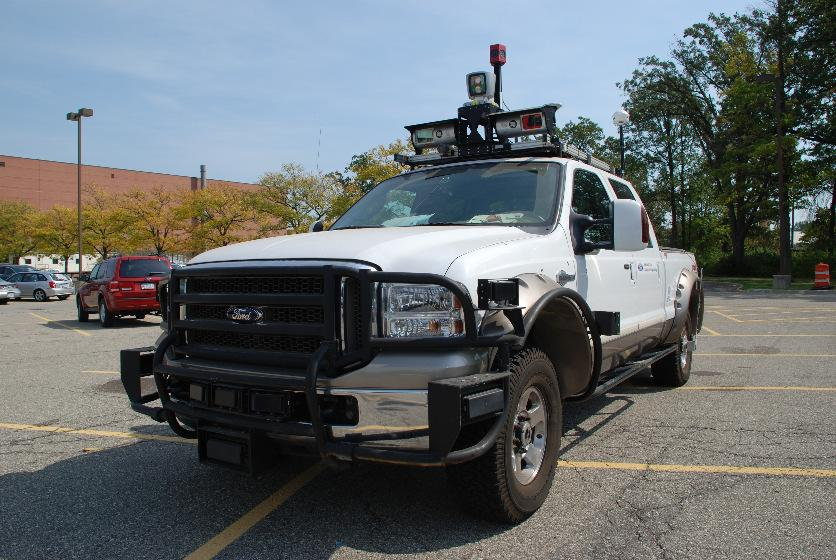
\includegraphics[width=0.5\textwidth]{img/sensor_fusion/ford_sensors.jpg}
	\caption[Ford 250 used to acquire Ford Campus dataset.]{Ford 250 pickup equipped with some sensors described in the Section~\ref{sec:introduction:scope_motivation}. On the top, the Ladybug omnidirectional camera, on the back the \ac{imu} and \ac{gps} unit.}
	\label{fig:sota:ford_sensors}
\end{figure}

The data is provided in raw format, accompanied by log files with timestamps, \ac{gps} and \ac{lcm}\footnote{For more information on \acf{lcm} protocol for estimating delays between sensory data registration on master-slave systems, see~\cite{Huang2010a}.} logs with all raw data. The images from an omnidirectional camera %, a Point Grey Ladybug3, 
are stored on \ac{ppm} and \ac{lidar} data %from a Velodyne HDL-64E
on \ac{pcap} format, from the \ac{tcp} connection socket.%; two Riegl LMS-Q120 \acp{lidar} also provide more information on the scan.

Rectified and synced data is stored in \ac{matlab} \textit{.mat} files. Along with the raw data and synced and rectified \textit{.mat} files, source code is also provided for parsing the raw data, visualizing the \ac{lcm} logs and pre-processed data on \ac{matlab}. Software that can render textured point clouds, implemented in C and \ac{opengl}, is also provided.


\subsection{\acl{kitti} Dataset}
A well known dataset for researchers of computer vision, autonomous driving and \ac{ml}, \ac{kitti} was recorded in 2011 and released to the public in 2013. This dataset contains various driving scenarios: suburban, highways, residential and campus areas; with trucks, cars, cyclists and persons. Alongside with data for testing, calibration measures are provided for all sensors.

The test car, a Volkswagen Passat, is equipped with two stereo pairs, one with color and one with gray cameras, a \ac{lidar}, an \ac{imu} and a \ac{gps} sensor, is shown in Figure~\ref{fig:sota:kitti_sensors}. Data from all four cameras is stored on \ac{png} format, \ac{lidar} measurements stored as a binary float matrix, and \ac{gps} and \ac{imu} are saved textually. Additionally, the raw data logs containing the timestamps and the transformations between the sensors are also provided. Labeled data is also available for some test scenarios in \ac{xml} files.

\begin{figure}[!ht]
	\centering
	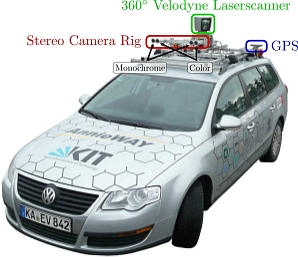
\includegraphics[width=0.5\textwidth]{img/sensor_fusion/passat_sensors.jpg}
	\caption[Volkswagen Passat used for recording \acs{kitti} dataset.]{Volkswagen Passat equipped with the sensors described in Section~\ref{sec:introduction:scope_motivation} graphs, for the \ac{kitti} dataset. On the top, the Velodyne \ac{lidar} and below the 2 stereo pairs (color and grey). On the back, the \ac{imu} and \ac{gps} systems are present.}
	\label{fig:sota:kitti_sensors}
\end{figure}


Along with the data and calibration parameters, several tools written in C++ or \ac{matlab} are also provided. The dataset offers two types of data categories: (1) unsynced and unrectified data or (2) synced and rectified data. The latter type is the one relevant for sensory calibration purposes.

The sensory apparatus contains 2 PointGray Flea2 greyscale and color cameras, a Velodyne HDL-64E \ac{lidar}~\cite{VelodyneHDL64}, among others less relevant sensors~\cite{Geiger2013a}.

\subsection{Udacity Self-Driving Car Nanodegree Dataset}
The data from Udacity online course on self-driving car is also publicly available~\cite{udacity}. This dataset dates to 2016 and was gathered to develop level 4 autonomy vehicles, containing much more data diversity than the previous two. The data available contains images from 3 color cameras,  \ac{lidar}, \ac{imu} and \ac{gps}, among other sensory data, such as speed, braking, etc.

This information is not available in raw format, only structured in \ac{ros} \textit{.bag} files. Some tools for visualizing and interacting with their data are provided for \ac{ros}~\cite{udacity}. 

Not much information about the sensors and their positioning is publicly available, and the dataset does not contain information for calibration.

\subsection{Summary}
Table~\ref{tab:sota:datasets_comparison} summarizes all the relevant data from the datasets~\cite{udacity, Pandey2011, Geiger2013a}. While there are few differences between the relevant types of data gathered, major differences can be observed on the format in which they are provided. 

The diversity of scenarios and size of the dataset is also an important aspect to consider. On this matter, \ac{kitti} and Udacity's are superior to Ford dataset, with \ac{kitti} providing the largest dataset in quantity, with already rectified and synced data. 
	
\begin{table}[!ht]
	 %\rowcolors{4}{gray!10}{white}
	 \renewcommand{\arraystretch}{1.2}
	 \centering
	 \begin{tabular}{@{}llccc@{}}
		 \toprule
		 \multicolumn{2}{l}{\multirow{2}{*}{Characteristics}} & \multicolumn{3}{c}{Datasets} \\ \cline{3-5}
																& & Ford Campus  & \acs{kitti} & Udacity \\ \midrule
																%
		 \multicolumn{2}{l}{\textit{Sensors and Data}} \\   \rowcolor{white}
		 \phantom{a}								& \ac{lidar}	   & \checkmark  & \checkmark & \checkmark \\ \rowcolor{gray!10}
																& Color Camera	 & \checkmark  & \checkmark & \checkmark  \\ \rowcolor{white}
																& Grey Cameras   &             & \checkmark &  \\ \rowcolor{gray!10}
																& Stereo Camera  &             & \checkmark & \checkmark  \\ \rowcolor{white}
																& Omnidirectional Camera &  \checkmark  &  &  \\ \rowcolor{gray!10}
																& \acs{imu}      & \checkmark  & \checkmark & \checkmark  \\ \rowcolor{white}
																& \acs{gps}      & \checkmark  & \checkmark & \checkmark  \\ \rowcolor{gray!10}
																& Driving data\footnotemark & & & \checkmark \\ \midrule \rowcolor{white}
		 \multicolumn{2}{l}{\textit{Data Formats and Tools}}  \\
		 \phantom{a}											 & Raw data available & \checkmark & \checkmark &  \\ \rowcolor{gray!10}
																			 & Data parsing tools & \checkmark & \checkmark & \checkmark  \\ \rowcolor{white}
																			 & Rectified data & \checkmark & \checkmark & \checkmark \\ \rowcolor{gray!10}
																			 & Synced data & \checkmark & \checkmark &  \checkmark  \\  \rowcolor{white}
																			 & Calibration parameters & \checkmark  & \checkmark  & \\ 
	   \bottomrule
		 \multicolumn{2}{l}{Raw data for sensors calibration} & \checkmark & \checkmark & \\ \rowcolor{gray!10}
		\multicolumn{2}{l}{\ac{ros} data compatibility} &  & \checkmark\footnotemark & \checkmark \\
		\multicolumn{2}{l}{Date of acquisition} & 2009  & 2011 & 2016 \\
		\bottomrule
	\end{tabular}
	\caption[Comparative analysis between the datasets.]{Comparison between the datasets more appropriated to this thesis objectives.}
\label{tab:sota:datasets_comparison}
\end{table}
\addtocounter{footnote}{-1}
\footnotetext{Other driving data includes, but it is not limited to: vehicle speed, joints states, twist, brakes, suspension, fuel level, \ac{can} bus data, steering, tire pressure, among many others.}
\addtocounter{footnote}{1}
\footnotetext{While Udacity dataset is the newest and provides direct out-off-the-shelf integration with \ac{ros}, that type of integration can also be achieved for \ac{kitti} by using other tools, such as \textit{kitti2bag}~\cite{TomasKrejci}.}

Comparing the 3 datasets using the information in Table~\ref{tab:sota:datasets_comparison} and the previous sections, Udacity and \ac{kitti} are better suited to the purposes of this work. They provide a larger dataset than Ford, have \ac{ros} compatibility and the tools provided are open-source and not developed to be used on proprietary software.

Since Udacity dataset integrates more easily with \ac{ros} than \ac{kitti}, providing also some tools for \ac{ros} preliminary tests, learning and earlier development stages were based on this dataset. Later, due to the lack of calibration parameters and raw data for sensors calibration\footnote{Note that, despite the Udacity dataset not providing data to ease the calibration of its sensors, such as camera intrinsic calibration or the extrinsic calibration between \ac{lidar} and camera, such calibration parameters can be obtained from this data. Those parameters are not as accurate as those obtained using a proper calibration setup and are out the scope of this work (being another research topic on itself) and therefore no effort will be dedicated to this topic.}, \ac{kitti} dataset was used instead.


%%%%%%%%%%%%%%%%%%%%%%%%%%%%%%%%%%%%%%%%%% CAMERA %%%%%%%%%%%%%%%%%%%%%%%%%%%%%%%%%%%%%%%%%%

\section{Camera as a sensor on \acl{cv} applications}
\label{sec:sota:camera}
Vision is the human sense most relevant to how we perceive the world and how we navigate in it~\cite{Ekstrom2015, Beck1983}. Replicating this ability on machines, through the usage of cameras, is a widely researched topic on computer vision and instrumentation~\cite{Beck1983}. The most common cameras, as our eyes, take advantage of the pinhole effect: a small hole (or pin), that is used to spatially filter the non-focused light beams through an aperture or lens~\cite{Beck1983, camera_models, Sturm2010}, producing a mirrored, but focused image.

On the following sub sections, basic notions of the current status of camera models and camera calibration are given. Since this research is focused strictly to the application of a camera as a sensor on computer vision, the overview provided abstains from describing extensive research on camera technologies and camera models for the field of computer vision. From a purely working principle and technologies, several camera types can be named, such as catadioptric, plenoptic, biprism, among others~\cite{Sturm2010}. %Considering consumer market, denominations such as Compact Cameras, \ac{dslr} cameras, Mirrorless (or \ac{evil} cameras) can also be used~\cite{comercial_cameras}. 
For further research, the reader might be interested on~\cite{comercial_cameras, Sturm2010, camera_models, Merklinger1993, Photopillers}.


\subsection{Camera Geometry}
\label{subsec:sota:camera-geometry}
A world point in a 3-dimensional Euclidean space can be represented by a vector with 3 real coordinates: $(X, Y, Z)$ and an image pixel of a digital image is typically represented as an element of a 2D matrix with integer coordinates $(u, v)$~\cite{mvg_book}. From a mathematical standpoint, a camera can be considered as a mapping tool between the world objects in three dimensions into a 2D image plan, such as depicted by Equation~\eqref{eq:camera_transform}, which leads to different mathematical models used to describe the camera~\cite{mvg_book, Sturm2010}.

\begin{equation}
	\label{eq:camera_transform}
	(X, Y, Z) \xrightarrow[]{\text{transformation}} (u, v)
\end{equation}

When describing camera models, several considerations should be made~\cite{Sturm2010}:
\begin{itemize}
	\item \textbf{Central Camera Models vs Non-Central Camera Models}: quantifies the number of optical centers on a camera. A central camera has only one optical center through which all light rays pass through to reach the film and a non-central has two or more optical centers;
	\item \textbf{Global vs Local models:} indicates if the parameters of the model are the same for all the image/\ac{fov} of the camera or if different regions of the image have different parameters, respectively.
\end{itemize}

For the application currently envisioned, global central camera models are considered. For a more detailed explanation of the topics above or an extensive overview of non-classical camera models, different types of projections and other aspects of modelling cameras, see~\cite{Sturm2010, camera_models}.

\subsubsection{Pinhole Camera Model}
Based on the pinhole effect, represented in Figure~\ref{fig:pinhole_effect}, the pinhole camera model is the most common camera model~\cite{camera_models}. The pinhole effect consists on using a small hole (or aperture) to spatially filter the light rays by angle of incidence, reducing the amount of light rays overlapping when coming from different incident angles through the pinhole, which otherwise would ``blur'' the image. 

\begin{figure}[!ht]
	\centering
	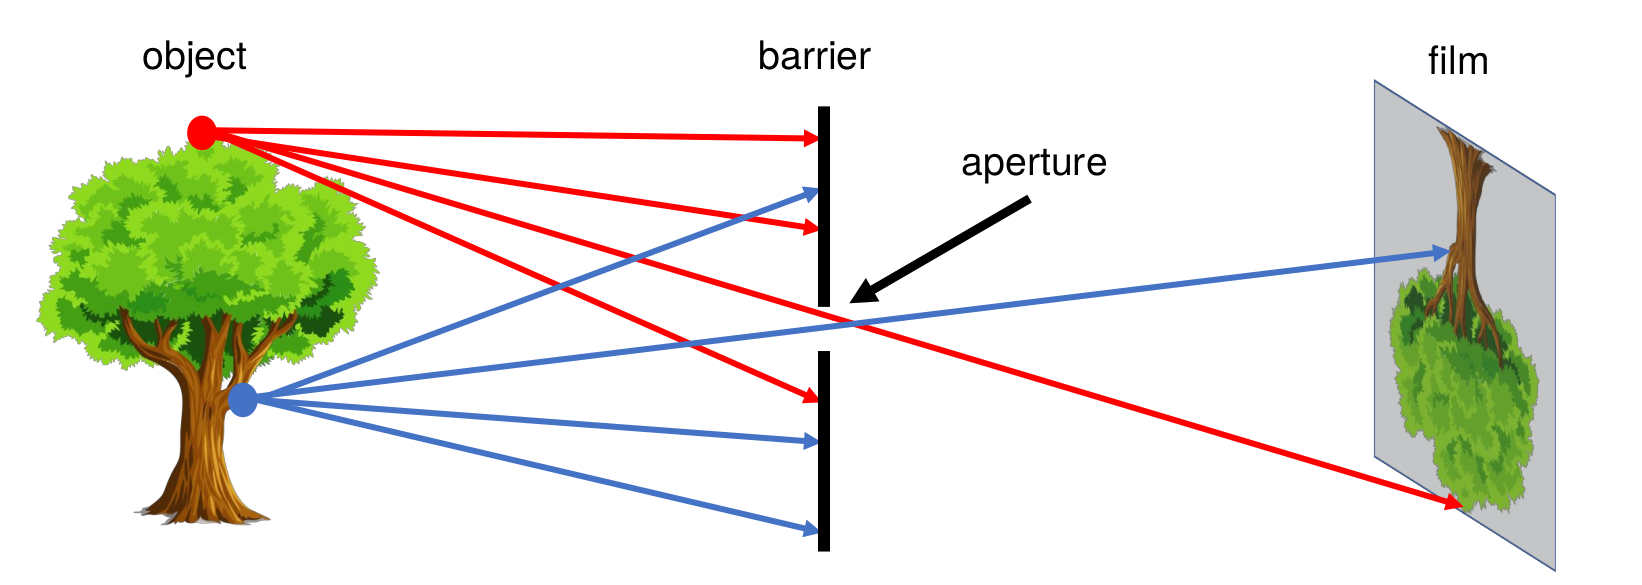
\includegraphics[width=0.6\textwidth]{img/camera/pnhole_effect.png}
	\caption[Pinhole effect on a small aperture.]{Pinhole effect on a small aperture. Source:~\cite{camera_models}.}
	\label{fig:pinhole_effect}
\end{figure}

The pinhole camera model describes the perspective transformation on Equation~\eqref{eq:camera_transform} as a central projection where all light rays meet at the camera center, $\mathcal{F}_c$. A diagram of the pinhole camera is shown in Figure~\ref{fig:pinhole_camera_model}. 

On this model, the z-axis is collinear with the optical axis\footnote{Also called principal axis. The two terms can be interchanged with no loss of context.}, aligned with the direction the camera is facing. The image plane is at $z = f$, where $f$ is the focal length, being intersected by the optical axis on the principal point, with coordinates $(c_x, c_y)$ on the image plane axis. Note that the principal point is not the origin of the referential on the image plane, but instead the middle point, being the origin located in the top left corner, with a downward y-axis.

\begin{figure}[!ht]
	\centering
	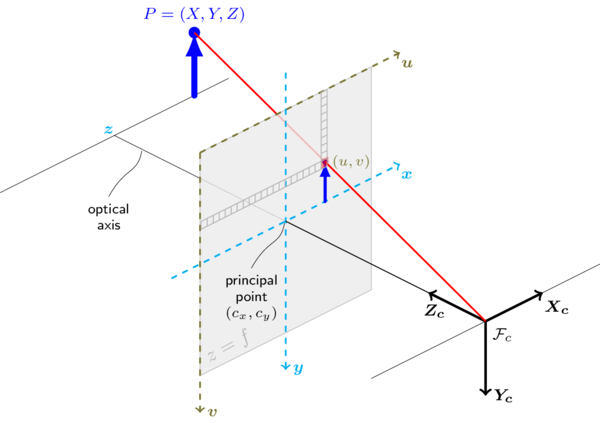
\includegraphics[width=0.6\textwidth]{img/camera/pinhole_camera_model.png}
	\caption[Pinhole camera model.]{Pinhole camera model. Source:~\cite{opencv_doc}}
	\label{fig:pinhole_camera_model}
\end{figure}

Due to the nature of the pinhole camera model, it is more convenient to use a Projective Space instead of the more common Euclidean Space~\cite{mvg_book, camera_models, Sturm2010}. On a Projective Space, as in a central camera model, all of its points are oriented through a single point~\cite{mvg_book}. Therefore, by using a projective space instead of a Euclidean for addressing the transformations of a pinhole camera model, becomes more intuitive and relatable to the actual geometry of the model. Despite projective spaces using homogeneous coordinates and non-Euclidean geometry, homogeneous coordinates can be converted for cartesian coordinates without loss, if the homogeneous points are possible to represent on a Euclidean coordinate frame~\cite{mvg_book, camera_models}.

\subsubsection{Projective Geometry}
A tridimensional Euclidean Space can be represented on a Projective Space using 4 coefficients. Therefore, the previous tridimensional vector can be rewritten in homogeneous coordinates as $(wX, wY, wZ, w)$~\cite{mvg_book}. If $w \neq 0$, we can transform from the Projective to Euclidean Space, obtaining the world representation of such points by dividing the homogeneous point by $w$. For the cases in which $w =  0$, we have purely projective points at infinity, that only exist in Projective Space~\cite{mvg_book}. 

The relation depicted in Equation~\eqref{eq:camera_transform} can be expressed in projective geometry as in Equation~\ref{eq:projective-geometry-pixel}, where $P$ represents the projection matrix that performs the transform from world points to image pixels. 

\begin{equation}
	\label{eq:projective-geometry-pixel}
	\begin{bmatrix}
		u \\ v \\ 1
	\end{bmatrix}
= P \times 
\begin{bmatrix}
		X \\ Y \\ Z \\ 1
\end{bmatrix}, \qquad \text{if } w = 1.
\end{equation}

The projection matrix in a pinhole camera model is the result of multiplication of two matrices: the camera matrix (or matrix of the camera's intrinsic parameters), $K$; and a joint rotation and translation matrix, $[R|t]$, where $R$ is the rotation matrix and $t$ the translation vector. The combination of these matrices is given on Equation~\eqref{eq:projective_matrix} and the full camera transform is expanded on Equation~\eqref{eq:camera_transform_full}, through the replacement of Equation~\eqref{eq:projective_matrix} in Equation~\eqref{eq:camera_transform}.

\begin{equation}
	\label{eq:projective_matrix}
	P = K[R|t]
\end{equation}

\begin{equation}
	\label{eq:camera_transform_full}
	\begin{bmatrix}
		u \\
		v \\
		1
	\end{bmatrix}
	= 
	\overbrace{
		\underbrace{
			\begin{bmatrix}
				f_x & 0 & c_x \\
				0 & f_y & c_y \\
				0 & 0 & 1 
			\end{bmatrix}
		}_\text{\large\textbf{K}}
		\underbrace{
			\left[
				\begin{array}{ccc|c}
					r_{xx} & r_{yx} & r_{zx} & t_x \\
					r_{xy} & r_{yy} & r_{zy} & t_y \\
					r_{xz} & r_{yz} & r_{zz} & t_z 
				\end{array}
		\right]
		}_\text{\large\textbf{[R|t]}}
	}^\text{\large\textbf{P}}
	\begin{bmatrix}
		X \\
		Y \\
		Z \\
		1
	\end{bmatrix}
\end{equation}

The matrix of intrinsic parameters is used to represent the calibration parameters of the camera: the focal lengths of each axis, $f_x$ and $f_y$, which scale the $x$ and $y$ axis; the principal point offset to the axis origin, $c_x$ and $c_y$, for the x and y-axis, respectively, that translate the image center with relation to the origin of the camera referential. 

The joint rotational-translation matrix, $[R|t]$, is also known as the extrinsic camera parameters, translates the coordinates of a point to the Cartesian coordinate system fixed to the camera.


\subsubsection{Cameras, Lenses and Distortion}
Using a simple pinhole for filtering light rays 
%, that would blur the image severely, 
reduces the amount of light reaching the camera sensor. Therefore, a lens is used to collect the light and focus it onto the image plane, providing the same effects as the hole~\cite{Sturm2010}, while allowing more light to be captured. The paraxial refraction model is represented in Figure~\ref{fig:pinhole_with_lense}, from which we can consider the Pinhole Camera model by letting $z_0 = 0$, which implies $z' = f$ and the image is formed on the focal point.

%pinhole effect with a lens is depicted 

\begin{figure}[!ht]
	\centering
	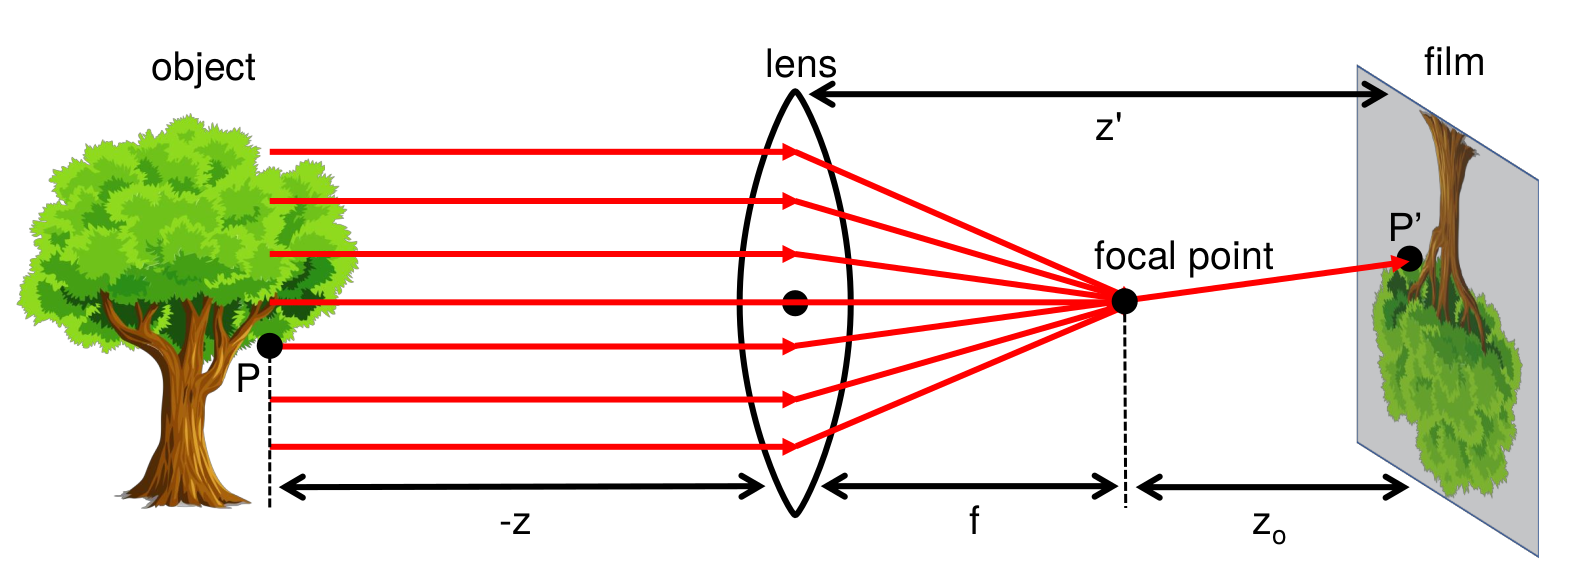
\includegraphics[width=0.6\textwidth]{img/camera/pinhole_with_lense.png}
	\caption[Pinhole effect on a lens]{Pinhole effect on a lens. Source:~\cite{camera_models}}
	\label{fig:pinhole_with_lense}
\end{figure}

Since lenses introduce non-linear distortion, the pinhole camera model needs to be extended to included radial and tangential distortion parameters~\cite{Bouguet2010, manuapphotogrammetry, Heikkila1997}. Such parameters indicate how the non-linear distortion of the camera lenses affects the image projection on the camera plane~\cite{camera_models, Sturm2010} and how can this be corrected~\cite{Heikkila1997, Bouguet2010, opencv_doc}. The equations behind that expression are beyond the scope of this introduction and therefore will not be detailed here, but the effect of lens aberration can be seen in Figure~\ref{fig:lense_distortion_types}.

\begin{figure}[!ht]
	\begin{subfigure}[c]{0.3\textwidth}
		\centering
		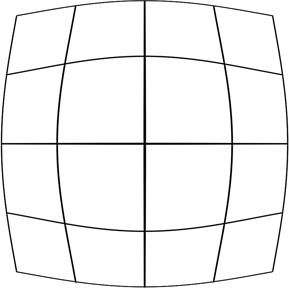
\includegraphics[width=0.6\textwidth]{img/camera/distortion-barrel.png}
		\caption{}
		\label{fig:barrel-distortion}
	\end{subfigure}
	%\quad 
	\begin{subfigure}[c]{0.3\textwidth}
		\centering
		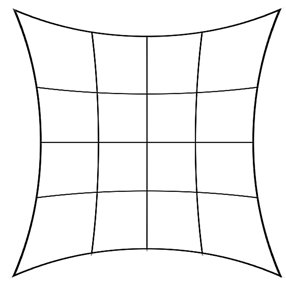
\includegraphics[width=0.6\textwidth]{img/camera/distortion-pincushion.png}
		\caption{}
		\label{fig:pincushion-distortion}
	\end{subfigure}
	%\quad
	\centering
	\begin{subfigure}[c]{0.3\textwidth}
		\centering
		
\includegraphics[width=0.6\textwidth]{img/camera/no-distortion.png}
		\caption{}
		\label{fig:no-distortion-lens}
	\end{subfigure}

	\caption[Effects of barrel and pincushion distortion caused by a non-linear klens.]{Barrel~(\subref{fig:barrel-distortion}) and Pincushion~(\subref{fig:pincushion-distortion}) distortion caused by the non-linear behavior of the camera lens. The effect of an ideal lens, with no distortion, is shown on~(\subref{fig:no-distortion-lens}). Source:~\cite{camera_models}.}
	\label{fig:lense_distortion_types}
\end{figure}

For more information on the pinhole camera model and lens distortion, see Hartley and Zisserman Multi View Geometry in Computer Vision~\cite{mvg_book}, Hata and Savarese course notes~\cite{camera_models} or \acf{opencv} official documentation~\cite{opencv_doc}. 

\subsection{Camera Intrinsic Calibration}
\label{subsec:sota:camera-intrinisc-calibration}
Calibrating a camera is the process in which the parameters of the model that describes its behavior are determined. For the extended pinhole camera model, this means determining the parameters of its intrinsic matrix, $K$, but also the distortion coefficients of the lens used~\cite{mvg_book, camera_models, Bouguet2010, Heikkila1997}. These parameters are called the intrinsic parameters and are independent of the scenario being viewed, if the focal length is kept constant. On the other hand, extrinsic camera parameters are different for every situation and therefore scenario dependent~\cite{opencv_doc, Bouguet2010, Heikkila1997}.

Zhang proposed in 2000 a method for calibrating a camera that unlike previous work, does not require a special setup, expensive experimental apparatus or complicated calibration patterns: it uses a planar object with a known pattern, which can be freely moved in front of the camera~\cite{Zhang2000}. Only two images are necessary for camera calibration, as long as the pattern movement between them is not a pure translation. The estimation of the camera intrinsic parameters and distortion caused by the lenses can be determined by solving Equation~\eqref{eq:camera_transform_full}, once several $2D \leftrightarrow 3D$ correspondences have been established.

Zhang's algorithm differs from other algorithms at the time that attempted to calibrate a camera by rotating it on a static environment. Other alternatives include Tsai's algorithm~\cite{Roger1987, mvg_book}, a 2-stage technique for camera calibration first presented in 1987, that does not determine the camera center. A \ac{dlt} algorithm can also be used to determine the camera calibration parameters (see~\cite{mvg_book}).

Following Zhang's algorithm, the correspondences between the 2D and 3D representations of the pattern can be made by finding the corners or circles on planar patterns~\cite{opencv, mvg_book}. Chessboards are the most common patterns used today~\cite{opencv}, allowing corner detection for each cell (Figure~\ref{fig:opencv_calib_pattern}). Since the dimensions of the cell and their arrangement are known previously, it is possible to compute the orientation of the chessboard~\cite{Zhang2000, opencv_doc, mvg_book}. On those conditions, revisiting Equation~\eqref{eq:camera_transform_full}, only the $K$ matrix is left to be determined. 

\begin{figure}[!ht]
	\centering
	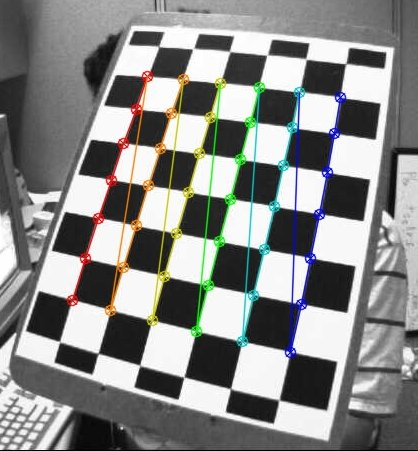
\includegraphics[width=0.4\textwidth, keepaspectratio]{img/camera/calib_pattern.jpg}
	\caption[Chessboard calibration pattern with the corners used for calibration.]{Chessboard calibration pattern with the detected corners overlapped. Source:~\cite{OpenCV_camera_calib}.}
	\label{fig:opencv_calib_pattern}
\end{figure}

The intrinsic calibration matrix coefficients can then be refined using a maximum-likelihood estimation to minimize the error using a non-linear method, such as Levenberg-Marquardt optimization~\cite{Levenberg1943}. Other optimizations are possible, such as Powell’ dog-leg non-linear least squares technique~\cite{Lourakis2005}. Further reading can be conducted on~\cite{mvg_book, Sturm2010, camera_models, Hata, Xu1996a}.

Bouguet in 2010 provided a Camera Calibration toolbox for \ac{matlab}~\cite{Bouguet2010}, which serves as the basis for many camera calibration toolboxes nowadays, such as \ac{opencv}, which is also based on the work of Zhang~\cite{opencv}.

\subsection{Image Processing Libraries for \acl{cv}}
In the field of computer vision, several tools and libraries are available, capable of performing low image operations, image detection, filtering, among others. This sub-section will list and briefly describe these tools.

\begin{itemize}
	\item \textbf{BoofCV~\cite{boofcv}:} written in Java, this library is oriented to real-time image operations, such as low-level image processing, camera calibration and feature/object  detection, tracking and recognition;
	\item \textbf{Dlib~\cite{dlib}:} modern C++ toolkit containing \acl{ml} algorithms and tools, some on the field of computer vision;
	\item \textbf{\ac{matlab} Computer Vision Toolbox\texttrademark~\cite{matlabcvtoolbox}:} toolbox for computer vision algorithms, 3D vision, and video processing systems. Can perform object detection and tracking. Detects, extracts and matches features;
	\item \textbf{\acf{opencv}~\cite{opencv}:} open source library for C++, Python and C that implements the state of the art algorithms on computer vision;
	\item \textbf{Vlfeat~\cite{vlfeat}:} open source library for C that implements many state of the art algorithms on computer vision;
	\item \textbf{SimpleCV~\cite{simplecv}:} Open source framework, written in Python, that can be used to implement computer vision software using other libraries;
\end{itemize}

Since a goal of this work is to use Open-Source tools as far as possible (instead of using closed source tools or code that is harder to integrate with other libraries), which is common among the automotive industry on the field of autonomous vehicles, \ac{matlab} \acl{cv} Toolbox\texttrademark~does not suit. The code of this work is mainly developed in C++, so Python and Java libraries will not be considered, resulting only in \ac{opencv} and Dlib, since Vlfeat uses plain C. 

\ac{opencv} has a large and active community and is considered by many researchers and industry leaders as the \textit{de facto standard} library regarding computer vision. Dlib is a robust library, but no significant differences can be seen when comparing with \ac{opencv}. Therefore, the final choice for a computer vision library is \ac{opencv}, also because of the already implemented compatibility with \ac{ros}.



%%%%%%%%%%%%%%%%%%%%%%%%%%%%%%%%%%%%%%%%%%% LIDAR %%%%%%%%%%%%%%%%%%%%%%%%%%%%%%%%%%%%%%%%%%

\section{Automotive \ac{lidar}}
\label{sec:sota:automotive-lidar}
\ac{lidar} sensors map their surroundings thanks to their high spatial resolution and capability of precisely measuring depth. Already used in topography, spectrography and air pollution studies, \ac{lidar} found its importance on the automotive industry as one of the key sensors of autonomous cars and \ac{adas}~\cite{Sullivan2016}. 

The maps produced by \ac{lidar}, commonly represented as point clouds or mesh clouds models (Figure~\ref{fig:bunny}), are one of the preferred method for \ac{slam} algorithms, which allow a vehicle without previous knowledge of its surroundings to autonomously navigate them, a crucial task for \ac{adas} on self-driving vehicles.

Point clouds represent the spatial data measured by the \ac{lidar} as points on the tridimensional space. The objects represented on a point cloud are formless, as they have no relation with their ``adjacent'' points, as depicted in sub-Figure~\ref{fig:bunnyPointCloud}. A Mesh cloud representation of the point cloud in sub-Figure~\ref{fig:bunnyMeshCloud}, produced from by the point cloud in sub-Figure~\ref{fig:bunnyPointCloud}, is a representation of the same points united by lines, forming a mesh. A mesh cloud conveys form, as can be verified by comparing the point cloud with the mesh representation of the same data. A mesh cloud, contrary to a point cloud, can also represent a close form and therefore having a volume.

\begin{figure}[!ht]
	\centering
	\begin{subfigure}[c]{0.45\textwidth}
	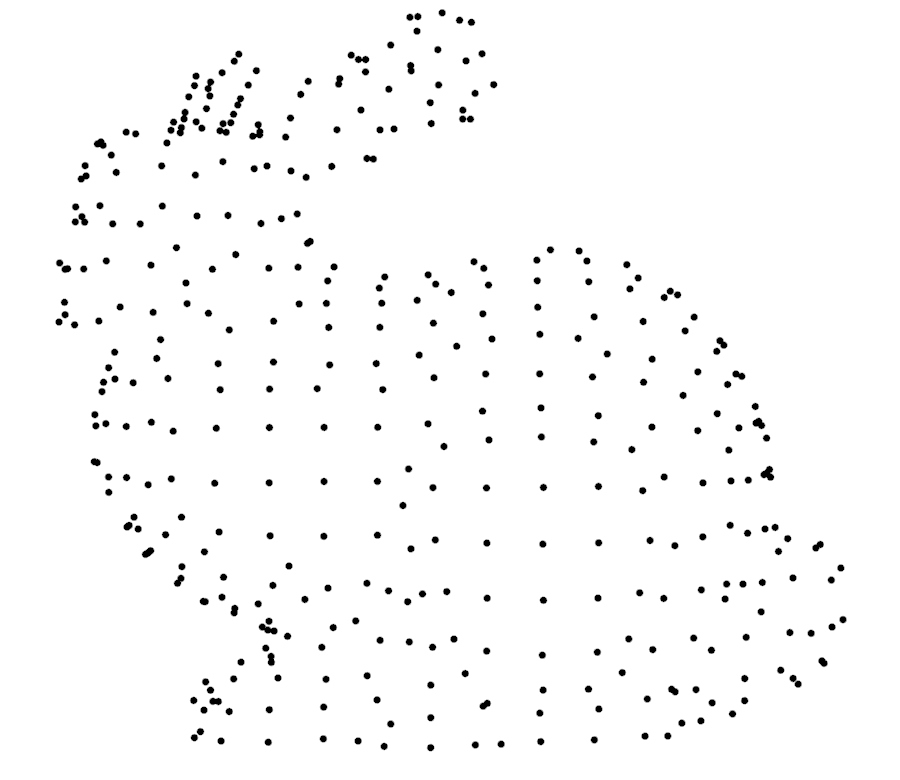
\includegraphics[width=\textwidth]{img/lidar/bunny_point.png}
		\caption{Point Cloud representation}
		\label{fig:bunnyPointCloud}
	\end{subfigure}
	\quad
	\begin{subfigure}[c]{0.4\textwidth}
		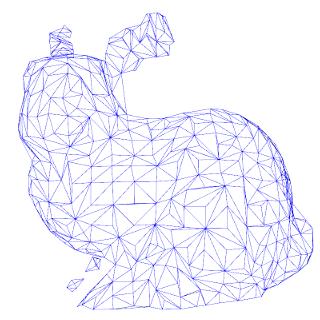
\includegraphics[width=\textwidth]{img/lidar/bunny_mesh.png}
		\caption{Mesh Cloud representation}
		\label{fig:bunnyMeshCloud}
	\end{subfigure}
	\caption[Example of a point and mesh clouds.]{Stanford bunny~\cite{bunny} point cloud (\subref{fig:bunnyPointCloud}) and mesh cloud (\subref{fig:bunnyMeshCloud})}
	\label{fig:bunny}
\end{figure}

\subsection{\ac{lidar} classification based on the depth measurement principle}
Regarding the type of signals and principles for measuring the scene distance, \acp{lidar} can be either \ac{cw} (emit a sinusoidal or square modulated signal), pulsed (emit a square pulse at fixed moments in time)~\cite{Payne2009, TexasLiDAR, SpringerOptics} or other more exotic and experimental types, that will not be addressed here, since they are out of the scope of this work.

\ac{cw} \acp{lidar} continuously emit a modulated \ac{laser} signal to their surroundings and, depending on the modulation technique, this signal can either be \ac{am} or \ac{fm}\cite{TexasLiDAR}. \ac{am}\ac{cw} \acp{lidar} operates by emitting a pseudo-random stream of binary data and coherently detecting the received signal. The phase shift distance, measured between the emitted and received signal, is directly related with the distance at which the pulse was reflected.

If \ac{fm}\ac{cw} is used instead, the \ac{lidar} \ac{laser} sends a frequency chirp\footnote{A signal whose frequency varies linearly with time.} and coherently detects the received signal, estimating the distance at which the reflection occurred (i.e., the distance at which the object is), by the frequency shift between the emitted and reflected signals~\cite{Payne2009, TexasLiDAR}. Coherent detection can be performed by heterodyne or homodyne detection, but such details will not be addressed here. A brief description and comparison between the two detection modes applied to \ac{lidar} technology is given in~\cite{Conroy2009}, and the underlying theory can be consulted on~\cite{Carlson2010, SpringerOptics}.

Pulsed \ac{lidar} technology acquires depth information by measuring the \acf{tof} between the reflection and emission of the same light pulse by the \ac{lidar} \ac{laser}. This technology is the most common type used for measuring depth on automotive \ac{lidar}~\cite{Sullivan2016}, and therefore this work will be based on pulsed~\ac{tof} technology to measure the distance at which the obstacles on the scene are present.

Both \ac{cw} and \ac{tof} \ac{lidar} have advantages and disadvantages, but they will not be compared here. Further reading about the topic can be found on~\cite{Sullivan2016, Simonite2017, Payne2009, TexasLiDAR}.


\subsection{\ac{lidar} classification based on construction}
Despite the depth measurement technique used by \ac{lidar} devices, regarding its construction and mapping technology, automotive \acp{lidar} can be one of the following categories~\cite{Hecht2018, Sullivan2016}:

\begin{enumerate}
	\item \textbf{Rotating \ac{lidar} or Macro-scanners:} the most common type, the \ac{lidar} optical and electrical circuit are mounted on a mechanical rotating device, which normally results on a wider \ac{fov} than the other models~\cite{Sullivan2016};
	\item \textbf{Flash:} organized in a matrix structure, similar to a standard \ac{ccd} or a \ac{cmos} camera, every element of the matrix contains a photodetector. A ``flash'' simultaneous illuminates all the \ac{fov}, and the reflected light intensity and time of arrival is measured to provide depth calculations, simultaneously for all pixels of the depth image~\cite{TetraVue, Ouster, Gelbart2002,Stettner2010, Simpson2019}; 
	\item \textbf{\ac{mems}:} operate by controlling the angle at which a rotating microscopic mirror is aligned with the \ac{laser}. By varying the angle, a single line can be scanned and using multiple \acp{laser} with the same mirror allows vertical scan~\cite{LeddarTech, Yoo2018};
	\item \textbf{Phased Arrays:} still on an embryonic stage, phased array \ac{lidar} use a microscopic array of antennas, similar to a \ac{radar}, where the phase of each antenna is individually controlled to allow the \ac{lidar} to sweep and/or focus on a specific area, using beamforming theory~\cite{Quanergy2018, Yu2016}.
\end{enumerate}

Of all the four types of \ac{lidar} presented, \ac{mems} and phased array \ac{lidar} are still unsuited for autonomous vehicles, since they have yet to leave their early research state and develop a functional prototype~\cite{Sullivan2016, Hecht2018}. 

Flash \acp{lidar}, also referred by some authors as solid state \ac{lidar}, since it has no movable parts, has the potential to become the most reliable, durable and cheaper \ac{lidar} technology~\cite{Sullivan2016, Hecht2018, Fersch2017a}. However, this technology is not yet mature, with some of its best experimental  prototypes achieving a maximum distance of \SI{2}{\meter}~\cite{Hecht2018}. The main cause for such lower range is the attenuation of the flash intensity, since its power is inversely proportional to the squared distance and the power the can endure.

Some prototypes are also unveiled from startups, such as TetraVue~\cite{TetraVue} and Ouster~\cite{Ouster}, and some patents are being registered~\cite{Simpson2019}; but this \ac{lidar} technology is not yet suited for the automotive market of autonomous cars~\cite{Fersch2017a}.

Therefore, only one alternative remains: a mechanical rotating \ac{lidar}, which is the technology that will be chosen for this work.

\subsection{The Mechanical Rotating \ac{lidar}}
To construct a rotating \ac{lidar}, a single pair of \acp{laser} and photodetectors are assembled on a fast rotational device (typically \SIrange{5}{20}{\revspersecond}), allowing that pair to scan a single line while rotating, creating a 2D \ac{lidar}. If multiple pairs are assembled with different polar angles, the \ac{lidar} is said to be a 3D \ac{lidar}, since a total revolution can produce a three-dimensional map of its surroundings~\cite{Sullivan2016}.

While a rotating \ac{lidar} consumes more power than the other counterparts, it can also achieve ranges until 100 meters~\cite{vlp16, Sullivan2016} or even 200 meters~\cite{VelodyneHDL64, Pandar40UserGuide, Sullivan2016}. To measure the depth on a rotational \ac{lidar}, \ac{tof} is the most common technique, being the pulse triggered at a defined angular step when rotating.

Regarding rotating \acp{lidar} technology, only 5 relevant companies exist worldwide. Velodyne\cp~\cite{Velodyne}, HESAI\cp~\cite{Hesai}, RoboSense\cp~\cite{Robosense}, Ouster\cp~\cite{Ouster} and Quanergy\cp~\cite{Quanergy}. Velodyne is the undisputed market leader~\cite{Sullivan2016, Hecht2018}, with several rotating \ac{lidar} solutions, ranging from \SIrange{16}{128}{} \ac{laser} beams.

Quanergy is a \ac{lidar} company that is focused on bringing solid state \ac{lidar} to the market. They provide one mechanical rotation \ac{lidar} solution, but with only 8 beams, which is not suited for the demands of autonomous driving~\cite{Sullivan2016, Hecht2018}. 

Ouster is a startup that produces mechanical rotational \acp{lidar}. They have two models, \texttt{OS-1} and \texttt{OS-2}, for mid and large range, respectively, which differ on their \ac{fov}, range and number of beams~\cite{Ouster}.

HESAI and RoboSense are two Chinese \ac{lidar} manufacturers whose products are similar to Velodyne's. In fact, they are so similar that a lawsuit as been filled against them by Velodyne, for intellectual property issues~\cite{VelodyneLawsuit}. This lawsuit is due to Velodyne holding the patent on mechanical rotating \acp{lidar} with surround view\cite{Hall2011}, which ensures its dominance on the market of mechanical \acp{lidar}. 

In fact, on their specifications, \acp{lidar} from Velodyne, HESAI, RoboSense or Ouster differences are \ac{laser} position managing, range and vertical \ac{fov}. On the other hand, they severely differ in terms of prices, with top of the range Velodyne \ac{lidar} selling for $\$85000$ and the cheaper at some thousand dollars. 

For our work, since Velodyne's is the top of the market solution and the more mature, it makes sense to test \ac{lidar} interference on the most used solution, since if two \acp{lidar} will interfere on the road, the most likely scenario is that they are from Velodyne's.

\subsection{Point Cloud Processing Software}
Considering only point cloud software targeted to developers and not final users, VeloView\texttrademark, a \ac{lidar} data visualizer by Velodyne is excluded as an alternative for this thesis, since it only allows to visualize data and save/load data from files. Similarly, programs that only intend to provide some features to apply to point clouds, and do not allow for research on point cloud processing to be conducted, are not viable solutions for this work. 

From the software that has not being excluded by the previous conditions, several point cloud processing libraries were researched and are detailed below:

\begin{itemize}
	\item \textbf{\ac{cgal}:}	a library containing geometric algorithms, written in C++, optimized for polygons and polyhedra processing, whose target are geographic information systems, such as computer aided design, molecular biology and robotics, among others~\cite{CGAL};
	\item \textbf{\ac{pdal}:} written in C++, \ac{pdal} is an adaptation of \ac{cgal} optimized to handle point cloud data. It is more oriented for the user to define a process pipeline in JavaScript, from already available algorithms on its library than for the developer to implement its own~\cite{PDAL};
	\item \textbf{Open3D:} written in C++, Open3D is a library optimized for common operation in point cloud processing, providing voxelization, nearest neighbor search, normal estimation and visualization interfaces, among other utilities~\cite{Open3D};
	\item \textbf{\acf{pcl}:} Open-Source and with an active community, \ac{pcl} is a large library for 2D/3D image processing and point cloud processing. It allows generic data types, has a comprehensive amount of state of the art algorithms and easily integrates with \ac{opencv} and \ac{ros}~\cite{PCL}.
\end{itemize}

All the alternatives are written in C++, the programming language of choice for this work. From the 4 libraries, \ac{cgal} is not optimized for point cloud data and \ac{pdal} intends to simplify routine point cloud processing, which is not aligned with the objectives of this thesis; for this reason, they are both excluded. Open3D and \ac{pcl} are reasonable alternatives, but \ac{pcl} modularity (allowing the user to define its data types) and extent of already implemented algorithms makes it a better solution than Open3D. Since we will also use \ac{opencv} and \ac{ros}, which \ac{pcl} allows integration with and this topic is widely detailed on forums, our choice for a point cloud processing library is \ac{pcl}.

\section{Camera and \ac{lidar} Extrinsic Calibration}
\label{sec:sota:extrinsic_calibration}

On a multiple sensor setup, coordinated frames from one sensor must be able to be referred on another sensor coordinate frame. Transforming data from one frame to another requires performing extrinsic calibration between them by determining the rigid body transform that can convert the data from one reference plan to the other without loss of information.

Therefore, the sole purpose of extrinsic calibration is to determine the coefficients of this transform, that can be described as a rotation and a translation, similarly to the joint rotation-translation matrix $[R|t]$ used for camera intrinsic calibration (Equation~\eqref{eq:camera_transform_full}). However, on this case, instead of this matrix representing the rotation of the object to the camera or the camera movement in the world, it represents the rotation and translation operations that need to be applied to the coordinate system of one sensor (and its data) to align the data with the coordinate system of another sensor. The precision of this transformation takes particular interest when data fusion (or sensor fusion) is being achieved, i.e., merging from this data sources to reduce errors and improve the significance of data each sensor is capable of giving. 

Several algorithms have been suggested for performing extrinsic calibration on data. They range from the necessity of well controlled environments to requiring no human intervention, using or not a calibration pattern. 


\subsection{Calibration using Patterns}
Typical extrinsic calibration between \ac{lidar} and camera with intersecting \ac{fov} use calibration patterns: Unnikrishnan first proposed a \ac{lidar} to Camera extrinsic calibration using a toolbox developed to manually select correspondences between a calibration pattern on image and point cloud~\cite{Unnikrishnan2005}. A \ac{matlab} toolbox to ease the process was also developed in 2005 by Unnikrishnan\etal~\cite{Unnikrishnan}. Fremont\etal uses a planar calibration target with a hole surrounded by a solid color, matching the depth discontinuities from the \ac{lidar} with the color discontinuities from the camera~\cite{Fremont2013} and Velas uses a planar pattern with geometric objects carved on its surface~\cite{MartinVelas2013}. Liao\etal proposes a method that only requires the usage of a planar polygon of known shape~\cite{Liao2019} and Park\etal tests and presents results of this calibration method applied to multiple polygons, specially with triangular shape~\cite{Park2014}. Mirzaei\etal uses a planar pattern with fiducial marker~\cite{Mirzaei2012}. 

Regarding calibration with three-dimensional calibration targets, Pusztai uses a box with different colors on each face~\cite{Pusztai2018}; Pereira uses a ball (for performing multiple sensor calibration, instead of only 3D \ac{lidar} and monocular camera)~\cite{Pereira2016}; Gong a trihedral object, determining the extrinsic calibration parameters using a nonlinear least squares algorithm~\cite{Gong2013}.

While the previous methods were focused on calibrating monocular cameras with tridimensional \ac{lidar}, alternative methods exist for stereo systems, taking advantage of the disparity map obtained with a stereo camera. Automatic methods are proposed by Geiger\etal and Guindel \etal. Geiger\footnote{One of the researchers behind \ac{kitti}.} and Moosmann propose a method for calibrating such setup with a single shot, using chessboards with multiple sizes and orientations. Their algorithm initializes seed point on the chessboard corners on image, and by region growing algorithms detects the chessboard position on camera, while on \ac{lidar}, planar detection and successive refinement is applied~\cite{Geiger2012a}. Guindel\etal use a planar calibration target with four holes that can be detected on the stereo map from the camera and \ac{lidar} point cloud, extrinsically calibrating both sensors by detecting the holes center and compute the rotation and translation that minimizes error. 

\subsection{Calibration without human intervention or patterns}
Some automatic methods that do not require human intervention neither calibration patterns have also been present on the literature. Bileschi's method estimates all intrinsic camera parameters  (including radial distortion) and the rotation and translation between a camera and \ac{lidar}, that is later refined by discontinuity association~\cite{Bileschi2009}. Naroditsky \etal proposes an automatic calibration method using the multi-polynomial Macaulay resultant, that, paired with \ac{ransac} and least-squares refinement, can automatically calibrate the camera-\ac{lidar} setup~\cite{Naroditsky2011}. Shaukat proposes a solution for planetary space robots based on  stereopsis and depth maps matching using mesh grids stecthing~\cite{Shaukat2016}. Ishikawa \etal calibration method, computes the calibration parameters using two main steps: first, it initializes the parameters from the movement of the camera and \ac{lidar} and secondly, refines those parameters using sensor-fusion until convergence~\cite{Ishikawa2018}. 

Jeong \etal presents a framework for calibrating \ac{lidar} and stereo cameras with non-overlapping \ac{fov}, by utilizing road markings and robust optimization algorithms and cost functions~\cite{Jeong2019}.

Using mutual information techniques, Taylor and Nieto's approach uses normalized mutual information between camera and \ac{lidar}, maximizing the features to be matched on a particle swarm map, with refinement techniques~\cite{Taylor2013}; Pandey's \etal approach defines a cost function for the mutual information and using known methods, minimize and refine the results to obtain the best parameters~\cite{Pandey2012}.


\subsection{Other calibration methods}
Other calibration techniques use data variation through time~\cite{Chien2017} or Deep learning on \ac{cnn}~\cite{Wang2018a}. Scaramuzza \etal introduce a simple technique for extrinsic calibration that does need calibration patterns~\cite{Scaramuzza}: instead it requires the user to manually select correspondences between the camera and \ac{lidar}, easing the selection with the transformation of point clouds to Bearing Angle images. Brabec offers advances on this method, using a semi-automatic process where correspondences between the camera and \ac{lidar} (presented as a directional image) data are selected by the user and refined using local correction and \ac{ransac} algorithms~\cite{brabec2014}.

Varuna De Silva \etal propose an approach based on the geometric positioning of the sensors on the setup, determining the parameters through geometric description between them, later refining this estimate using depth maps and a non-linear refinement technique (Gaussian Process Regression)~\cite{DeSilva2018}. In another of their works, a planar calibration pattern with holes is used, followed by the same refinement technique~\cite{Silva2018}.


\subsection{Summary of Extrinsic Calibration Techniques}
Multiple calibration techniques were described on this section, with some requiring special calibration patterns, others do not even require human intervention and some of them rely on deep learning and \ac{nn}. 

Extrinsically calibration between the \ac{lidar} and camera, if performed using a pattern,  requires the calibration object to contain relevant information to both the camera and the \ac{lidar}. A calibration pattern with relevance to the camera implies having a color or a known pattern. For the \ac{lidar}, depth discontinuities are required. In order to create a good calibration pattern with depth discontinuities, either it is bulky or the depth discontinuity is caused by a hole and therefore the distance to the background varies. Either way, such calibration method is not practical, therefore will not be used.

Relying on \ac{nn}, time variation or other exotic techniques will only add unnecessary complexity to this work, which would deviate us from the intended goals. Fully automatic methods would also require a large amount of time to implement, validate and tune to the experimental setup data, which is impractical.

From all the methods presented, our efforts will be placed on a semi-automatic solution, with refinement, that requires user interaction and then refines the calibration parameters estimated. Examples of such work are Taylor and Nieto's~\cite{Taylor2013}, Pandey's~\cite{Pandey2012},Scaramuzza~\cite{Scaramuzza}, Brabec~\cite{brabec2014} and Varuna~\cite{DeSilva2018}.


\section{Sensor Fusion}
\label{sec:sota:sensor-fusion}
Fusing sensory data is the task of combining different data formats, acquired by different sensors into a multi-modal view of the world. This multi-modal view not only allows a better interpretation of the individual data, but also allows the raise of higher context semantics, since fused data is more than the sum of its parts.

Sensor data needs to be preceded by proper extrinsic sensor calibration before data can be fused. For monocular RGB cameras and \ac{lidar}, sensor fusion translates to augmenting the depth information of a point cloud by adding color from the image obtained with the camera or overlapping on the camera image the distances at which objects appear on \ac{lidar} data. An example of a colored point cloud (retrieved from~\cite{Gong2013}) can be seen in Figure~\ref{fig:colored_point_cloud_example} and an image overlapped with \ac{lidar} distance measurements (retrieved from~\cite{Bileschi2009}) can be seen in Figure~\ref{fig:image_with_lidar_distance}.

\begin{figure}[!ht]
	\centering
	\begin{subfigure}[t]{0.55\textwidth}
		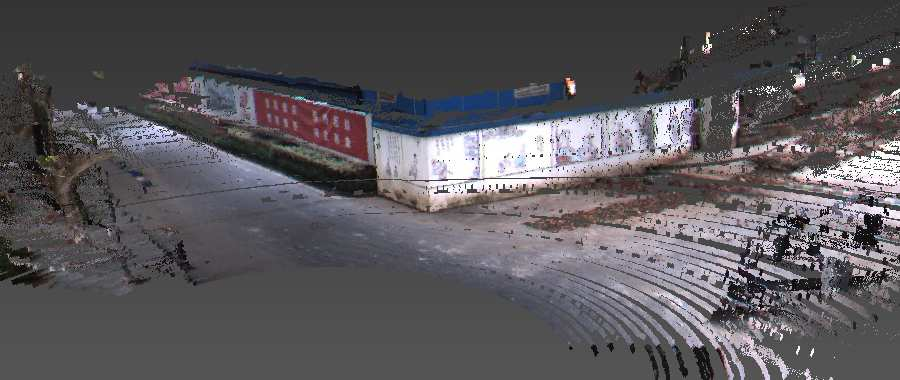
\includegraphics[width=\textwidth]{img/sensor_fusion/colored_point_cloud.png}
		\caption{Colored Point Cloud. Source~\cite{Gong2013}}
		\label{fig:colored_point_cloud_example}
	\end{subfigure}
	\quad
	\begin{subfigure}[t]{0.40\textwidth}
		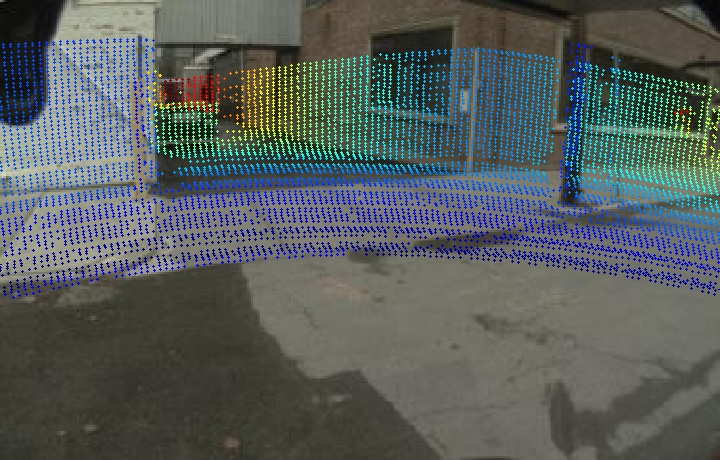
\includegraphics[width=\textwidth]{img/sensor_fusion/image_with_distance_point_cutted.png}
		\caption{Camera Image with overlapping distance measurements. Source~\cite{Bileschi2009}}
		\label{fig:image_with_lidar_distance}
	\end{subfigure}
	\caption[Examples of state of the art sensor fusion results between camera and \acs{lidar} data.]{Examples of sensor fusion between camera and \ac{lidar}. Sub-Figure~(\subref{fig:colored_point_cloud_example}) represents a colored point cloud, whose pixels are projected to the point cloud and nearby 3D points are colored with the color of their correspondent pixel. Since \ac{lidar} \ac{fov} is wider than the camera's, several points are black because no correspondences can be made. Sub-Figure~(\ref{fig:image_with_lidar_distance}) displays an image with overlapping distance measurements. Point cloud points in the image \ac{fov} are projected into the image and color mapped with intensity.}
	\label{fig:point_cloud_camera_fusion_example}
\end{figure}

There are three major types of sensor fusion: 

\begin{enumerate}
	\item \textbf{Calibration + Fusion:} Sensors are first calibrated among themselves, using one of the techniques described in Section~\ref{sec:sota:extrinsic_calibration}, and then data is converted to a referential of choice and merged;
	\item \textbf{Simultaneous Calibration and Fusion:} the implemented algorithms attempt to merge the data by minimizing an appropriated cost function. The final result consists on the multimodal merged data and the calculated extrinsic calibration parameters;
	\item \textbf{``Direct'' Sensor Fusion:} Genetic algorithms, neural networks or other similar tools analyze \ac{lidar} and camera data, without knowing any previous information about them, and output the merged data in the desired format.
\end{enumerate} 


\subsection{Calibration + Fusion}
\label{subsec:sota:calibration-and-fusion}
After calibrating the camera and \ac{lidar}, the data from these sensors can be fused, for a visual assessment of the correctness of the calibration. Some authors' whose work is referred on Section~\ref{sec:sota:extrinsic_calibration}, also show the results of sensory fusion applied to their data with the results of the proposed calibration algorithms, as a proof of calibration correctness. Unnikrishnan\etal~\cite{Unnikrishnan2005}, Velas\etal~\cite{MartinVelas2013}, Mirzaei\etal~\cite{Mirzaei2012}, Pusztai\etal~\cite{Pusztai2018} and Gong\etal~\cite{Gong2013} opt to use the camera information to color the point cloud, showing a colored point cloud (for Gong's\etal example, refer to sub-Figure~\ref{fig:colored_point_cloud_example}). Others, such as Fremont\etal~\cite{Fremont2013}, Liao\etal~\cite{Liao2019} and Park\etal~\cite{Park2014} prefer to show a visual metric of the calibration correctness by overlapping depth information gathered by the \ac{lidar} onto the image.

This sensor fusion technique is based on the application of the affine transformation described in Equation~\eqref{eq:jointRotationTranslationTransform}, which transforms data from the \ac{lidar} coordinate frame to the camera, allowing for a $3D point \leftrightarrow pixel$ mapping, enabling either point cloud coloring or overlapping the distance measurements on the image, as previously shown in Figure~\ref{fig:point_cloud_camera_fusion_example}.
	
\begin{equation}
	\label{eq:jointRotationTranslationTransform}
	\begin{bmatrix}
		X_{cam} \\
		Y_{cam} \\
		Z_{cam} \\
		1
	\end{bmatrix}
	= 
		\underbrace{
	\left[
			\begin{array}{ccc|c}
				r_{xx} & r_{yx} & r_{zx} & t_x \\
					r_{xy} & r_{yy} & r_{zy} & t_y \\
					r_{xz} & r_{yz} & r_{zz} & t_z \\
					0      & 0      & 0      & 1 
				\end{array}
		\right]
		}_\text{\large\textbf{[R|t]}}
	\begin{bmatrix}
		X_{LiDAR} \\
		Y_{LiDAR} \\
		Z_{LiDAR} \\
		1
	\end{bmatrix}
\end{equation}


\subsection{Simultaneous Calibration and Fusion}
\label{subsec:sota:simultaneous-calibration-fusion}
Li\etal proposes a method for simple indoor setups consisting of a single camera and a \ac{lidar} on a servo motor. The mechanism is rotated for three angular positions and a point cloud and image is taken for each one. Then, every image and point cloud are stitched together using fiducial features, resulting on a colored point cloud and on the determination of the calibration parameters~\cite{Li2016}. 

Park\etal also proposes a method for fusing uncalibrated \ac{lidar} and stereo camera data, using two \ac{cnn}: one for calibration, by reducing error between disparity images; and a second to refine the fused disparity maps with the left image~\cite{Park2019}. 

Yang\etal also proposes a method for stereo image and \ac{lidar} point cloud fusion using a Generalized \acl{icp} algorithm to match features and extracted a fused tridimensional refined model, at the same time it estimates the rigid body transform between camera and \ac{lidar}~\cite{Yang2017}.

Castorena\etal approach for sensor fusion matches the edges using a weighted total variation norm, fusing depth maps from a \ac{tof} camera with \ac{lidar} point clouds, useful not only for calibration, but also to refine the results of the fusion process and generate a more accurate colored point cloud~\cite{Castorena2016}.

\subsection{``Direct'' Sensor Fusion}
Still on embryonic steps, ``direct'' sensor fusion relies on deep learning to learn how to calibrate and fuse \ac{lidar} and camera data, therefore not requiring any previous knowledge about the dataset. It differs from sub-Section~\ref{subsec:sota:simultaneous-calibration-fusion} because the features and the cost function to be minimized are determined by the neural network and not projected by the researchers.

Liang\etal approach uses a multi-task multi-sensor dense fusion network for camera and \ac{lidar} fusion, that can not only fuse the data and create a colored point cloud, but also perform object detection on image and point cloud, with 3D bounding box estimation~\cite{Liang2019}.

Wei\etal research is aimed for a real-time multi-sensor collision avoidance system, on which the standalone usage of camera and \ac{lidar} does not yield satisfactory results~\cite{Wei2018}. The sensor fusion algorithm uses a \ac{cnn} and feature extraction to fuse \ac{lidar} and camera data. 

\subsection{Considerations about the different methods and our work}
On our work, since we are aiming to first calibrate the sensors and then fuse the data, following a more ``traditional'' approach to sensory data fusion, our algorithm will be based on the methods described in sub-Section~\ref{subsec:sota:calibration-and-fusion}. 

Simultaneous calibration and fusion methods (sub-Section~\ref{subsec:sota:simultaneous-calibration-fusion}) would be interesting, but the research focus to develop one of those methods would deviate our work from the \ac{lidar} interference study.

On the alternatives that rely on neural networks and deep learning, Wei\etal~\cite{Wei2018} solution is attractive, but it was only published when this work was in a final state, which made it not possible to be considered for this work.

\section{Object Detection}
\label{sec:sota:object-detection}

Object Detection is a field of \acl{cv} that intends to detect objects in an image. Currently, the most commons approach is a Deep-Learning based approach, where end-to-end object detection is possible without the need of handmade feature engineering.

%two approaches to tackle this problem are possible:

%\begin{enumerate}
%	\item \textbf{\acl{ml} based approach:} objection detection is performed on two steps: first a set of feature descriptors are chosen and extracted from reference images; secondly a \acf{nn} takes those features and perform the classification;
%	\item \textbf{Deep-Learning based approach:} end-to-end object detection without the need of handmade feature engineering.
%\end{enumerate}

%\subsection{\ac{ml} based approach}
%When referring to the first solution, Haar-like features~\cite{Messom2006}, \ac{sift}~\cite{Hughes2011a}, \ac{surf}~\cite{Bay2008} and \ac{hog} features~\cite{Dalal2010, Surasak2018} are normally used, on a Viola-Jones \ac{nn} (or its extensions)~\cite{Viola2001, ViolaP2004}. % For more details see 

\subsection{Deep-Learning based approach}
%The second solution is 
Normally implemented with a Region Proposal \acf{cnn}, developed by Girshick\etal on 2014~\cite{Girshick2014}. A common \ac{cnn} cannot be used for object detection on an image because the number of detected objects is variable, and so would be the size of the output layer, which is not possible on this architecture. A \ac{rcnn} differs from a \ac{cnn} due to the region proposal algorithm preceding it, that limits the number of regions to be evaluated on an image to approximately 2000, therefore limiting the number of objects on an image~\cite{Girshick2014}. However, this \acl{nn} needs to be run for every one of the 2 thousand regions, making it slow and infeasible for real-time object detection~\cite{Girshick2014}. One year later, Girshick proposed a new architecture called Fast \ac{rcnn}, that runs the convolutional model only once and generates a feature map and bounding box offsets, increasing the speed of its \ac{rcnn} up to 20 times and improving the \ac{map}~\cite{Girshick2015}, a common metric used to quantify the performance of \ac{nn} regarding their detection results. For further information and a formula, see~\cite{mAP, AP}.

In 2016, Shaoqing Ren\etal proposes a newer architecture that does not use a selective search for the region proposal algorithm, but instead has a Region Proposal Network to generate \ac{roi} for the proposal classification stage, called Faster \ac{rcnn}~\cite{Ren2017}. Such architecture achieves state-of-the-art object detection at a frame-rate of 5 \ac{fps}. 

Other alternatives, such as \ac{spp} Deep \ac{cnn}, exist and their details can be found in~\cite{He2015}.

While the previous \ac{nn} use separated networks for region proposal of a possible object on an image and region classification to locate a possible object on an image, \acf{yolo}, developed by Joseph Redmon, is an alternative solution that analyzes the image only once. It keeps a global context of the image while dividing it into regions and predicting bounding boxes. Those bounding boxes are weighted by the computed probabilities of each region and thresholding by the user~\cite{Redmon2016}. 

\subsection{Public Image Datasets}
To train deep learning image object detection \acp{nn}, several image datasets are available online. Two of the most relevant, considering number of labeled objects and number of images are:

\begin{itemize}
	\item \ac{pascal-voc} dataset;
	\item Microsoft \acf{coco} dataset.
\end{itemize}

\ac{coco}'s dataset has 80 object classes, containing common road objects also present on the \ac{kitti} dataset and other objects used on this research~\cite{Lin2014a}. Since \ac{pascal-voc} only has 20 object classes~\cite{Everingham2010}, being unable to detect a ball, truck and road signs, \ac{coco}'s dataset is preferred to train the image object detection \acp{cnn} weights.

\subsection{\ac{yolo}}
\ac{yolo}v2, released in 2017, can achieve, at best, 78.6 \ac{map} on the \ac{pascal-voc} 2007 dataset at 40 \ac{fps} (see more details in~\cite{Redmon2017}). \ac{yolo}v3, released in 2018, achieves, at best, 57.9 \ac{map}-50 on \ac{coco}'s dataset, at almost 20 \ac{fps} (3x faster than other networks with the same \ac{map}-50)~\cite{Redmon2018}.

\ac{yolo} runs on Darknet, an Open Source \ac{nn} framework written in C and \ac{cuda} by the same author~\cite{Redmon2013}. Darknet is configurable, supporting several network models without needed to be recompiled, such as AlexNet~\cite{Krizhevsky2007}, DenseNet~\cite{Huang2017}, ResNet~\cite{He2016}, \acp{rnn}~\cite{Cleeremans1989} and \ac{yolo}~\cite{Redmon2016}. It supports \ac{gpu} acceleration, if compiled together with Nvidia\cp~\ac{cuda}\texttrademark~library. Pre-trained weights for several image datasets and network models are available online on~\cite{Redmon2013}. 

\ac{yolo} is not the most accurate image object detection solution, but it is the only solution in the state of the art of image detection that offers a reasonable trade-off between accuracy, speed and resource usage~\cite{Redmon2018}. Therefore, it has proliferated as one of the most common \ac{nn} to be used on image detection, specially under scenarios where speed is important, such as autonomous vehicles. Therefore, \ac{yolo} is our preferred choice for an image object detection \ac{nn}.

\subsection{Cloud Based Platforms}
Several paid and cloud based alternatives exist, such as Amazon Rekognition~\cite{awsRekognition}, Google Cloud Vision \ac{api}~\cite{googlevision}, IBM Watson Visual Recognition~\cite{watson} and Microsoft Computer Vision software~\cite{azurecv}. 

Since those platforms require connectivity to the Internet, they are not good candidates to the solution we are trying to develop. Therefore, they are discarded.

\subsection{Objection Detection using \ac{lidar} and \ac{lidar} + Camera}
Out of the scope of this thesis is object detection only on \ac{lidar} data or \ac{lidar} + camera. However, as a starting point for object detection on point cloud, we recommend the work developed by Waleed Ali\etal~\cite{Ali2019}, which is an adaptation of \ac{yolo} to tridimensional data (point clouds): \ac{yolo}3D; and the work developed by Shi\etal~\cite{Shi2018}, a two part \ac{rcnn} that estimates and refines objects bounding boxes from point cloud data.

Regarding \ac{lidar} and camera simultaneous object detection, we recommend the familiarization with Complexer-\ac{yolo}, developed by Martin Simon\etal~\cite{Simon2019}, which is capable of detecting and tracking objects on point cloud and camera.


\section{\ac{lidar} Interference}
\label{sec:sota:lidar-interference}
\ac{tof} \ac{lidar}'s basic principle implies that when a \ac{laser} pulse is emitted, three different scenarios are possible, being the first one the only one that produces a valid measurement:

\begin{enumerate}
\item The \ac{laser} pulse returns, due to the reflection of an obstacle;
\item The \ac{laser} pulse does not return;
\item The \ac{laser} pulse returns with intensity below the noise floor.
\end{enumerate}

Interference and crosstalk between pairs of \acp{laser} and photodetectors on a \ac{lidar} are mitigated with different firing offsets, or in the case of mutual interference between \ac{lidar}, it is possible to synchronize their firing time using specialized clock signals~\cite{vlp16}.

However, in a society where self-driving vehicles coexist, another scenario is possible: \ac{lidar} ``A'' fires a \ac{laser} pulse that is received, directly or indirectly, by the photodetector on a \ac{lidar} ``B''. Since \ac{lidar} ``B'' measures the distance to an obstacle by measuring the time between the firing and reception of its own \ac{laser} pulse, the reception of another \ac{laser} pulse results in an erroneous measure with an unpredictable behavior. If this interference is significant, the reliability of the \ac{lidar}, and consequently autonomous vehicles and \ac{adas}, is seriously undermined due to the incapability to accurately map their surroundings.

% This problem, deeply researched for automotive \ac{radar} \cite{}, as yet to gain the attention of the research community of automotive \ac{lidar} and 


To the best of the author's knowledge, the first consideration about \ac{lidar} interference is given by Hebert and Krotkov in 1991~\cite{Hebert}. Their study was conducted for \ac{amcw} \ac{lidar} systems, and among other findings, they state that range and intensity measurements on \ac{lidar} are not completely independent, since lower intensity reflection can lead to an increase on range noise and shifts. 

In 2013, Retterath and Laumeyer~\cite{Retterath2015}, seek to provide an apparatus for an array based system with reduced interference. Their patented work is an array \ac{lidar} that has lower probability of crosstalk than other solutions, which was latter patented worldwide~\cite{Retterath2015WO}. In 2016, another patent is filled for the same array based \ac{lidar}~\cite{Retterath2016}, this time for object detection and in 2017, Facet Technology, the patent applicant, sends out a Press Release indicating that they have developed a \textit{``Safe and Secure\acs{lidar}\cp~Crosstalk Elimination Licensing Program''}, and that they have experienced crosstalk interferences up to 2\%~\cite{Facet}.

In 2017, Velodyne Inc., the world leader and  major manufacturer of mechanical rotating \ac{lidar}, filled a patent on a new implementation that reduces crosstalk~\cite{Hall2017}. Their focus is to solve inter-channel crosstalk, but multi-\ac{lidar} crosstalk reduction is also referred on the patent.

In 2018, Axel Diehm\etal proposes a spatial temporal filter for eliminating a crosstalk problem between two Velodyne HDL-64 \acp{lidar}~\cite{Hebel2018}. Their crosstalk behaviour is well-defined as an area of interfered points at a particular orientation, and their work is focused on how to filter out those points. They also partially expanded their analysis to the time domain of interference. Nonetheless, a root cause for the crosstalk behavior was not provided.

\subsection{Autonomous vehicles hacking through \ac{lidar} Interference}
Jonathan Petit\etal presents a study on how to remotely attack automotive cameras and \acp{lidar} on vehicles~\cite{Petit2015}. They explore several methods of attack, such as relay, replaying and spoofing. Petit's work shows, for laboratory scenarios, how to make obstacles disappear and how to make the \ac{lidar} see ``ghost'' objects, for distances further than the distance of the spoofer. 

Hocheol Shin\etal, two years later, presented an improved method that not only is able to spoof obstacles at a distance further than the distance of the spoofer, but also closer~\cite{Shin2017}. His work used common \acp{lidar}, such as Velodyne VLP-16~\cite{vlp16}. Shin\etal also found that the curved reception glass of \acp{lidar} allow for reflection of an attacking light source inside its case, allowing the attacker to be at a different direction that of the perceived attack. Despite their work being extremely experimental and not directly applied on real world scenarios, due to the laser alignment required for an effective attack on real driving scenarios, Petit\etal and Shin\etal research show that it is possible to attack a \ac{lidar} sensor and interfere with its measurements. Some results from Shin's research are shown in Figure~\ref{fig:shinInterference}.

\begin{figure}[!ht]
	\centering
	\begin{subfigure}[c]{0.4\textwidth}
	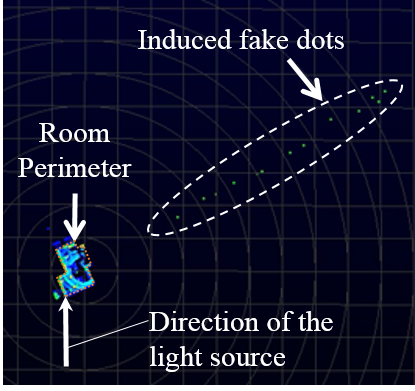
\includegraphics[width=\textwidth]{img/lidar/interference_angle_control.png}
\caption{}%Spoofing an obstacle at a different angle of the spoofer}
		\label{fig:shinInterferenceAngle}
	\end{subfigure}
	\quad
	\begin{subfigure}[c]{0.55\textwidth}
		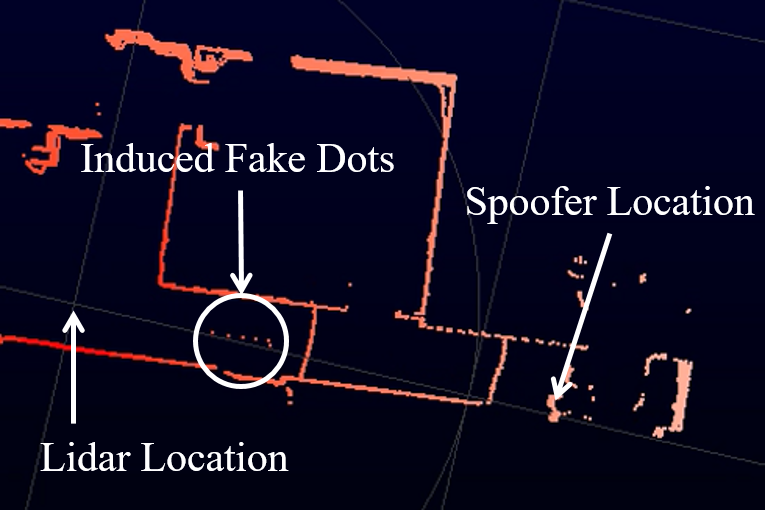
\includegraphics[width=\textwidth]{img/lidar/interference_distance_control.png}
	\caption{}%Spoofing an obstacle at a closer distance than the spoofer}
		\label{fig:shinInterferenceDistance}
	\end{subfigure}
	\caption[Spoofing obstacles on \ac{lidar} at different angles and closer distances that the spoofer.]{Spoofing examples on a Velodyne VLP-16 \ac{lidar}, extracted from Source~\cite{Shin2017}. Sub-Figure~(\subref{fig:shinInterferenceAngle}) shows the spoofed object at a different angle of the spoofer and sub-Figure~(\subref{fig:shinInterferenceDistance}) shows the spoofed object at a different distance than the spoofer.}
	\label{fig:shinInterference}
\end{figure}


\subsection{Two-Dimensional Coplanar \ac{lidar} Interference}
Gunzung Kim\etal, in 2015, presents the first results on multiple \ac{lidar} interference on their three papers~\cite{Kim2015a, Kim2015b, Kim2015c}. The three papers are based on a SICK LMS-511, a 2D \ac{lidar}\footnote{A single \ac{laser} and photodetector are mounted on a rotating device, measuring several azimuthal angles when the motor rotates, but the polar angle is kept fixed, scanning a single line of the environment.}. Kim\etal setups consist of a box with $\SI{5.3}{\meter} \times \SI{4}{\meter}$~\cite{Kim2015a} or $\SI{5.3}{\meter} \times \SI{5.3}{\meter}$~\cite{Kim2015b, Kim2015c}, with the \acp{lidar} positioned inside. The walls are made of a non-glossy wood and the experimental setup is shown in Figure~\ref{fig:kim-setups}. His classification of interference is based on the determination of a majorant and minorant for the distance of the wall, with a 10\% tolerance around the mean value.

\begin{figure}[!ht]
	\centering
	\begin{subfigure}[c]{0.45\textwidth}
		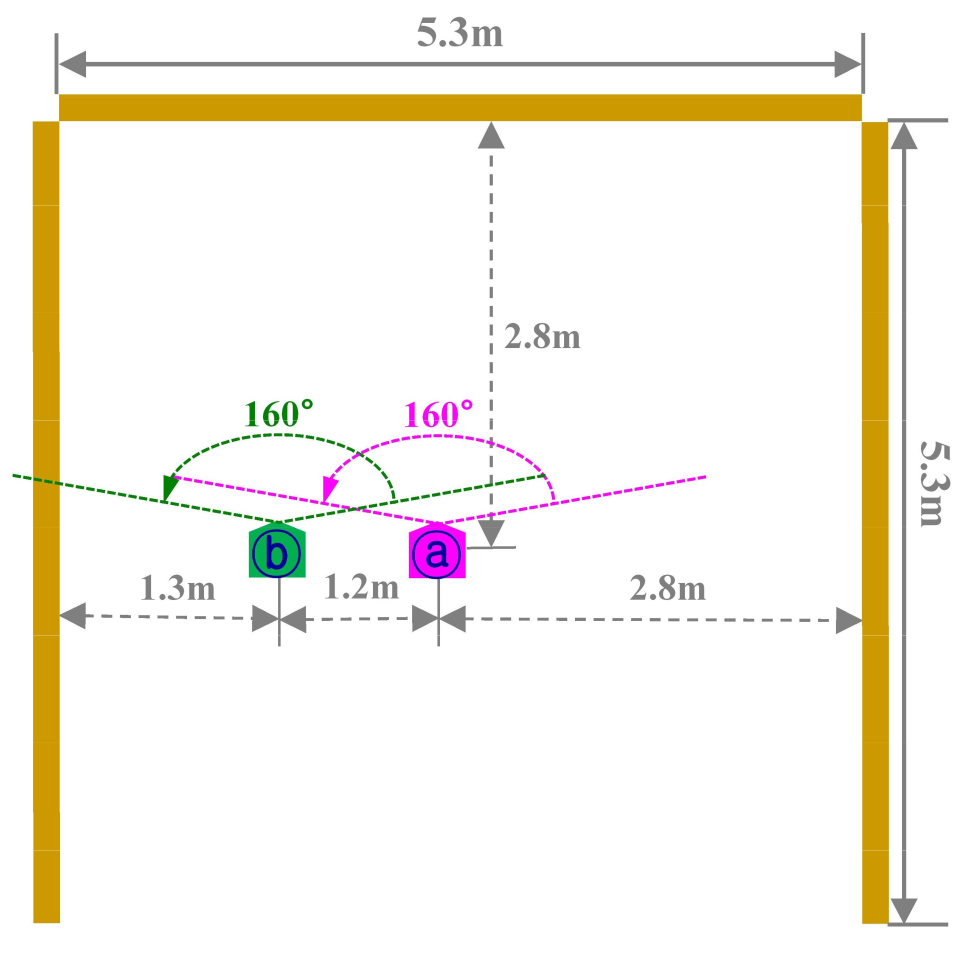
\includegraphics[width=\textwidth]{img/lidar-interference/kim-setup-side-by-side-1.png}
		\caption{\textit{Side-by-Side \#1}.}
		\label{fig:kim-side-by-side-1}
	\end{subfigure}
	\quad
	\begin{subfigure}[c]{0.45\textwidth}
		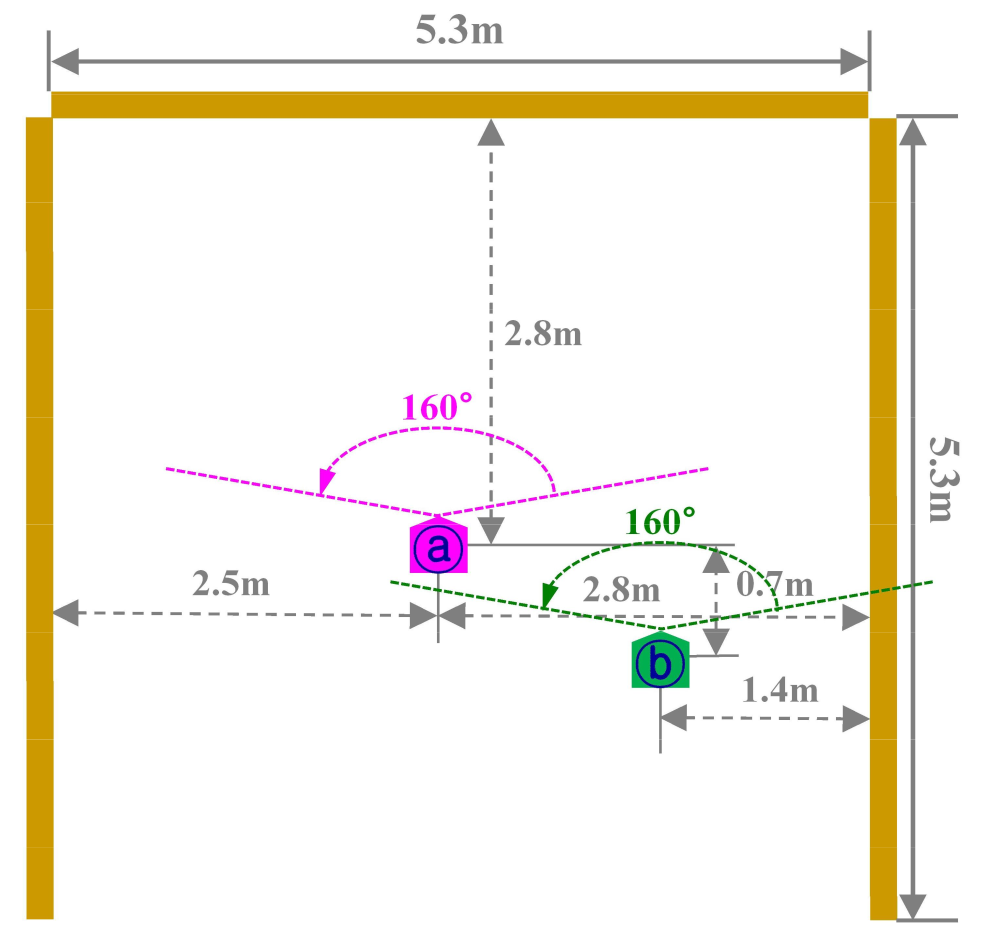
\includegraphics[width=\textwidth]{img/lidar-interference/kim-setup-side-by-side-2.png}
		\caption{\textit{Side-by-Side \#2}.}
		\label{fig:kim-side-by-side-2}
	\end{subfigure}
	\\ \vspace{4mm}
	\centering
	\begin{subfigure}[c]{0.45\textwidth}
		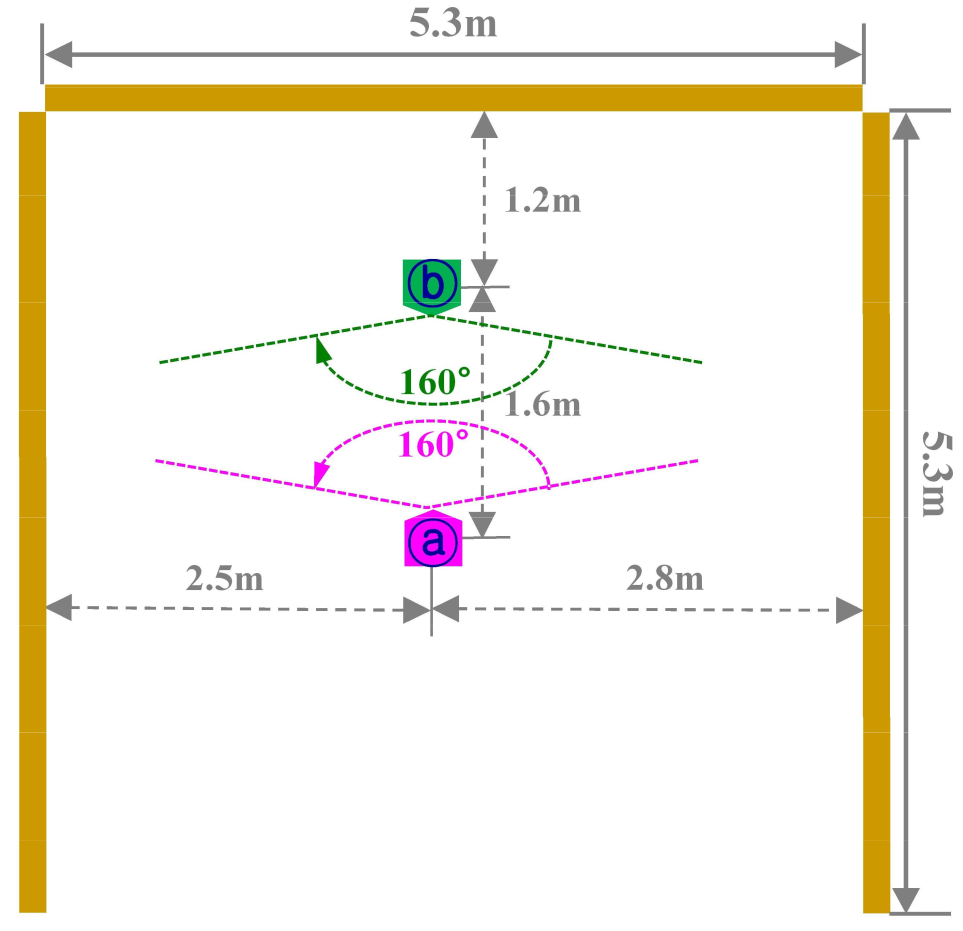
\includegraphics[width=\textwidth]{img/lidar-interference/kim-setup-face-to-face.png}
		\caption{\textit{Face-to-Face}.}
		\label{fig:kim-face-to-face}
	\end{subfigure}
	\quad
	\begin{subfigure}[c]{0.45\textwidth}
		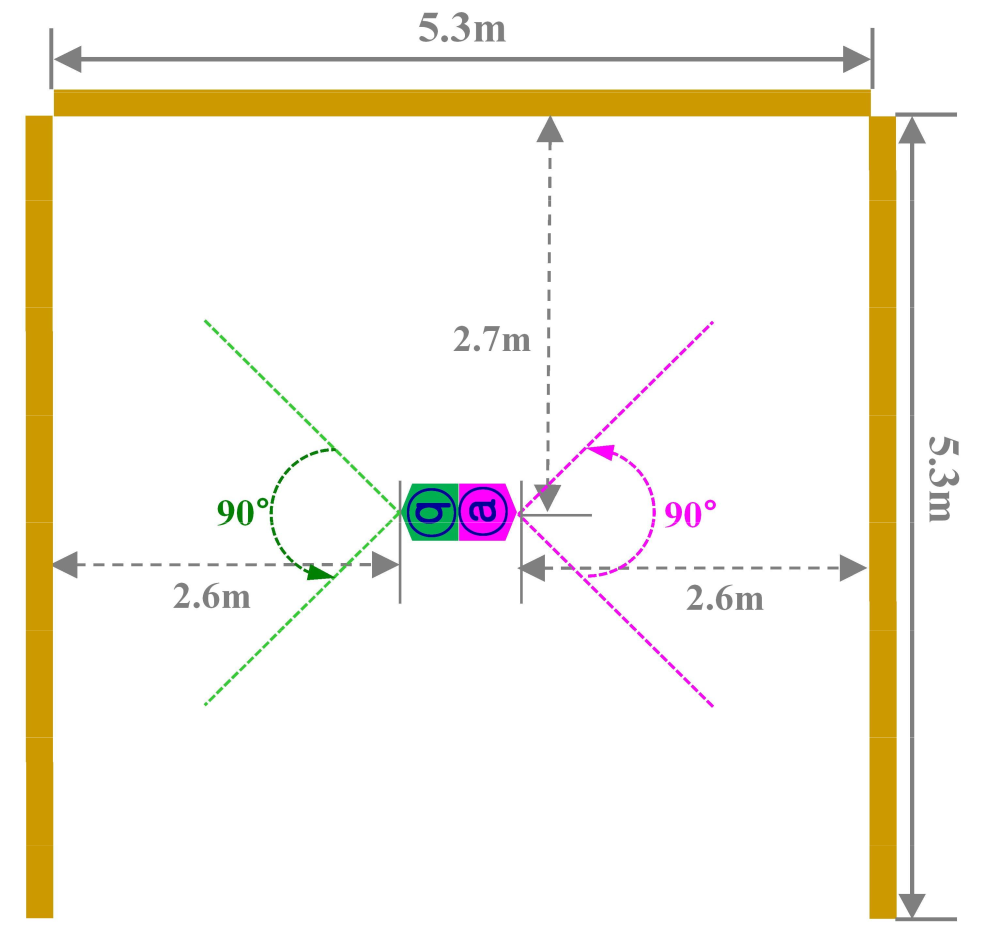
\includegraphics[width=\textwidth]{img/lidar-interference/kim-setup-back-to-back.png}
		\caption{\textit{Back-to-back}.}
		\label{fig:kim-back-to-back}
	\end{subfigure}

	\caption[Experimental setups used by Kim\etal and Popko\etal for 2D \ac{lidar} interference studies.]{Experimental setups devised by Gunzung Kim\etal, as detailed on~\cite{Kim2017}. Sub-Figure~(\subref{fig:kim-side-by-side-1}) and (\subref{fig:kim-side-by-side-2}) consist of an interference setup where the victim and interferer \ac{lidar} are adjacent to each other. Sub-Figure~(\subref{fig:kim-face-to-face}) tests the interference when the two \acp{lidar} are on each other \ac{fov} and sub-Figure~(\subref{fig:kim-back-to-back}) when the \acp{lidar} are not on each other \ac{fov}.}
	\label{fig:kim-setups}
\end{figure}


% Kim \etal research despite using a 2D \ac{lidar} instead of a 3D \ac{lidar} is the only study to use two independent 2D \ac{lidar}s interfering with each other. Kim \etal results indicate that interference has spatial and temporal locality \cite{Kim2015} and in any given time, in Kim's setup, a data point has 0.05 \% probability of being interfered \cite{Kim2015}. The former states that if a particular angle is interfered, the following angles are likely to also be interfered; while the latter indicates that if a measure is interfered, on the following frame that same measure is also likely to be interfered. 

Kim\etal tests show the temporal and spatial locality of the data. Temporal locality implies that a given angular direction is more likely to be interfered if it was interfered in the past, indicating that interference persists through time. Spatial locality implies that, for a current scan, if an interference occurs, it is more likely that the next angle will also be interfered, indicating that interference persists through space. 

The experiment conducted in~\cite{Kim2015a} captured a ground-truth model for 4 hours and the interference data for 50 hours. For a given angle position, Kim concluded that for his experimental setup, 4.4\% of the total number of full line scans were interfered, but that number only translates to one in every 2000 point (0.05\% interfered points for the total number of registered points). When considering the nature of interference, spatial interference is rare: 78\% of the interfered points are not interfered on their next measurement (against 15\% that are), and only 7\% of the angular positions are interfered consecutively 3 or more times, for a record of 13 (meaning \SI{0.5}{\second} of interference). For consecutive interference on nearby azimuthal angles on the same scan, only 30\% of the interference happens within single angular step and 26\% on a second. The largest consecutive number of angles with interference are 102, which translates to \SI{25.5}{\degree}.

In~\cite{Kim2015b}, Kim~\etal reports new tests on \ac{lidar} interference, adding two new tests: a side-by-side with a small displacement and a face-to-face test. In~\cite{Kim2015c} a back-to-back test is also performed. Note that despite the experimental setup \textit{Side by side \#1} (Figure~\ref{fig:kim-side-by-side-1}) being identical to the setup on~\cite{Kim2015a}, disagreements on all evaluated metrics occur. Therefore, for this test, the results discussed before, taken from~\cite{Kim2015a}, and results presented in Table~\ref{tab:kim_2015_results}, based on~\cite{Kim2015b, Kim2015c}, are not in agreement. No explanations are provided for such difference and the issue is not addressed by Kim\etal on~\cite{Kim2015b, Kim2015c}.

\begin{table}[!ht]
	\centering
	\renewcommand{\arraystretch}{1.3}
	\begin{tabular}{@{}p{3.5cm}C{3cm}C{4cm}@{}}
			\toprule
			Experimental Setup Codename & \% of Lines Interfered & Relative Frequence of Interfered Points \\
			\midrule
			Side-by-side \#1 & $1.795$                & $3.103\E^{-5}$  \\
			Side-by-side \#2 & $10.33$                & $1.667\E^{-4}$ \\ \midrule
			Face-to-Face     & $1.433$                & $2.583\E^{-5}$  \\ \midrule
			Back-to-Back A   & $0.211$                & $3.387\E^{-6}$  \\
			Back-to-Back B   & $0.216$                & $3.514\E^{-6}$  \\ \bottomrule
		\end{tabular}
		\caption[Summary of Kim's\etal \ac{lidar} interference results.]{Summary of Kim's\etal the interference results from~\cite{Kim2015b, Kim2015c}, for all tests. In the second column, the percentage of lines with a single interfered point are presented. The third column corresponds to the relative frequency of interfered point for all the points.}
	\label{tab:kim_2015_results}
\end{table}

The results of the second column, \textit{\% of Lines Interfered}, characterizes the number of lines on which interference as been found. For every test scenario on this column, the line interference caused are mostly non-consecutive (above 90\% for Face to Face and 94.3\% for all the other tests).

The third column, \textit{Relative Frequence of Interfered Points}, characterizes the number of points that have been interfered regarding all points taken. The relative frequency of the interference is low, with the relation between the interfered and the total number of points being on the order of magnitude of $10^{-6}$ to $10^{-4}$. Despite the maximum of consecutive spatial interference (4 scans), more than $99.7\%$ of all interferences happen isolated on a given azimuth angle, with no repetition on the next scan for the same interfered angle~\cite{Kim2015c}. 



% To the best of the author's knowledge, despite the relevance of the topic to a society of self-driving cars, there are only three different studies available


In 2017, Kim\etal present the results on the above papers~\cite{Kim2015a, Kim2015b, Kim2015c}, extending its research by performing an intensity analysis~\cite{Kim2017}. His findings are that on a mutual interference scenario, the intensity of the received \ac{laser} pulses varies significantly, confirming Hebert and Krotkov early findings that on a \ac{lidar} system range and intensity measures are not completely independent and interfering with one affects the results of other~\cite{Hebert}.

In the same paper, he also introduces a theoretical analysis of the multipath interference based on a Lambertian distribution for modelling the reflections on the walls~\cite{Kim2017}. The model lacks generality, as it assumes average values for several parameters and some simplifications on the multipath interference, but allows to conclude that:

\begin{enumerate}
	\item After the second reflection on an obstacle, the attenuation suffered by the light beam is not sufficient for the receiving \ac{lidar} to detect it as an interference;
	\item Direct interference (on Kim's experimental setup and hardware) is likely to saturate the receiver of the interfered \ac{lidar}, which may or may not be considered a valid measurement by the hardware;
	\item Indirect interference with only one reflection can be interpreted as a valid measurement, since the intensity of the received interfered beam is similar to the intensity of a valid measurement beam.
\end{enumerate}

In 2019, Gerald Popko\etal~\cite{Popko2019a} presents a mathematical description on how stationary, coplanar and circular 2D scanning \ac{lidar} can interfere through beam path interference of the optical \ac{fov}. Based on his description, he repeats Kim's\etal experiments (see Figure~\ref{fig:kim-setups}), proposing a new statistical interference detector, instead of Kim's maximum distance minorant and majorant~\cite{Kim2015a}, and also performs a Monte-Carlo simulation~\cite{Popko2019b}. Popko\etal findings are that:

\begin{enumerate}
	\item The interference behavior depends majorly on the target geometry and beam intersection, and not on radiometric considerations;
	\item Simulating the \ac{lidar} interference is not yet reliable, since for the model developed only the scattered interference provided a value close to the real value measured;
	\item The direct interference is dominant over the scattering interference;
	\item The direct interference is mainly responsible for small distance measurement errors, while scattering interference is mainly present for large distance measurement errors.
\end{enumerate}

Lastly, Popko \etal interference results are two orders of magnitude higher than Kim's \etal measurements, $1.041 \%$~\cite{Popko2019b} vs $0.05\%$~\cite{Kim2015a}.

\subsection{A departing note on \ac{lidar} interference}
On a departing note, \ac{tof} \ac{lidar} is the mainstream \ac{lidar} for autonomous vehicles and the automotive industry, while being the less robust to crosstalk from other \ac{tof} \acp{lidar}. So far, the studies presented on \ac{lidar} interference are scarce and not representative, focused only on two-dimensional \acp{lidar}, i.e., \acp{lidar} that only scan a single line. Answers about the relevance of \ac{lidar} interference are yet to be given and more tests are required, to fully profile the interference and its impacts on autonomous driving. Robust alternatives to crosstalk, both from a technological and signal processing standpoint are also desirable.

%\chapter{Camera and \acs{lidar} Calibration}
\label{chapter:calibration}

The focus of this chapter is to detail the considerations and procedures used on sensory calibration, starting by describing the experimental setup. Then, the method used to calibrate the camera and \ac{lidar} intrinsic parameters are detailed and results are shown. After properly intrinsic calibration, the two sensors can be calibrated amongst themselves, through an extrinsic calibration procedure. This procedure is explained from a mathematical standpoint and the implementation is here detailed, along with results.


\section{Experimental Setup}
\label{sec:calibration:experimental-setup}
The experimental setup is shown on Figure~\ref{fig:experimental-setup}. It consists of an industrial camera with an objective lens, a \ac{tof} \ac{lidar}, an Ethernet switch and a power source (not shown on the figure). The setup is constructed using Thorlabs\cp~Optomechanic material to mount the camera and \ac{lidar}.

\begin{figure}[!ht]
	\centering
	\begin{subfigure}[c]{0.45\textwidth}
		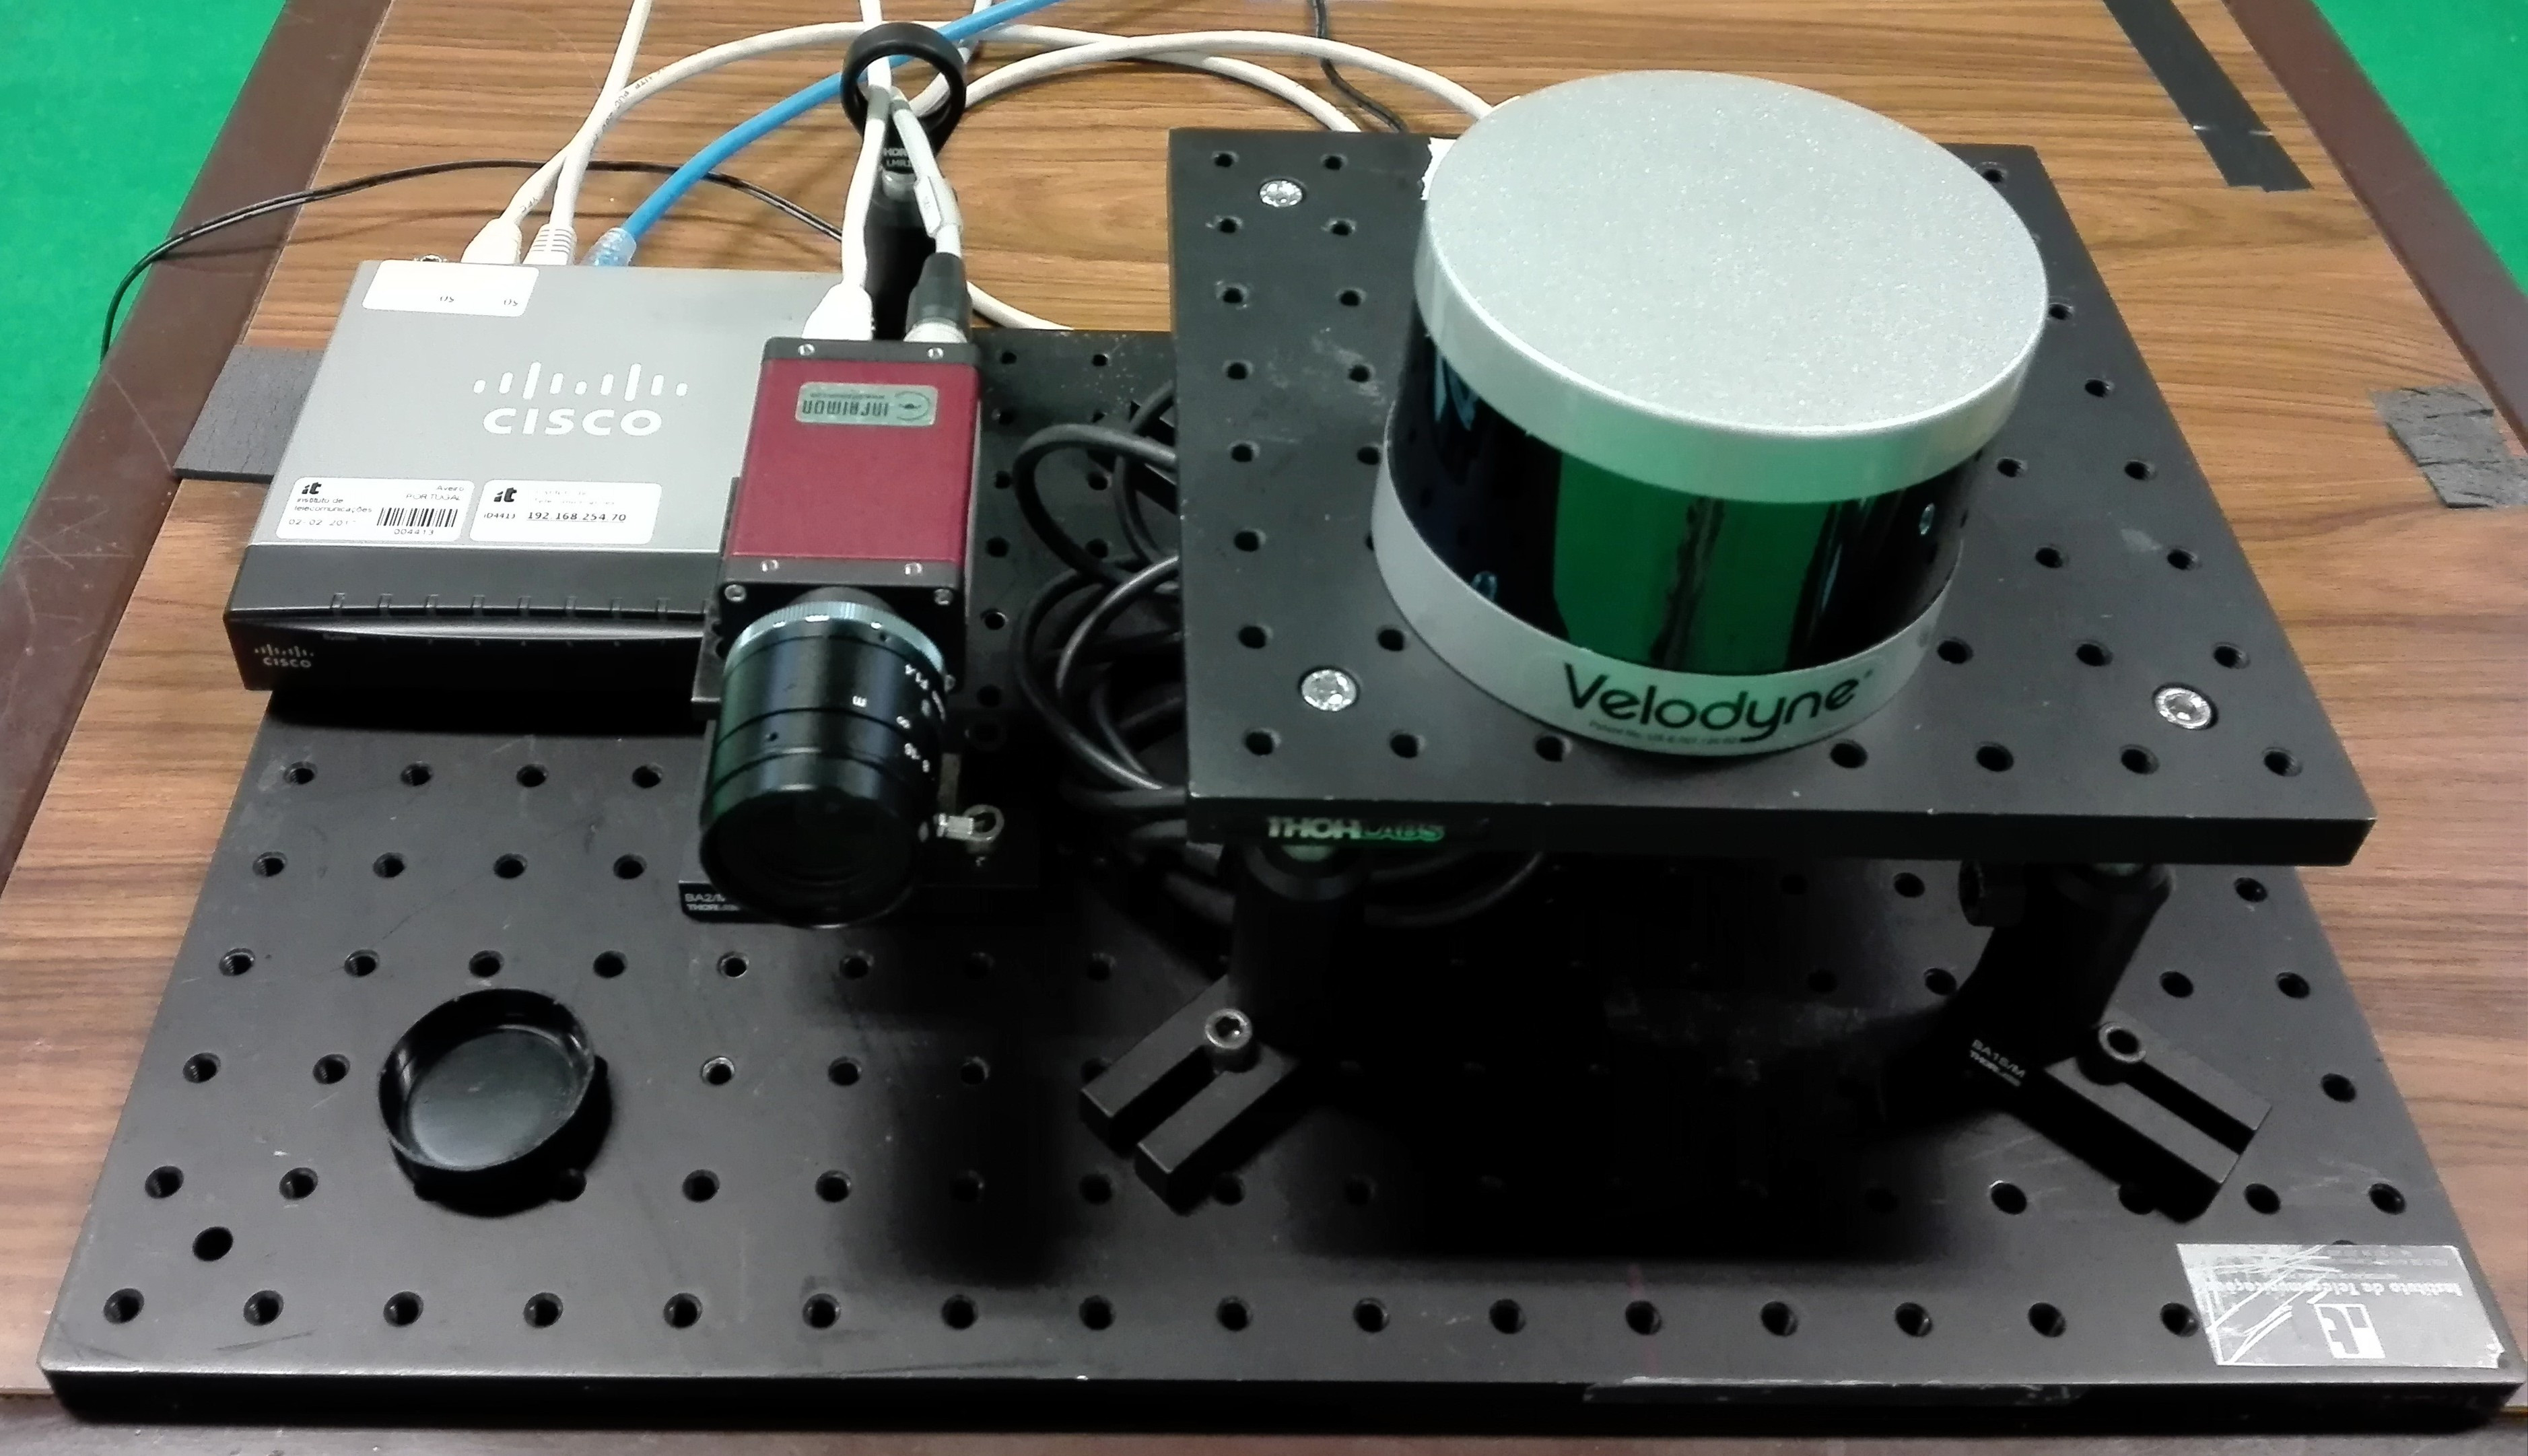
\includegraphics[width=\textwidth]{img/experimental-setup/table-setup-cambada-perspective.jpg}
		\caption{}
		\label{fig:experimental-setup:perspective}
	\end{subfigure}
	\qquad
	\begin{subfigure}[c]{0.45\textwidth}
		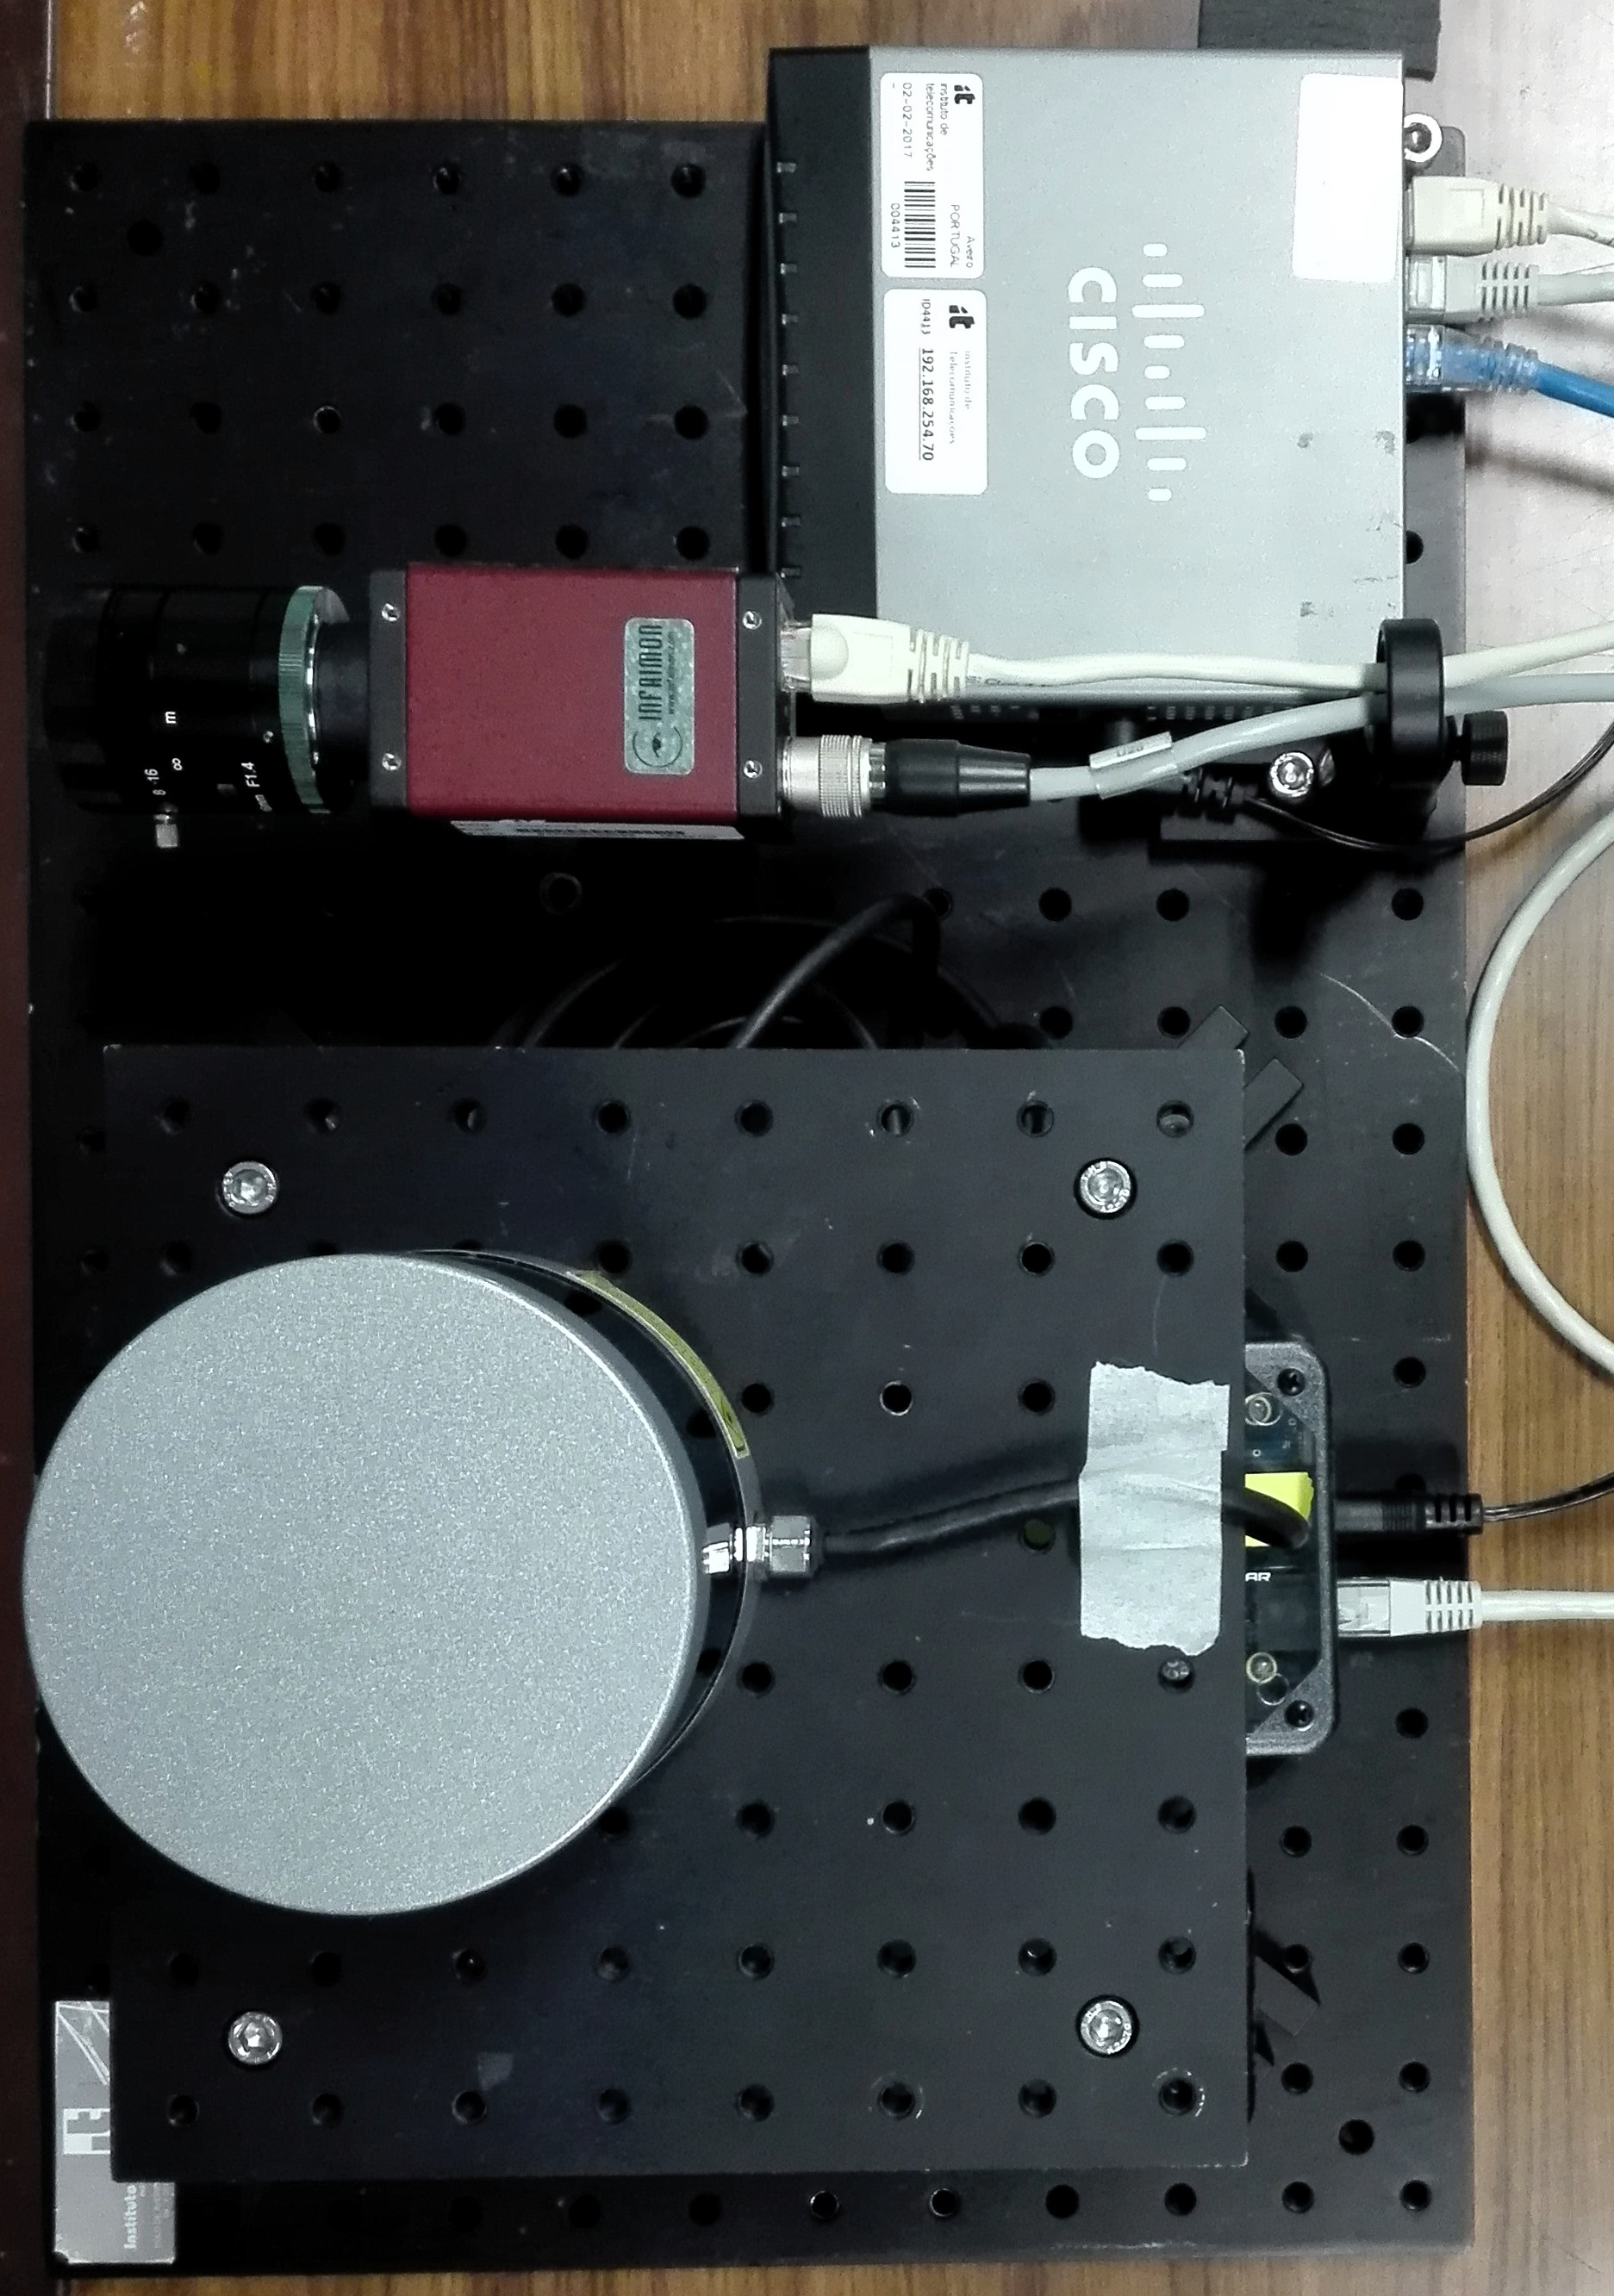
\includegraphics[width=0.65\textwidth, keepaspectratio, angle=90]{img/experimental-setup/table-setup-cambada-birds-eye.jpg}
		\caption{}
		\label{fig:experimental-setup:birds-eye}
	\end{subfigure}
	\caption[Perspective and top views of the experimental setup for the camera and \acs{lidar}.]{Relative positioning of the devices on the experimental. The \ac{lidar} is on an elevated platform to guarantee that the camera and Ethernet switch are not on its \ac{fov}. Sub-figures show the experimental setup viewed (\subref{fig:experimental-setup:perspective}) in perspective; (\subref{fig:experimental-setup:birds-eye}) from the top.}
	\label{fig:experimental-setup}
\end{figure}

\subsection{Camera and Lens}
The camera used is an industrial 5 \ac{mp} RGB camera, from \acf{avt}, model Manta G-504C. The objective is a C-Mount lens with lock from Thorlabs\cp, model MVL16M1. The full camera specifications can be accessed on~\cite{MantaG504C} and the full lens specifications on~\cite{Thorlabs}. Relevant specifications of the camera and lens are summarized  on Table~\ref{tab:camera-and-lens-specs}. 

\begin{table}[!ht]
	\renewcommand{\arraystretch}{1.2}
	\centering
	\begin{tabular}{@{}lp{7cm}l@{}}
		\toprule
		\multicolumn{2}{l}{Specification} & Value \\ \midrule
		\multicolumn{2}{l}{\emph{Camera}} & \\
		\phantom{a} & Full Resolution (width vs height) & $2452 \times 2056$ pixels \\
									& Shutter mode & Global \\
									&	Maximum \ac{fps} at full resolution & $9.2$ \\ 
									& \acs{adc}\footnotemark bit depth & $12$ bit \\\midrule 
									\multicolumn{2}{l}{\emph{Lens}} \\
									&	Focal Length & $16$ mm \\
									&	Max aperture & $f/1.4$ \\
									&	Minimum Object Distance & $300$ mm  \\
		\bottomrule
	\end{tabular}
	\caption[Relevant specifications of the camera and its lens.]{Relevant specifications for \ac{avt} Manta G-504C RGB camera (from~\cite{MantaG504C})  and MVL16M1 Thorlabs\cp~lens (from~\cite{Thorlabs}).}
	\label{tab:camera-and-lens-specs}
\end{table}

\footnotetext{\acs{adc} stands for \acl{adc}}

To power the Manta G-504C, a benchtop power source was used. Further details about powering the camera and its electrical connections are presented on Appendix-B~\ref{sec:appendix-b}.

\subsection{\ac{tof} \ac{lidar}}
The \ac{tof} \ac{lidar} used is a Velodyne VLP-16\texttrademark, a 16 beam \ac{lidar} that operates with a wavelength of \SI{903}{\nano\meter}. VLP-16 supports various measurements modes based on the return pulse (Strongest, Last, Dual) and can be connected to a \ac{gps} receiver for geopositioning and synchronization with an external clock. It also supports several rotation speeds, from 300 to 1200 \ac{rpm}, which result in different angular steps and point cloud refresh rate. The full specifications can be accessed on~\cite{VLP16} and the relevant specifications for this work are summarized on Table~\ref{tab:vlp16-specs}.

\begin{table}[!ht]
	\renewcommand{\arraystretch}{1.2}
	\centering
	\begin{tabular}{@{}p{8.3cm}l@{}}
		\toprule
		Specification & Value \\ \midrule
		Wavelength    & \SI{903}{\nano\meter} \\
		Motor \acs{rpm} & $600 \pm 3$ \\
		Angular step & \SI{0.2}{\degree} \\
		Vertical \ac{fov} & \SI{30}{\degree} \\
		Horizontal \ac{fov} & \SI{360}{\degree} \\
		Maximum Scanning Distance & \SI{100}{\meter} \\
		Theoretical Typical Distance Error & \SI{2}{\centi\meter} \\
		\bottomrule
	\end{tabular}
	\caption[Velodyne\cp~VLP-16 relevant\texttrademark relevant specifications.]{Velodyne VLP-16 relevant specifications. Source~\cite{VLP16}.}
	\label{tab:vlp16-specs}
\end{table}


\subsection{Connection Setup} 
Both Velodyne VLP-16 and \ac{avt} Manta G-504C operate over Gigabit Ethernet. Therefore, a Gigabit  Ethernet switch is required to connect all the equipment to a single computer using a single Ethernet port. The switch used was Cisco SG200-08, an 8-Port Gigabit Smart Switch. 

The switch was configured so that every port was on the same \ac{vlan}, ensuring packets were accessible on the computer, since the sensors were configured to broadcast the packets. An alternative to this implementation was to redirect the packets from each sensor to the computer network and filter the packets from the computer to the sensors, by putting them on separated networks and create a network traffic management solution. Using \ac{ros} capabilities to measure packet delay and rate of publishing of the data messages, no bandwidth constraints or packet delay/loss were verified. Therefore, the solution chosen was the former, due to its simplicity. 

For each device a fixed \acf{ip} address was attributed, following the instructions on their datasheet~\cite{VLP16, MantaVision2013}. The \ac{ip} addresses can be consulted on Table~\ref{tab:experimental-setup-ip}.

\begin{table}[!ht]
	\renewcommand{\arraystretch}{1.2}
	\centering
	\begin{tabular}{@{}lcc@{}}
		\toprule
		Device          & \ac{ip} Address & Subnet Mask\\ \midrule
		Computer        & 192.168.10.77  & 255.255.255.0 \\
		Manta G-504C    & 192.168.10.1   & 255.255.255.0 \\
		Velodyne VLP-16 & 192.168.10.201 & 255.255.255.0 \\
		\bottomrule
	\end{tabular}
	\caption[\acs{ip} addresses and subnet masks for the devices connected on the experimental setup.]{\ac{ip} addresses and subnet masks for the devices connected on the experimental setup.}
	\label{tab:experimental-setup-ip}
\end{table}

\subsection{\ac{lidar} and Camera Interference}
No significant interference is expected between the camera and the \ac{lidar}. Despite the camera lens having a transmission coefficient of $66\%$ at $\approx 900 nm$~\cite{Thorlabs}, and Sony ICX655, the camera sensor for the \ac{avt} Manta G-504C, having a Quantum Efficiency of $\approx 5\%$~\cite{MantaG504C}, \ac{avt} Manta G-504C is equipped with an \ac{ir} cut-filter.

Despite the low sensibility of the camera and the presence of an \ac{ir} cut-filter, an experiment was conducted to verify the occurrence of interference. The experimental setup was switched on in a Dark Room without any other light sources and the camera feed was visualized. Besides the noise caused by the camera electronics operation, no signs of interference caused by the \ac{lidar} infrared beams could be observed on the camera image feed, since no bright spots were found. Therefore, no further work on \ac{lidar} to camera interference were carried


%\begin{figure}[H]
%	\centering
%	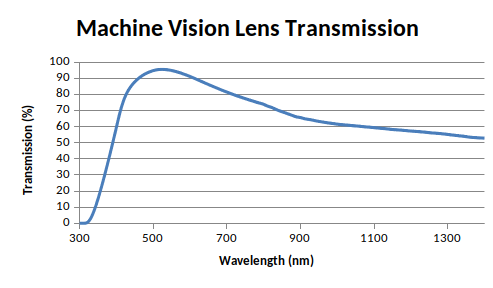
\includegraphics[width=0.6\textwidth]{img/experimental-setup/lens-transmission.png}
%	\caption{Transmission of the MVL16M1 lens in relation the light wavelength. Source~\cite{Thorlabs}}
%	\label{fig:lens-transmission}
%\end{figure}



\section{Camera Intrinsic Calibration}
\label{sec:calibration:camera}
The act of calibrating a camera consists on determining its intrinsic parameters, as detailed in sub-Section~\ref{subsec:sota:camera-intrinisc-calibration}. This can be done by taking different images with a known pattern, fully visible on the camera \ac{fov}, changing its rotation and translation in relation to the camera coordinate frame.

The calibration procedure undertaken uses a chessboard of $13 \times 9$ squares, with each square having an edge length of \SI{44.0}{\milli\meter}. The chessboard used can be seen on Figure~\ref{fig:chessboard}. It was laser printed on a \SI{100}{\gram} A2 paper and then glued to a plywood board.

\begin{figure}[H]
	\centering
	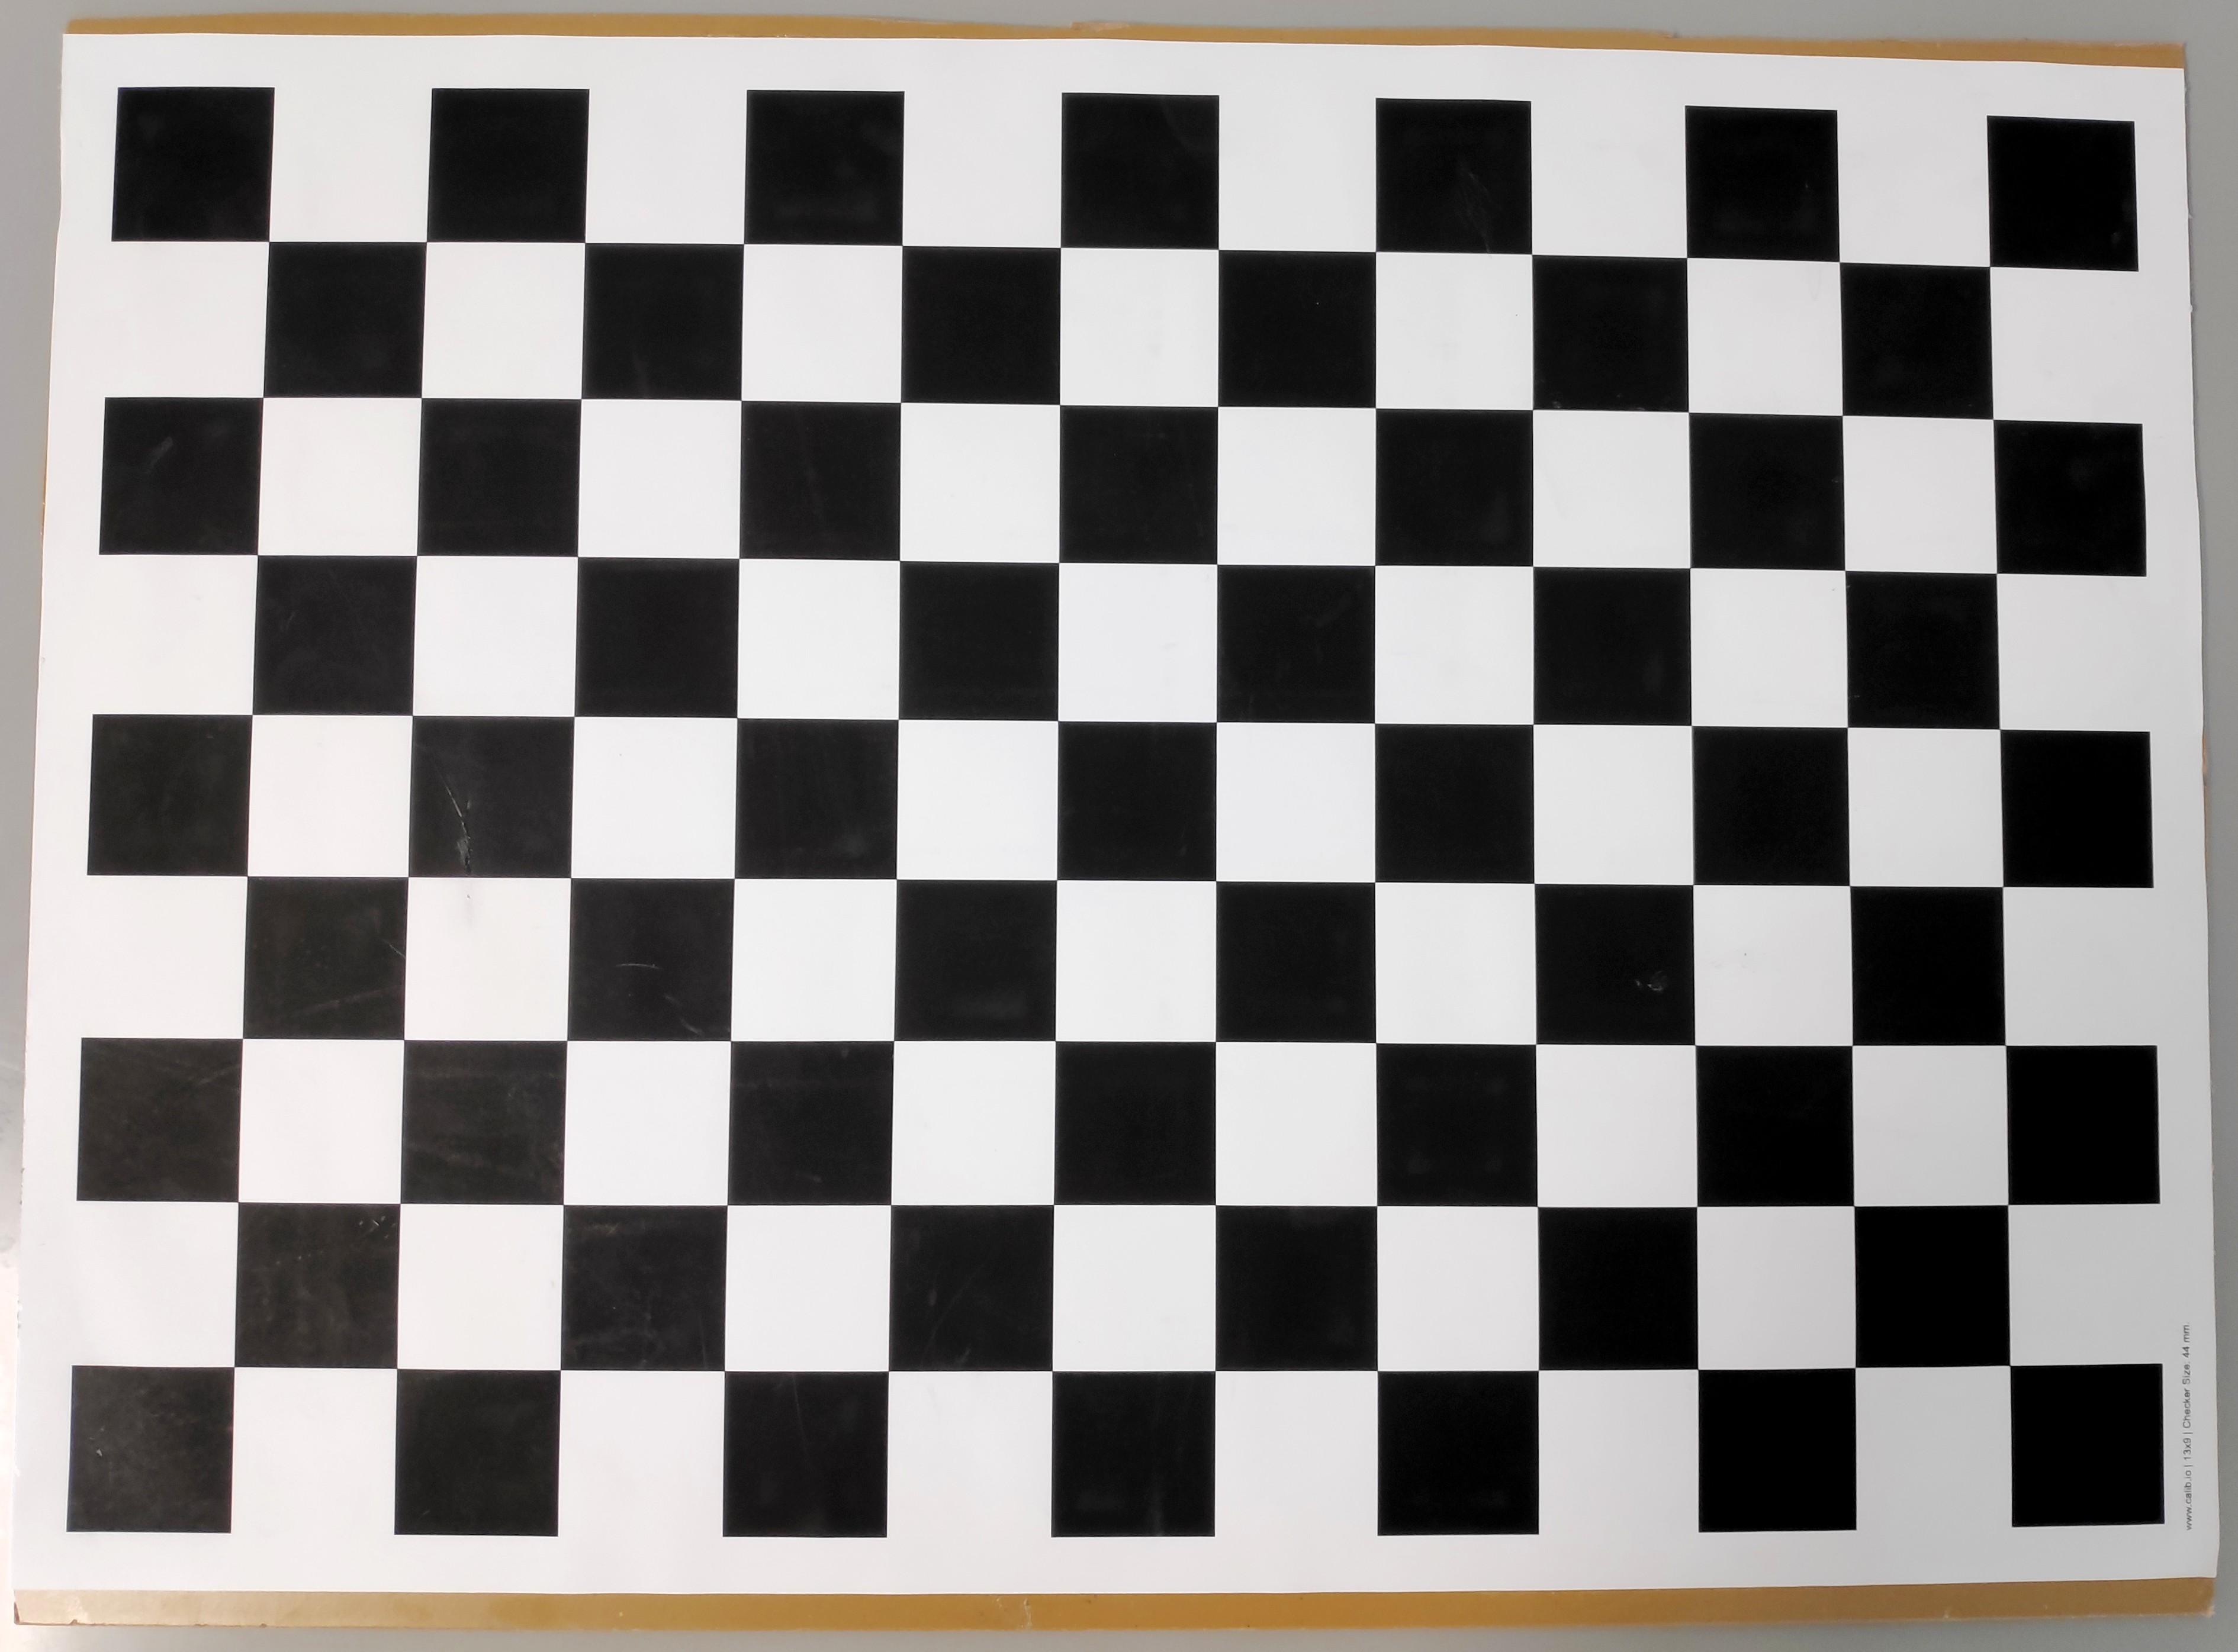
\includegraphics[width=0.5\textwidth]{img/experimental-setup/chessboard.jpg}
	\caption{Chessboard used during camera calibration procedures. The chessboard was laser printed on A2 paper size, in real size, that was then glued to a plywood board.}
	\label{fig:chessboard}
\end{figure}

Calibrating the camera requires that the calibration object to be focused. Therefore, before any proper calibration can be made, focus theory and procedure are given on the next sub-section,~\ref{subsec:calibration:camera-focus}.


\subsection{Camera Focus and \acl{dof}}
\label{subsec:calibration:camera-focus}
Focusing a camera can only be attained for an exact distance from the camera~\cite{Merklinger1993, Photopillers}, measured perpendicularly to the plane of focus, which is the plane containing the \ac{cmos} or \ac{ccd} chip. Therefore, on every image, there is a plane of focus and what actually ``looks focused'' is really just in ``acceptably sharp focus''.

``Acceptably sharp focus'' means that a point in the real world would not result in a point on the image (as happens in precise focus), but in a blurred spot~\cite{Photopillers}. However, if the size of blur is small enough, little to no differences can be perceived and the image is considered to be focused~\cite{Photopillers}. The maximum size at which this blur is not noticed by the viewer (given a specific sensor size, dimension of the viewed photo, viewing distance and acuity of the viewer) is when the \ac{coc} is smaller than the pixel size~\cite{Photopillers, Merklinger1993}.

The first step in focusing an image requires the calculation of the hyperfocal distance, $H$, the distance at which the camera is focused to ensure objects from half of this distance to the infinity are in an ``acceptably sharp focus'' (referred to as just focus, from now on). This distance can be calculated using the equation~\eqref{eq:hyperfocal_distance}, below, where $f$ is the focal length, $F_N$ is the F-number and $c$ the \ac{coc} limit. Hyperfocal near limit is defined as $H_\text{near} = \rfrac{H}{2}$.

\begin{equation}
	\label{eq:hyperfocal_distance}
	H = \frac{f^2}{F_Nc} + f \approx \frac{f^2}{F_Nc} 
\end{equation}

Known the hyperfocal distance, the \acf{dof} can be calculated. \ac{dof} is measured in meters and is obtained by subtracting the farthest and nearest distances at which an object is focused (see Equation~\eqref{eq:dof}), indicating the distance between this two points~\cite{Photopillers, Merklinger1993, mvg_book}. The nearest and farthest points can be calculated using the equations~\eqref{eq:dof-near} and~\eqref{eq:dof-far}, respectively, where $d$ is the target object distance to the camera sensor.

\begin{subequations}
	\label{eq:dof_all}
	\begin{align}
		DoF & = DoF_{far} - DoF_{near} \label{eq:dof} \\
		DoF_{far} & = \frac{H\times d}{H - (d - f)} \label{eq:dof-far} \\
		DoF_{near} & = \frac{H\times d}{H + (d - f)} \label{eq:dof-near} 
	\end{align}
\end{subequations}

Equations~\eqref{eq:dof_all} make it possible to select a desired \acl{dof} for an image that guarantees that all the objects of interest are focused. Taking in consideration that smaller apertures (bigger F-numbers) will increase the exposition time~\cite{Merklinger1993} (since the amount of light illuminating the sensor will be lower), a target distance can be selected with the guarantee that all the objects from the near \ac{dof} point to the far \ac{dof} will be sharp.

Rewriting the Equation~\eqref{eq:dof-near} to calculate the objects distance, giving the minimum distance at the objects must be focused, one gets: %the Equation~\eqref{eq:dof-subject-distance}.

\begin{equation}
	\label{eq:dof-subject-distance}
	d = \frac{(H - f) \cdot DoF_{near}}{H - DoF_{near}}
\end{equation}


\subsection{Camera Calibration Procedure}
For calibration, \ac{opencv} algorithms are used~\cite{opencv_doc}, such as \texttt{calibrateCamera}, \texttt{solvePnP} and \texttt{findChessboardCorners}. These algorithms, the underlying code interconnecting them and a \ac{gui} for performing calibration are available in a \ac{ros} package, \texttt{camera\_calibration} from the \texttt{image\_pipeline} metapackage~\cite{cameraCalibrationRos}, which we use for intrinsic camera calibration.

For calibration, around 50 unique photos are taken for each setup. These images are converted to greyscale, the chessboard corners are detected and the camera intrinsic parameters are computed by the \texttt{camera\_calibration} ROS package. A subset of the calibration images is presented on Figure~\ref{fig:camera-calibration-images}.

\begin{figure}[!ht]
	\centering
	\begin{subfigure}[c]{0.30\textwidth}
		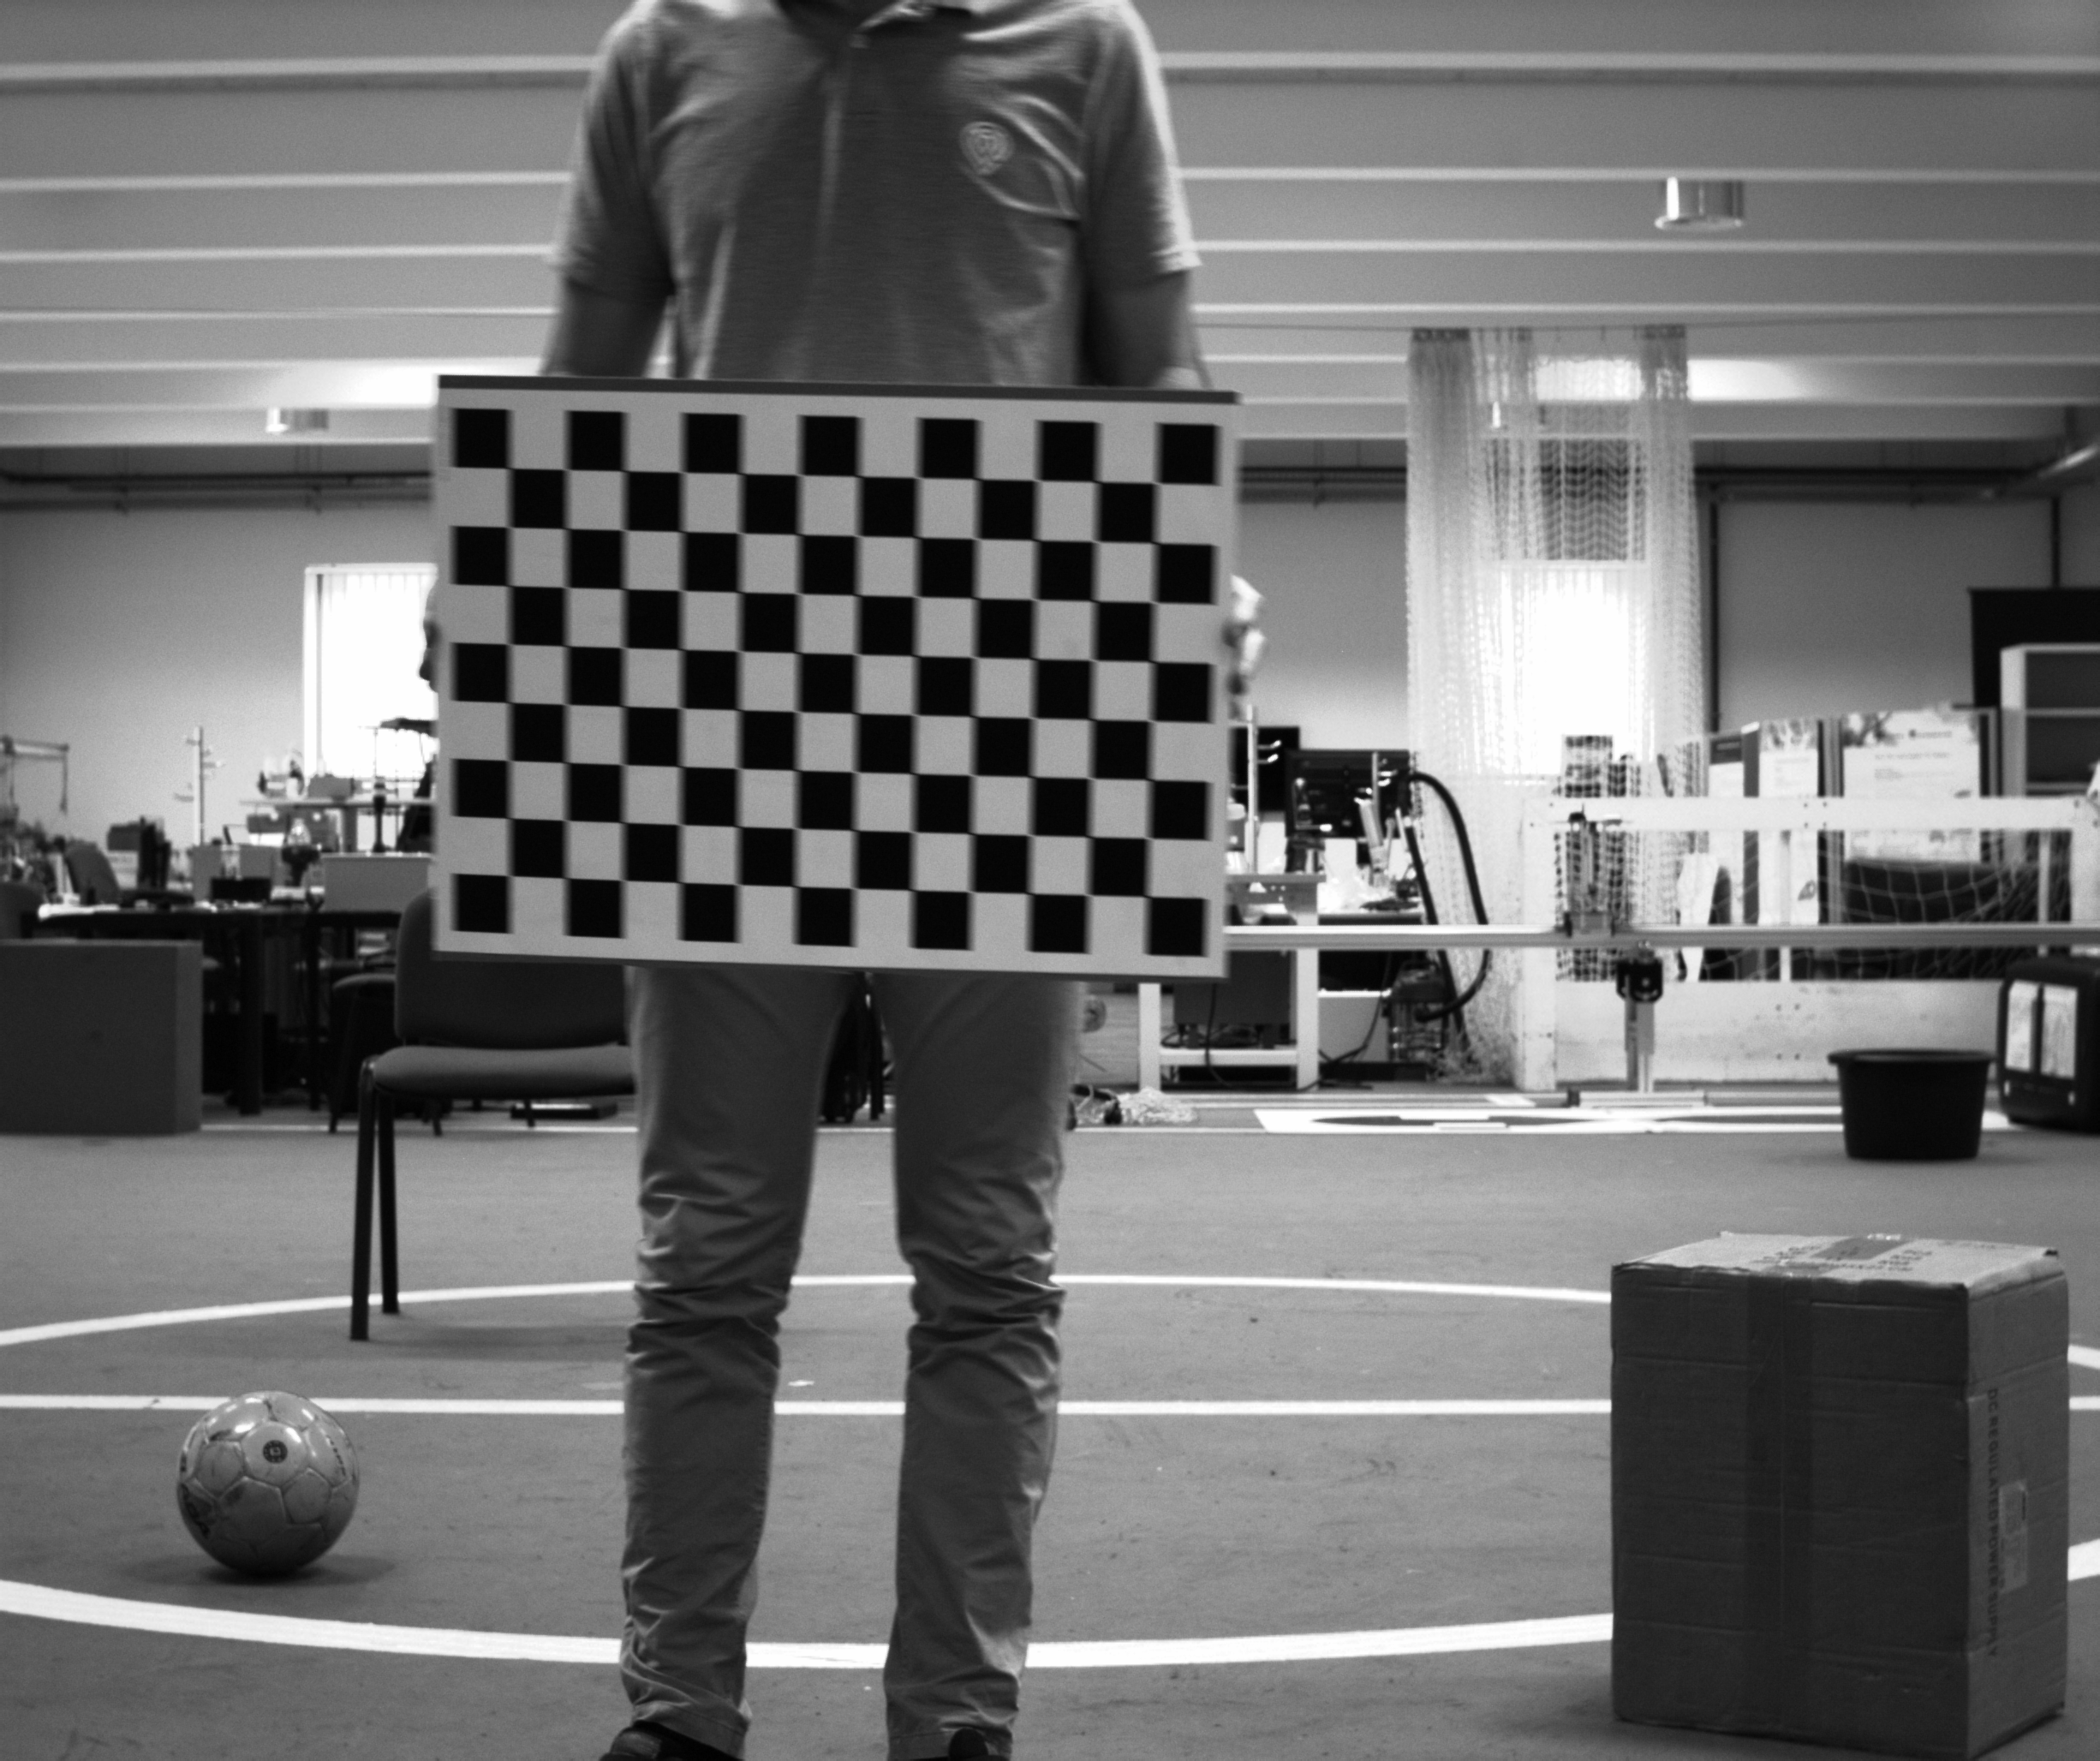
\includegraphics[width=0.9\textwidth]{img/camera-calibration/left-0001.png}
	\end{subfigure}
	\begin{subfigure}[c]{0.30\textwidth}
		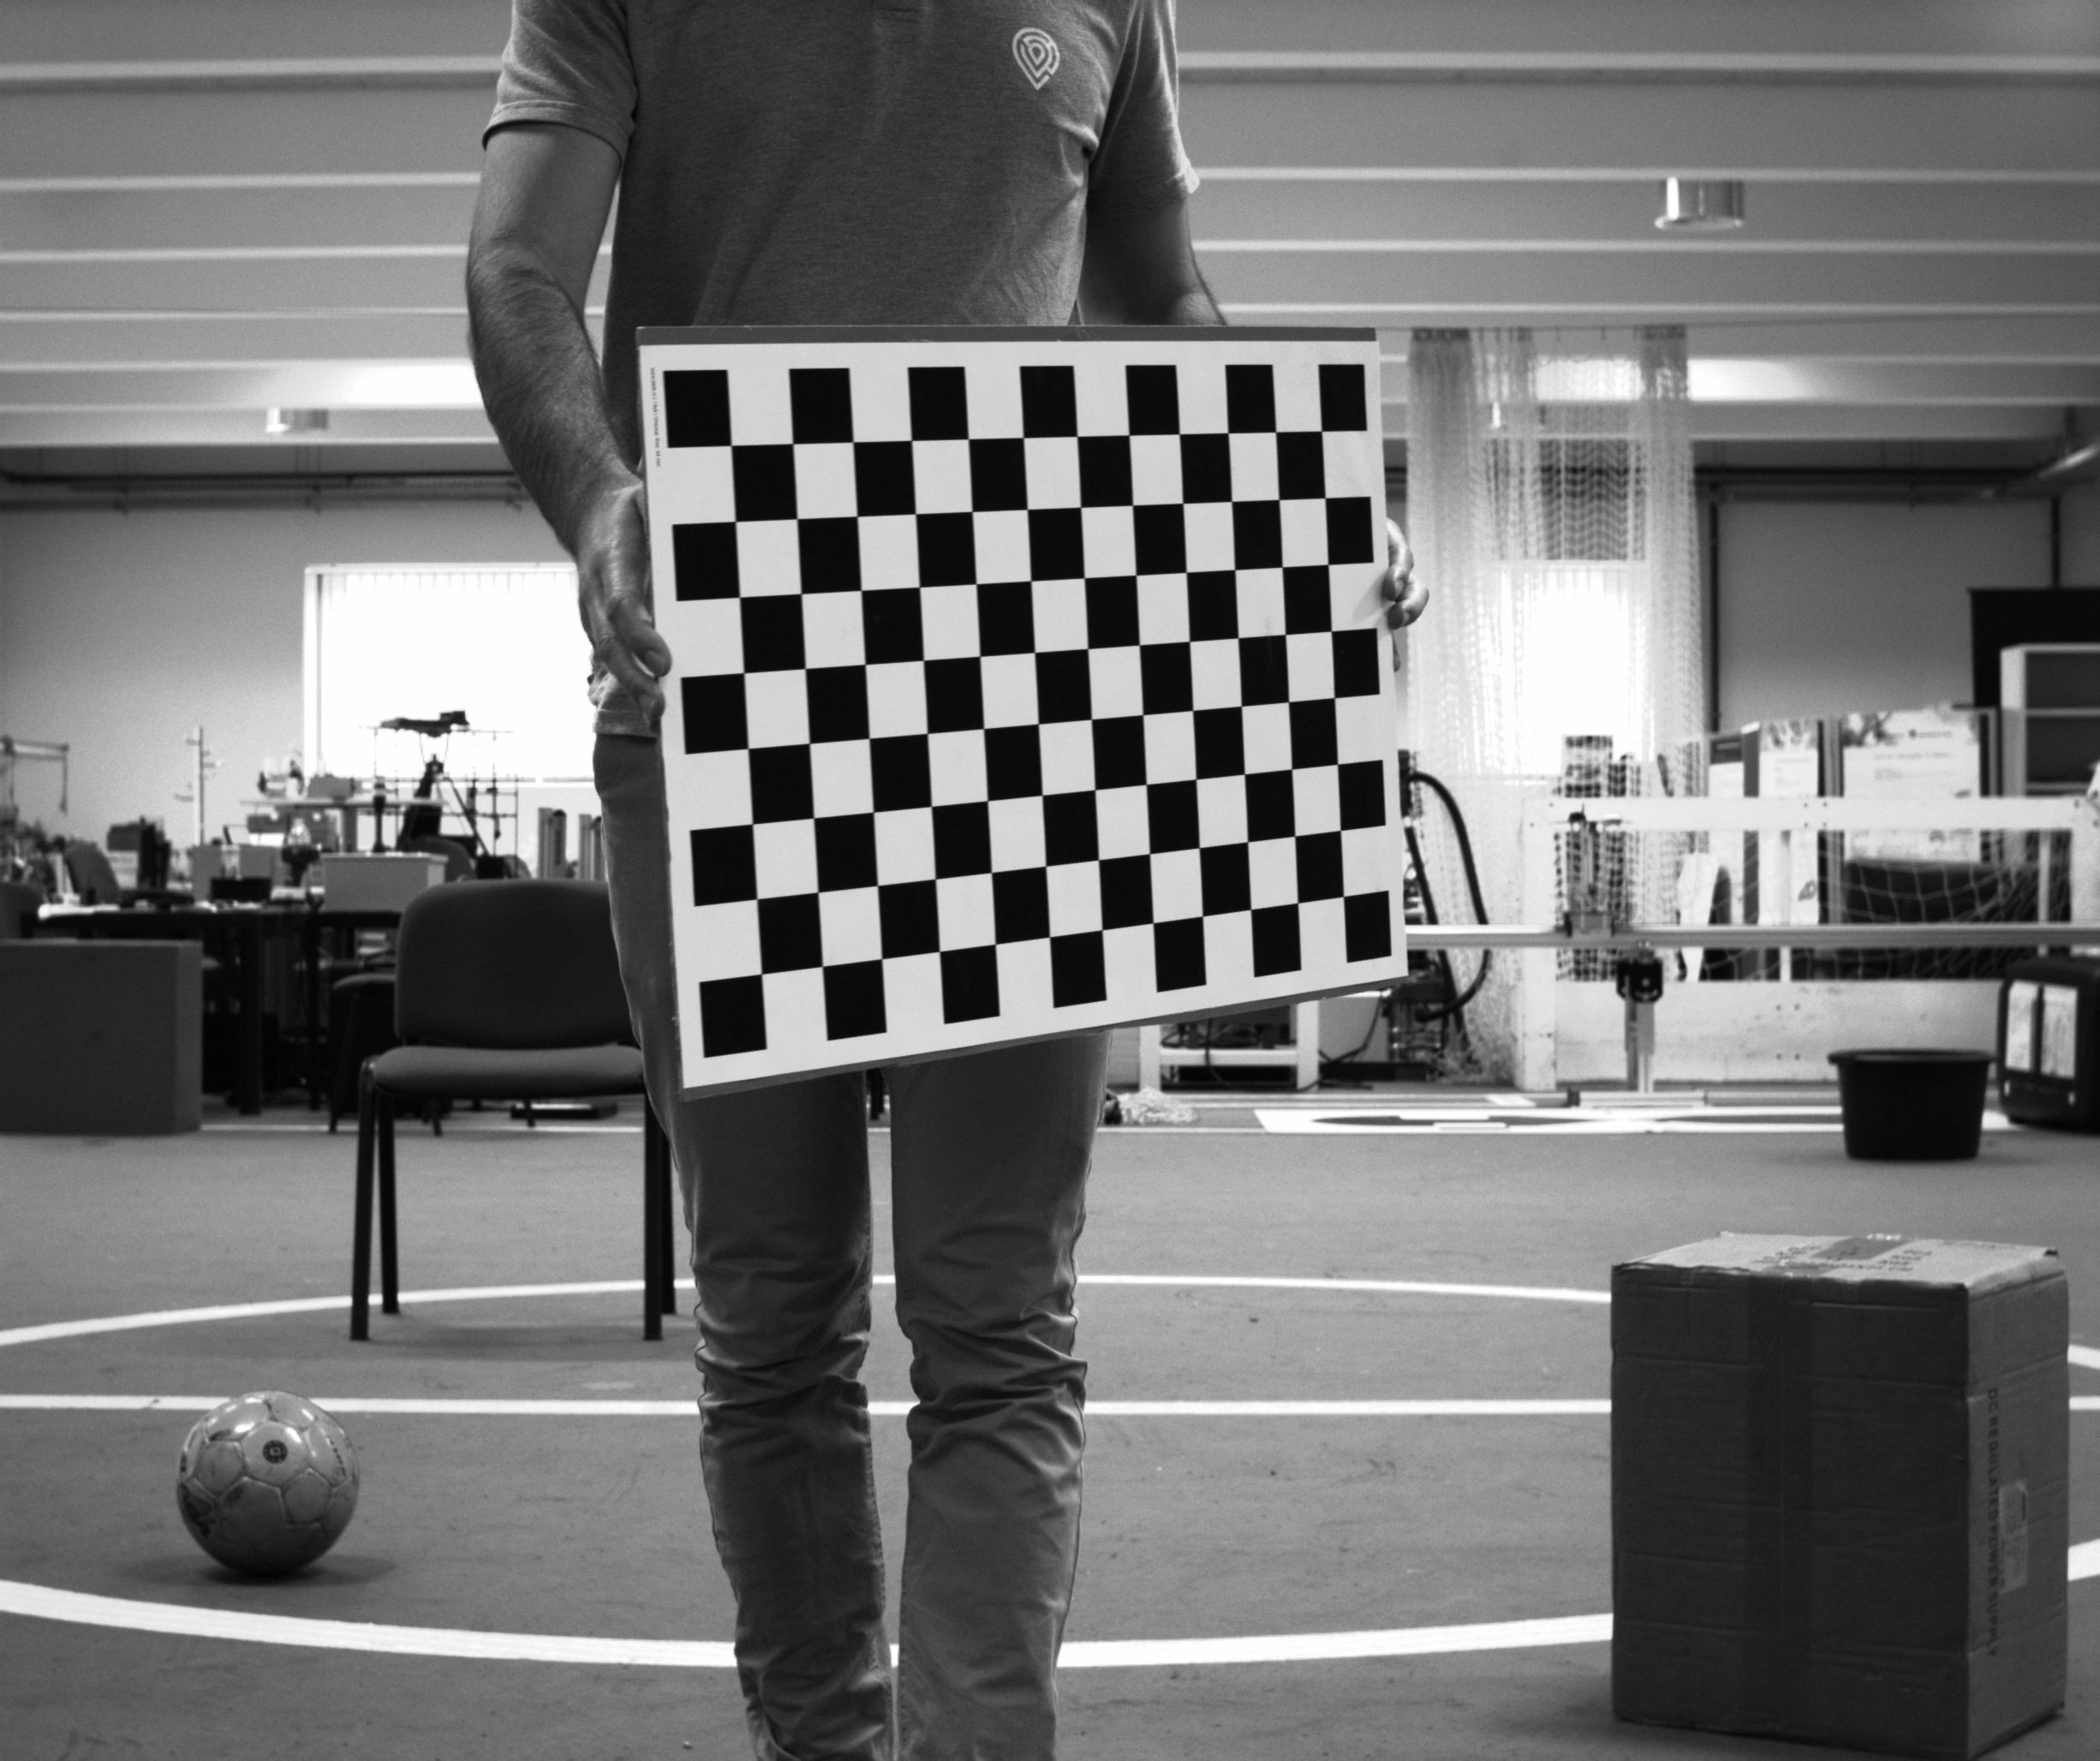
\includegraphics[width=0.9\textwidth]{img/camera-calibration/left-0005.png}
	\end{subfigure}
	\begin{subfigure}[c]{0.30\textwidth}
		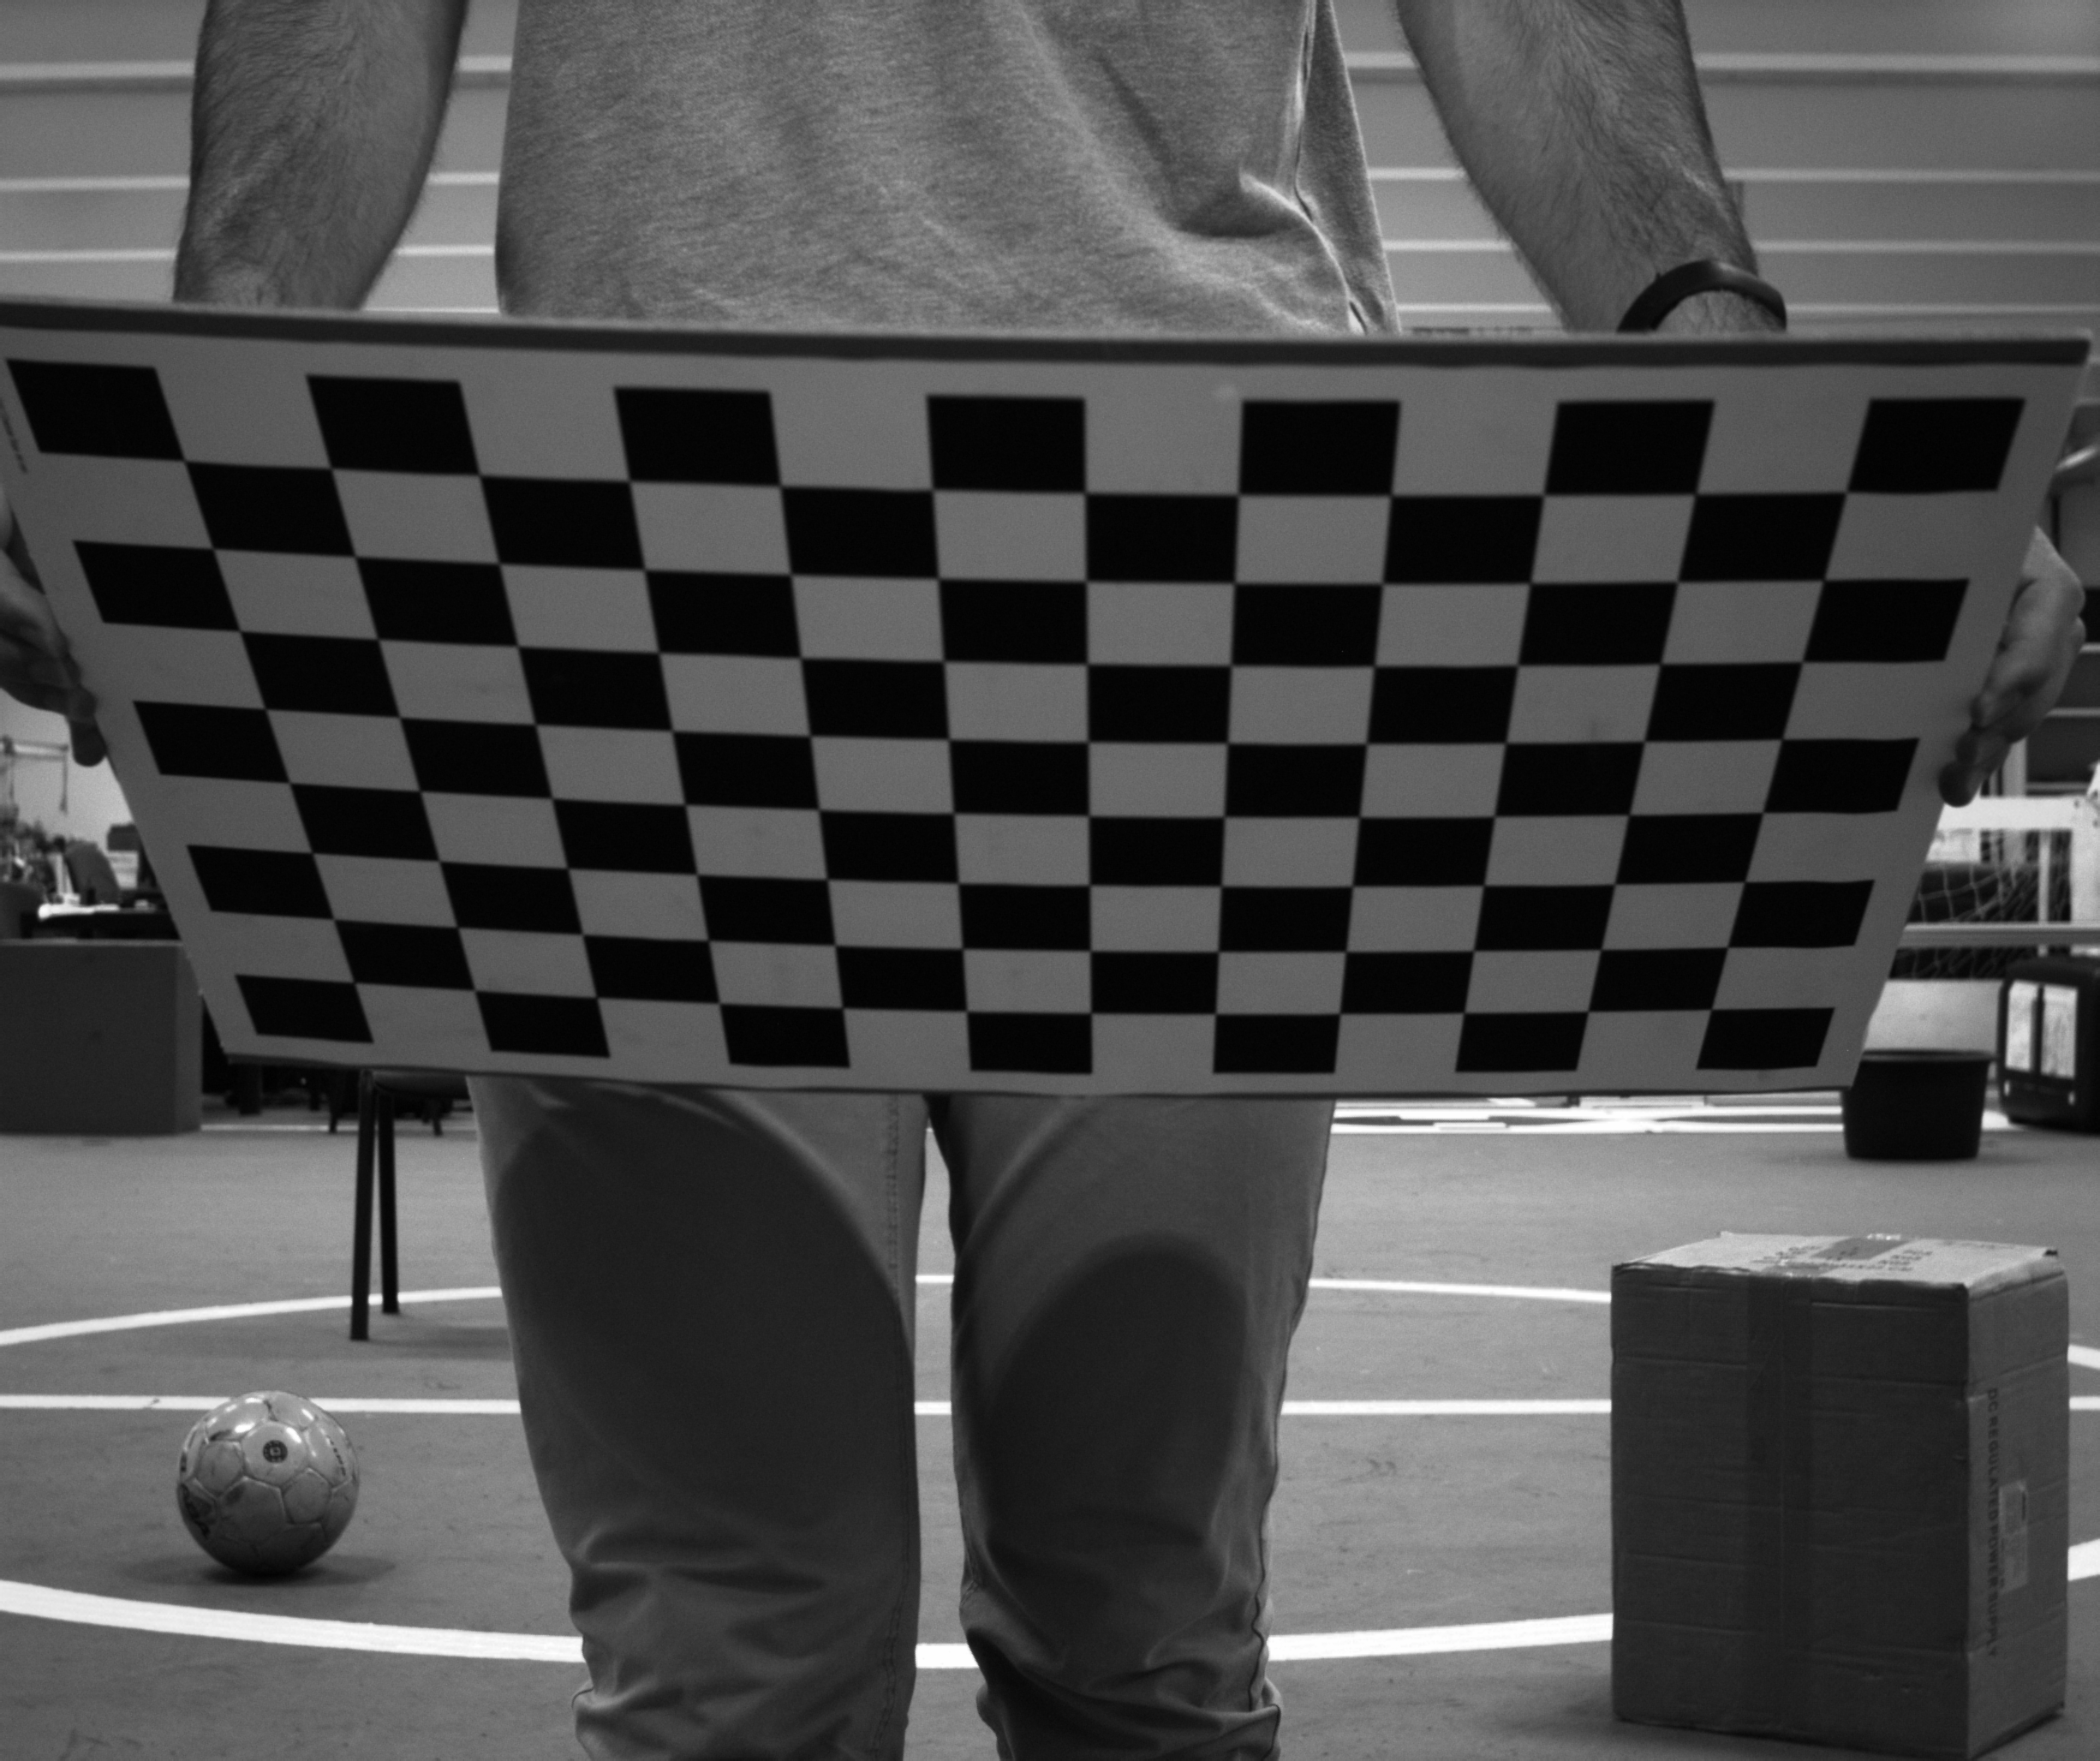
\includegraphics[width=0.9\textwidth]{img/camera-calibration/left-0022.png}
	\end{subfigure}
	\\ 
	\vspace{5mm}
	\begin{subfigure}[c]{0.30\textwidth}
		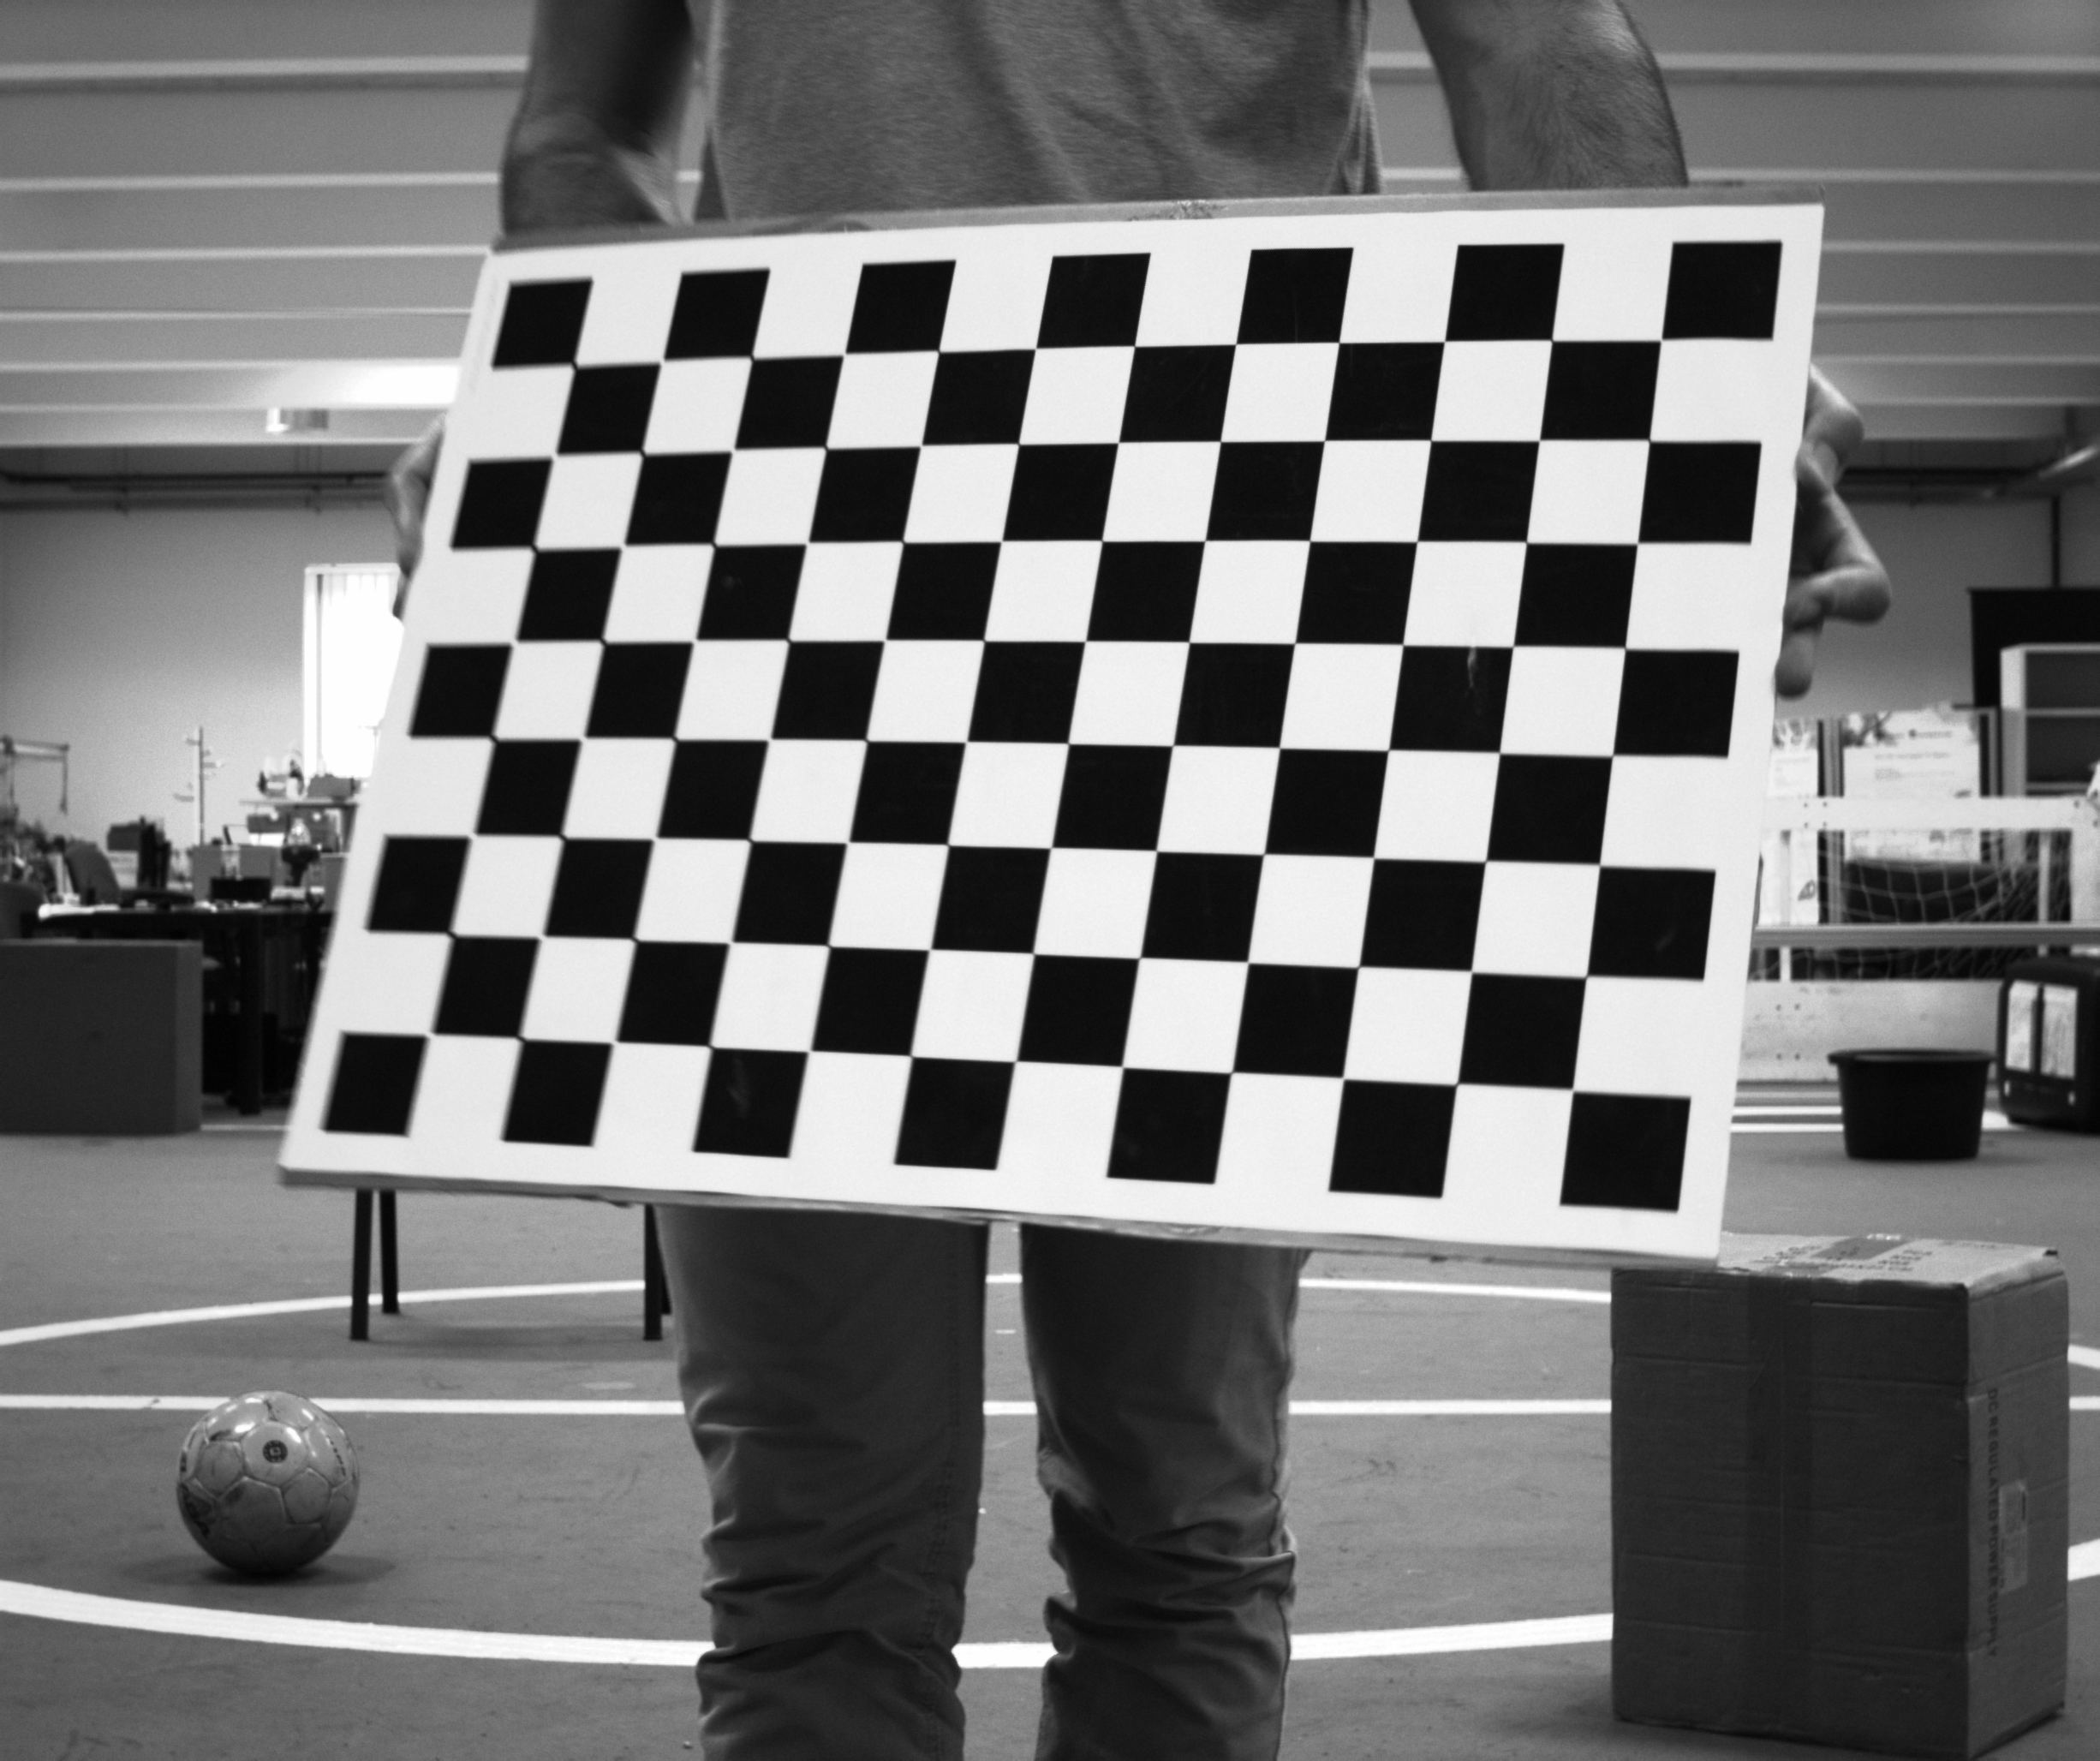
\includegraphics[width=0.9\textwidth]{img/camera-calibration/left-0030.png}
	\end{subfigure}
	\begin{subfigure}[c]{0.30\textwidth}
		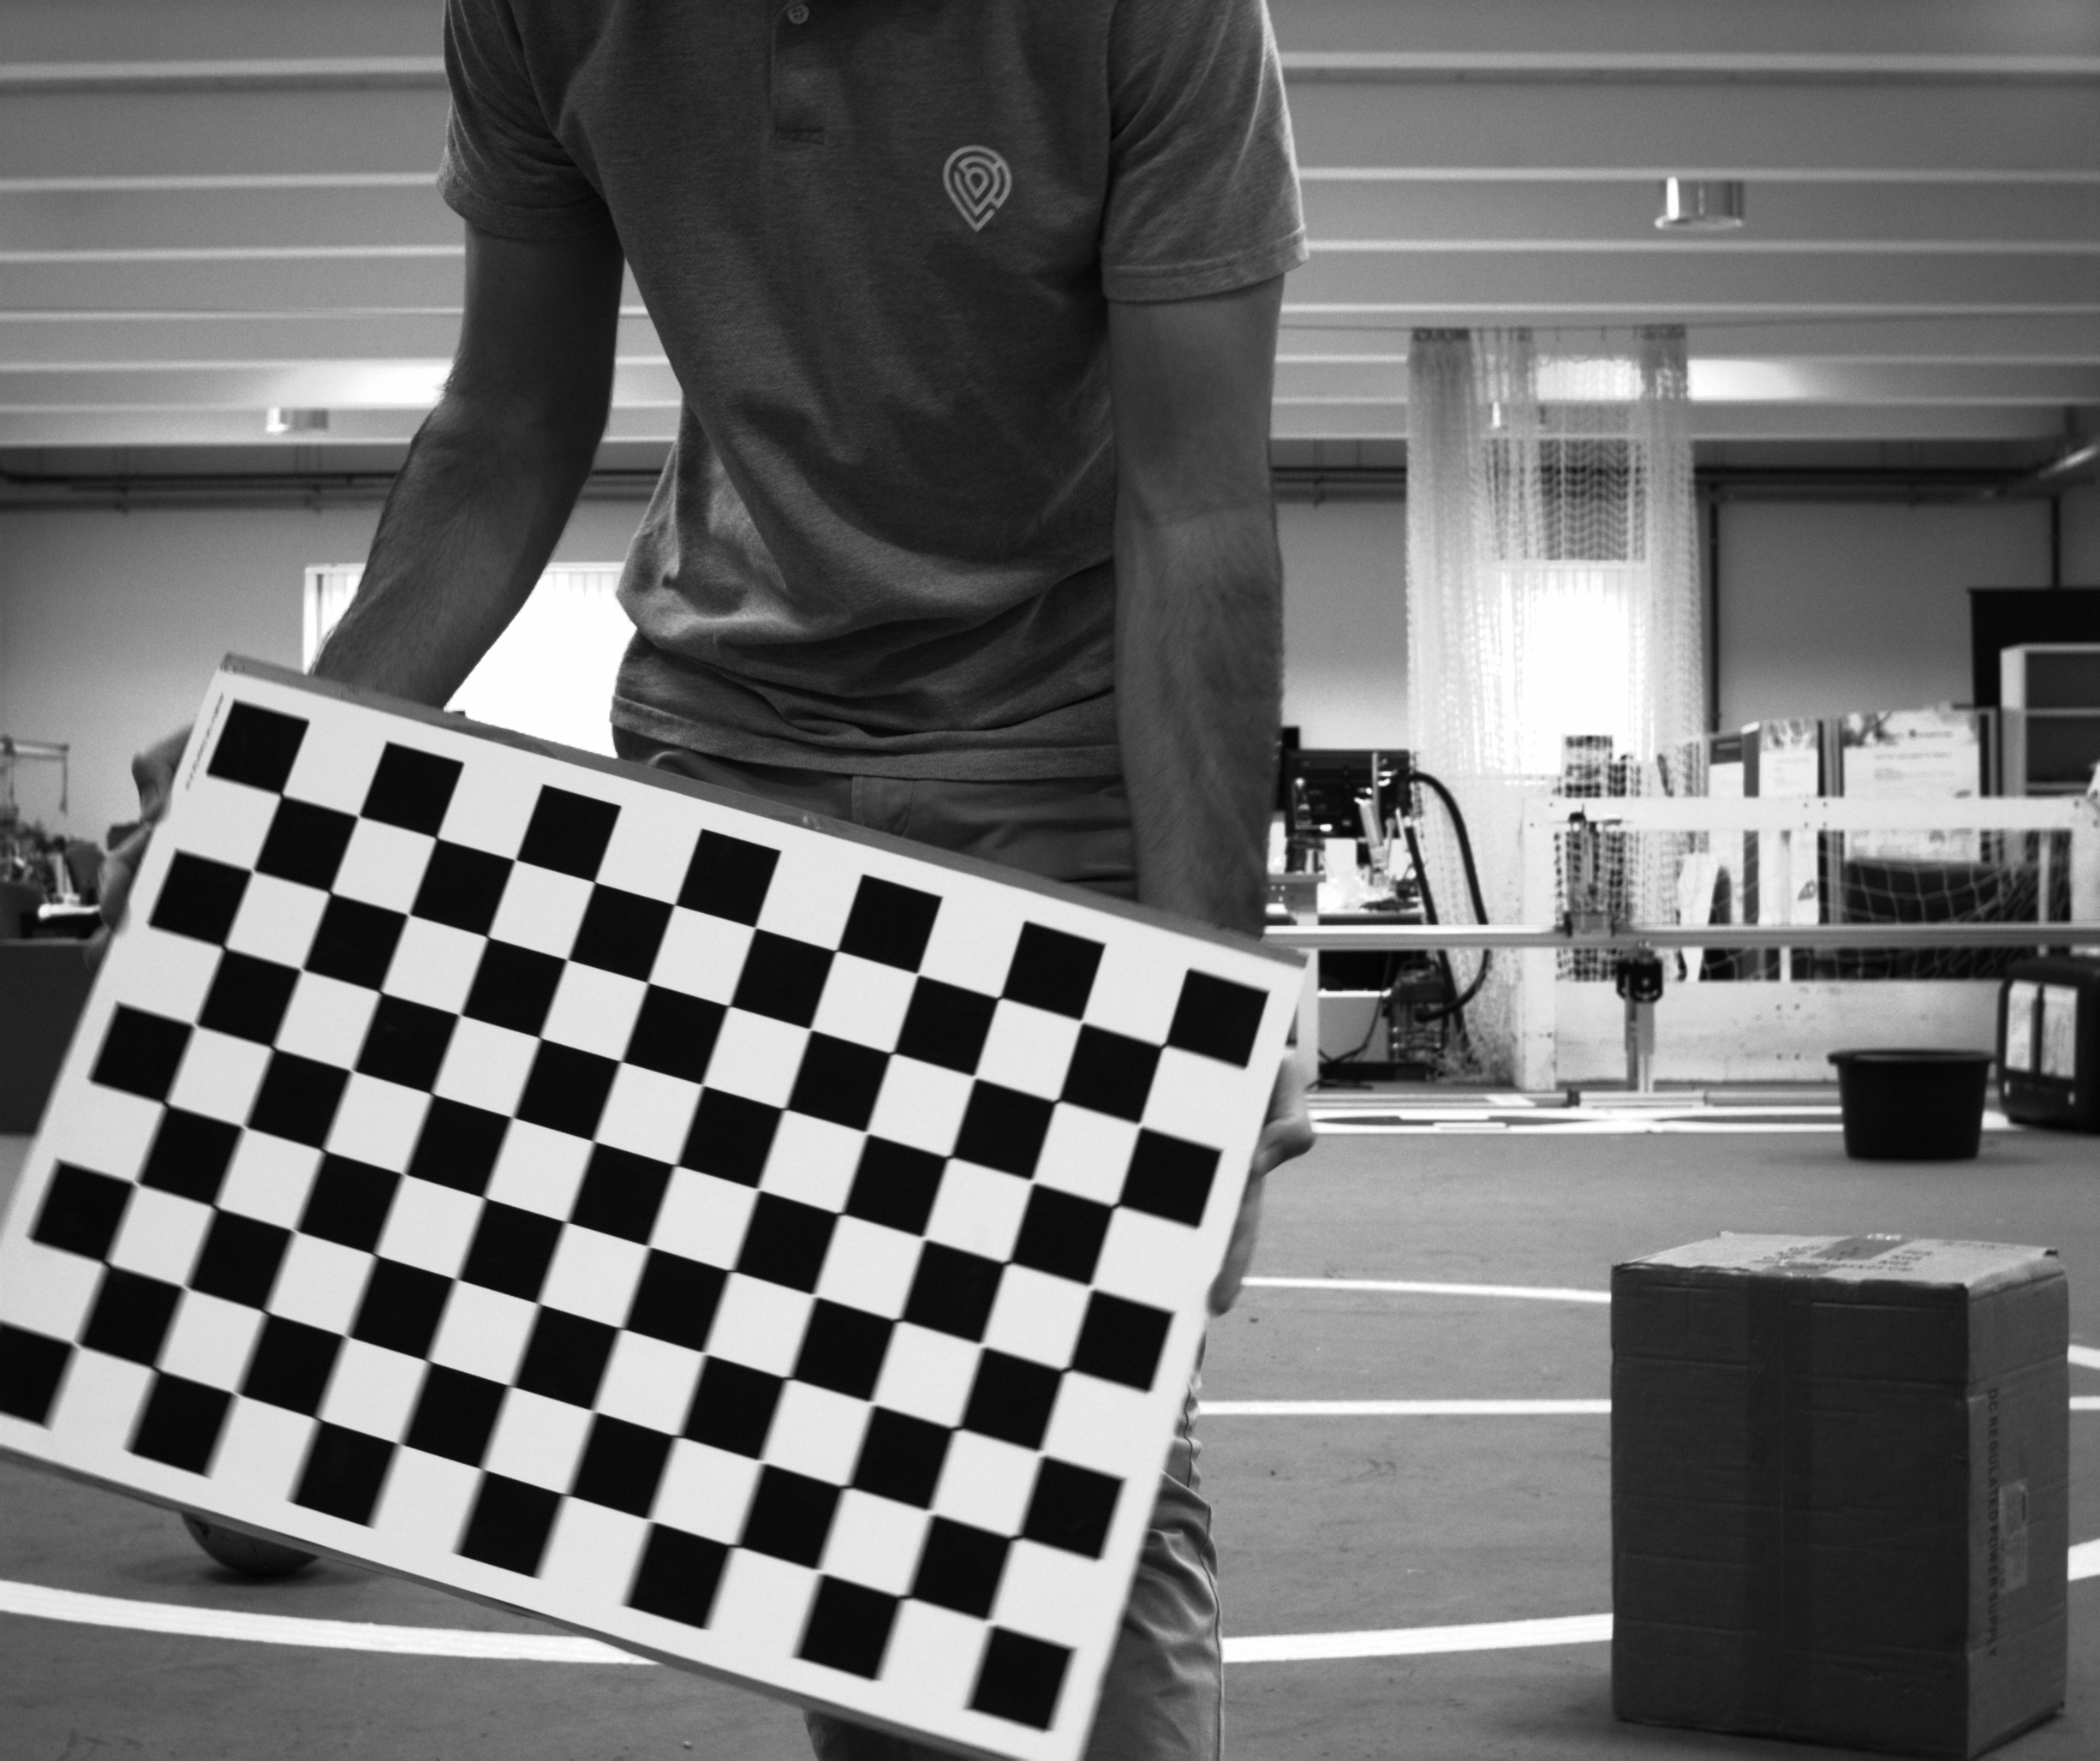
\includegraphics[width=0.9\textwidth]{img/camera-calibration/left-0044.png}
	\end{subfigure}
	\begin{subfigure}[c]{0.30\textwidth}
		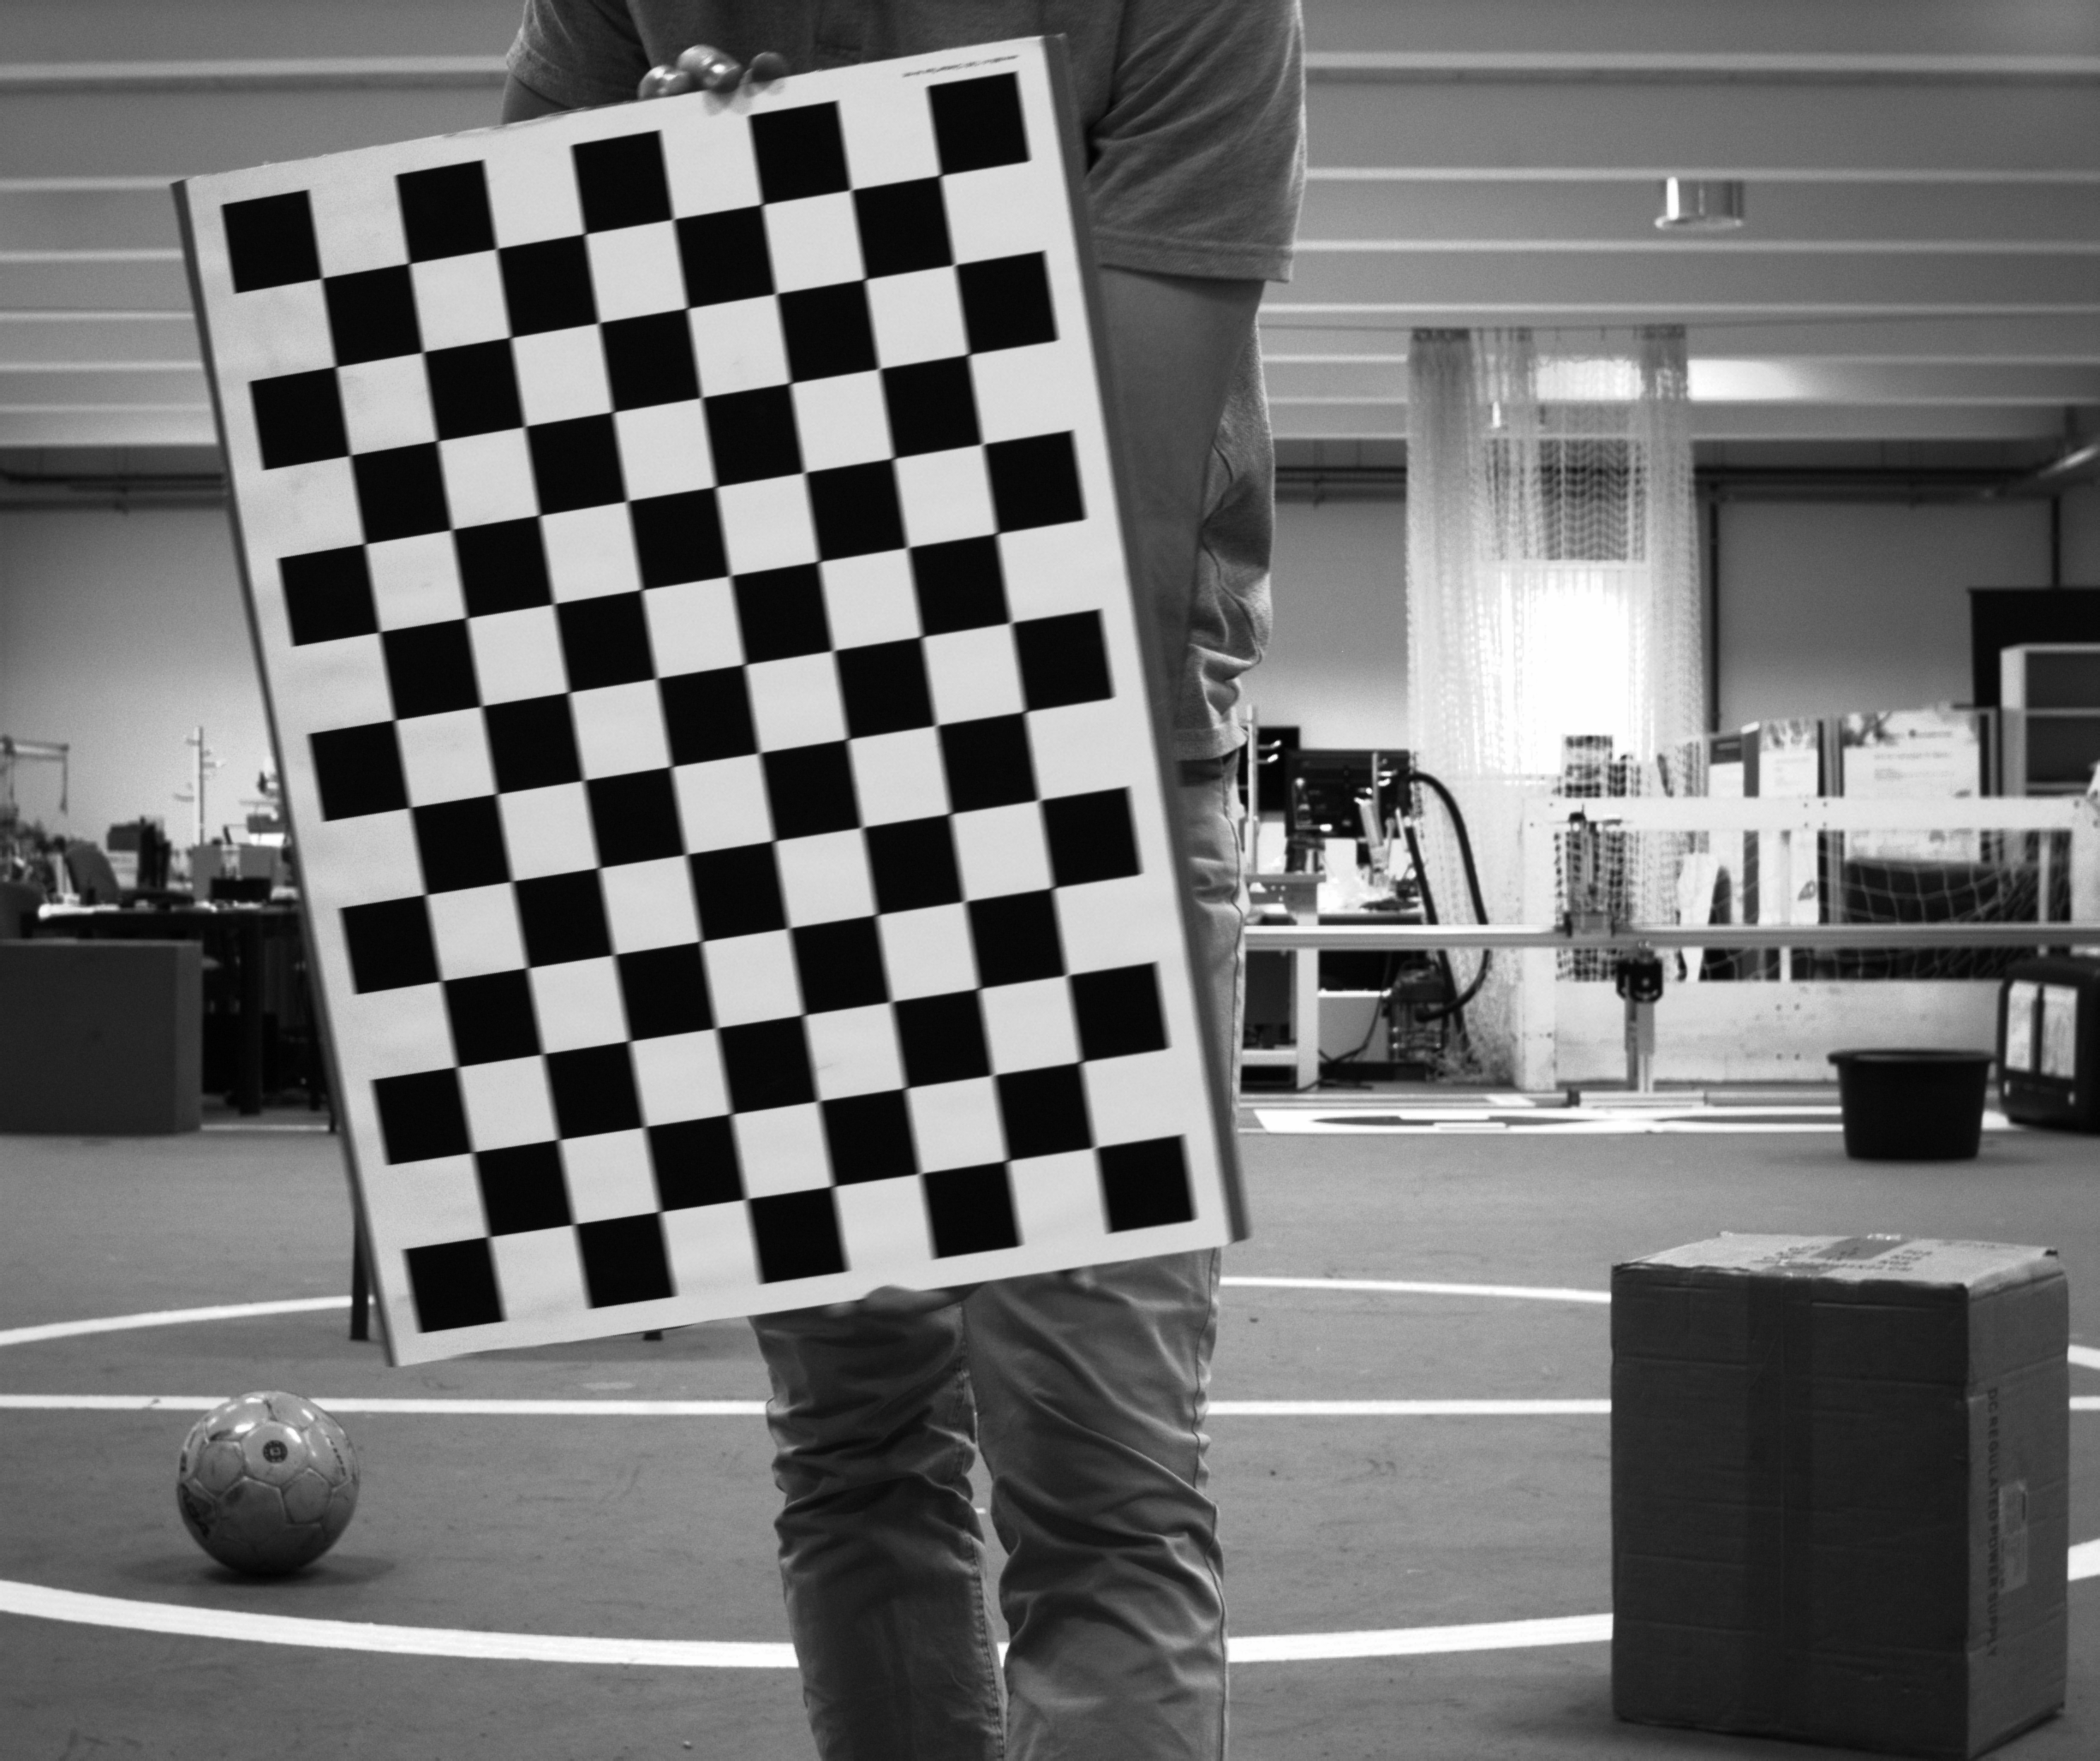
\includegraphics[width=0.9\textwidth]{img/camera-calibration/left-0048.png}
	\end{subfigure}
	
	\caption[Subset of figures used for intrinsic camera calibration.]{Subset of 6 figures used on camera intrinsic calibration. The figures are all on greyscale and for each figure, the chessboard pattern was moved to generate a unique rotational matrix and translation vector in relation to the camera coordinate frame.}
	\label{fig:camera-calibration-images}
\end{figure}

\subsubsection{Frame Rate and Bandwidth concerns}
Despite the straightforwardness of the process, one of the secondary goals of this thesis is to produce a dataset of scenarios on which \ac{lidar} interference is present. Such goal implies that all data must be properly recorded, organized and stored, including calibration data. \ac{ros} provides \texttt{rosbag}, a package for recording and playing back messages exchanged in a \ac{ros} network, which is used to save data on an external hard-drive.

However, preliminary tests with this tool indicate that it cannot save image topics at $9.2$~\ac{fps}. Other tests have shown that $8$~\ac{fps} is the best scenario where \texttt{rosbag} can record data without causing buffer flush due to overrun errors. 

When calibrating the camera, \texttt{camera\_calibration} package drops the frame rate to $\approx 4$~\ac{fps}, because it cannot operate at the desired data flow. If de-Bayerization\footnote{Converting the raw data, stored on a Bayer Filter raw format, to a RGB image} and/or rectification is being applied to the image for saving a pre-processed image, frame rate drops to $\approx 2$~\ac{fps}, since \texttt{image\_proc}, the package responsible for pre-processing the image, cannot process images at the data-rate required for them to be saved on disk, introducing an overhead. Therefore, all images are sent from camera on the raw format \texttt{BayerGB8} and recorded with \texttt{rosbag} in the same format. Note that despite the camera providing  the \texttt{RGB8Packed} color format, the hardware processing required on the camera hardware forces frame rate to be below $8$ \ac{fps}, reason why it was not chosen.

At 8~\ac{fps}, the bandwidth occupied by a 5~\ac{mp} image stream is $8 \cdot 2452 \cdot 2056 \approx \SI[per-mode=symbol]{40}{\mega\byte\per\second}$. Manta's bandwidth limit configuration register was set to a value $25\%$ higher, \SI[per-mode=symbol]{50}{\mega\byte\per\second}, to accommodate other transmissions from the computer to camera and vice-versa. No bandwidth problems were registered, besides occasionally frame drops on the starting or ending of computer processes.

Therefore, for normal operation, Manta \ac{avt} G-504C is set to trigger image capture at a fixed frame rate of $8$~\ac{fps} and when being under an internal calibration procedure, at $4$~\ac{fps}. If better computer hardware has available, internal calibration procedure could be runt at the same frame rate as normal operation, since the bottleneck is on the computer.

However, to ensure the camera runs at the desired number of \ac{fps}, other parameters that affect frame rate must also be managed, such as exposure time.


\subsubsection{Lens Aperture and Exposure Time}
Thorlabs\cp~MVL16M1 lens has several possible apertures: $f/1.4$, $f/2.0$, $f/2.8$, $f/4.0$, $f/8.0$, $f/16.0$. The smaller the F-number\footnote{F-number represents the ratio of the lens' focal length to its effective aperture diameter.}, the bigger the entrance aperture, allowing the camera sensor to be exposed to more light within the same time interval. More light indicates that exposure time can be reduced, since the sensor receives the same amount of light in less time to produce a sharp image.

However, decreasing the F-number reduces the Hyperfocal distance (see Equation~\eqref{eq:hyperfocal_distance}), which in turn reduces the \acf{dof}. A trade-off must then be addressed between \ac{dof} and F-number, which implies that three parameters must be fine-tuned: \ac{dof}, exposure time and image frame rate, since they are all interconnected. As stated above, a maximum \ac{fps} is desirable, but due to recording constraints of the \texttt{rosbag} package, $8$~\ac{fps} is the target image frame-rate. This implies that, at $8$\ac{fps}, the camera must never take more than \SI{125}{\milli\second} since the start of exposure to the broadcast of the message on the Ethernet network, which means that exposure time must be shorter. Through experimental analysis, the maximum exposure which seems to not disturb the desired frame rate is \SI{100}{\milli\second}. 

The F-number needs to be adjusted not only to ensure the requirements of the exposure time are met and to maximize \acl{dof}, but also to ensure that exposure can be increased or decrease to accommodate the daylight intensity variations. Considering a maximum exposure time of \SI{100}{\milli\second}, only aperture values greater than $f/4.0$ result on a sharp image under those constraints. To maximize the \ac{dof}, the smaller F-number should be chosen, since \ac{dof} and the F-number are inversely proportional. Therefore, with such constrains, our experimental setup uses an F-number of $f/4.0$ and an exposure time that varies between \SIrange{80}{100}{\milli\second} during daylight.

\subsubsection{\acl{dof} and calibration object}
\label{subsec:calibration:dof-and-calibration-object}
Solving Equation~\eqref{eq:hyperfocal_distance} and replacing its result on Equation~\eqref{eq:dof-subject-distance}, we can obtain $d$, the object distance at which the camera must be focused. The object to be focused is the calibrating pattern and the $DoF_{near}$ limit is select to be the distance at which the calibration pattern fills the camera~\ac{fov}. The calculations can be seen in Equation~\eqref{eq:hyperfocal-and-dof-values}.

\begin{subequations}
	\label{eq:hyperfocal-and-dof-values}
	\begin{align}
		H & = \frac{16mm^2}{4.0 \cdot 0.020mm} + 16mm  = 3.216 m \label{eq:hyperfocal-distance-value} \\
		\vspace{25mm}
		d & = \frac{(3.216 - 16mm) \cdot 1.405}{3.216 - 1.405} = 2.49m \label{eq:dof-subject-distance-value}
	\end{align}
\end{subequations}

After focusing the camera, the \texttt{cameracalibrator.py} node is run, using the command below. Note that the chessboard patterns argument is $12\times 8$ and not $13 \times 9$, because the \texttt{size} argument refers to the number of interior corners, not number of squares on the chessboard.


\begin{verbatim}
    rosrun camera_calibration cameracalibrator.py --size 12x8 --square 0.044  
        monocular:=/camera image:=/camera/image_raw
\end{verbatim}


After the \ac{gui} registers all the images, the calculation of calibration parameters can be initiated and the parameters are saved on a \textit{.ost} file for later use and/or sent the configuration to the camera. 

To interact with the Manta AVT G-504C, \texttt{avt\_vimba\_camera} \ac{ros} package~\cite{AVTROSdriver}, which depends on VIMBA GigE SDK, is used to operate the camera. It also provides compatibility with the \texttt{camera\_calibration} package, crucial for a straightforward calibration process.

\subsection{Camera Calibration Results}
The \ac{ros} node diagrams can be seen on Figure~\ref{fig:camera-calibration-rosgraph}. On sub-Figure~\ref{fig:camera-calibration-bag-rosgraph}, the nodes and topics for the calibration procedure using the data published by the \texttt{rosbag} tool. On sub-Figure~\ref{fig:camera-calibration-avt-rosgraph}, the nodes and topics for the calibration procedure using the data directly from the driver are shown. 


\begin{figure}[H]
	\vspace{5mm}
	\centering
	\begin{subfigure}[c]{0.8\textwidth}
		\centering
		\def\svgwidth{\columnwidth}
		\graphicspath{{img/camera-calibration/}}
		\includesvg{img/camera-calibration/bag-rosgraph-print}
		%
\includegraphics[width=0.8\textwidth]{img/camera-calibration/bag-rosgraph.png}
		\caption{\ac{ros} node graph for the camera calibration procedure using the \texttt{rosbag} tool. \texttt{RosbagPlayer} is the node that plays back the data stored on the bag file.}
		\label{fig:camera-calibration-bag-rosgraph}
	\end{subfigure}
	\vspace{5mm} \\ 
	\begin{subfigure}[c]{0.8\textwidth}
		\centering
		\def\svgwidth{\columnwidth}
		\graphicspath{{img/camera-calibration/}}
		\includesvg{img/camera-calibration/avt-rosgraph-print}
		%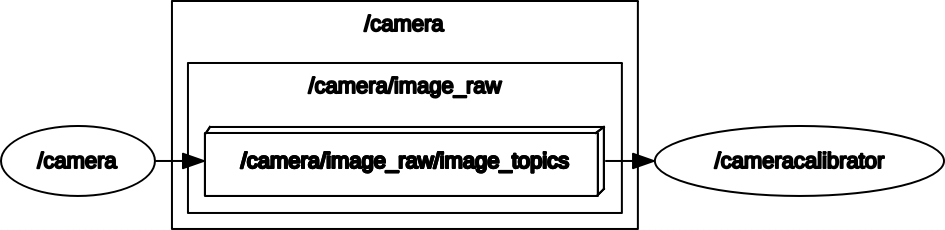
\includegraphics[width=0.8\textwidth]{img/camera-calibration/avt-rosgraph.png}		
		\caption{\ac{ros} node for the camera calibration procedure using the \ac{avt} Vimba \ac{ros} driver. \texttt{camera} node refers to \ac{ros} node that wraps the \ac{avt} Vimba driver.}
		\label{fig:camera-calibration-avt-rosgraph}
	\end{subfigure}
	\caption[Camera calibration \acs{ros} node diagram.]{Camera Calibration node graph for \ac{ros} nodes. \texttt{cameracalibrator} is the node responsible for computing the intrinsic camera calibration parameters, either if they are (\subref{fig:camera-calibration-bag-rosgraph}) being replayed using \texttt{rosbag}; (\subref{fig:camera-calibration-avt-rosgraph}) or coming directly from the camera driver.}
	\label{fig:camera-calibration-rosgraph}
\end{figure}

The camera was calibrated daily whenever experimental measures were taken. The calibration for one of these days is shown below, where $\mathbf{K}$ is the camera intrinsic parameters' matrix, $\mathbf{D}$ is the lens distortion coefficients vector and $\mathbf{P}$ the camera projective matrix. %on Equation~\eqref{eq:camera-calibration-results}.

\begin{subequations}
	\label{eq:camera-calibration-results}
	\begin{align}
		\mathbf{K} & = 
		\begin{bmatrix}
			4595.944192 & 0.0         &  1313.9194945 \\
			0.0         & 4593.466666 &  952.554450 \\
			0.0         & 0.0         &  1.0
		\end{bmatrix} \nonumber \\
		\mathbf{D} & = 
		\begin{bmatrix}
			-0.304037 & 1.364428 &  -0.005705 & 0.003330 & 0.0
		\end{bmatrix} \nonumber \\
		\mathbf{P} & = 
		\begin{bmatrix}
			4529.381836 & 0.0         & 1318.010062 & 0.0 \\
			0.0         & 4534.939941 & 947.167736  & 0.0 \\
			0.0         & 0.0         & 1.0         & 0.0 
		\end{bmatrix}
		\nonumber
	\end{align}
\end{subequations}

	

\section{\ac{lidar} Intrinsic Calibration}
\label{sec:calibration:lidar}
Unlike a camera, \acp{lidar} do not possess a typical calibration procedure. For Velodyne VLP-16 reflectivity measurements are factory calibrated, in a procedure described in~\cite{vlp16} and a \ac{xml} file is provided with the \ac{lidar}, containing corrections for the \ac{lidar} operating parameters.

This file must be converted to a more suitable format, \acs{yaml}~\footnote{\acs{yaml} is an acronym for \acl{yaml}. The author chose not to follow the norm of expanding acronyms' inline due to acronym recursive nature, to facilitate reading.}, which is \ac{ros} default and can be loaded by the Velodyne \ac{ros} driver package, \texttt{velodyne}, for correction of the \ac{lidar} measurements. After observing the point cloud with test objects such as boxes and walls, \ac{lidar} calibration is observed to be accurate and no further calibration procedures were undertaken.

\section{Camera and \ac{lidar} Extrinsic Calibration}
\label{sec:calibration:extrinsic}
Calibrating the camera and \ac{lidar}, as explained in Section~\ref{subsec:sota:camera-intrinisc-calibration}, requires determining the rigid body transform between the reference frames of the two sensors. A rigid body transform, also known as a Euclidean Isometry since it preserves the distance between points~\cite{mvg_book}, has 6 degrees of freedom, that can be represented by a translation and a rotation vector.

Due to the ambiguity of the rotation vector and its variety of interpretations: (1) it can represent one of twelve Euler angles notation, angle axis notation, amongst others; (2) this notation is normally replaced by the unambiguous rotation matrix (see Equation~\eqref{eq:camera_transform_full} for an example) or a quaternion. Such representations are also free from gimbal lock, a mathematical limitation of the vector representation, that can cause one rotation axis ``locking'' on another, resulting on their rotation no longer being independent of the other, removing one degree of freedom and degenerating into a two-dimensional rotational space. For more details on gimbal lock and other singularities see~\cite{mvg_book, Slabaugh, camera_models}.

In this thesis, the preferred notation is a quaternion, which is also adopted by \ac{ros}~\cite{Foote2014}. A quaternion is a mathematical object belonging to $\mathbb{R}^4$, that has a vector (or imaginary) part and a scalar (or real) part. Its representation is denoted on Equation~\eqref{eq:quaternion-notation}, where $\mathbf{i}$, $\mathbf{j}$ and $\mathbf{k}$ are the normalized unit vectors of the $x$, $y$ and $z$ axis, respectively; and $w$ is the scalar part. More information on quaternions can be found on~\cite{mvg_book}.

\begin{equation}
	\label{eq:quaternion-notation}
	q = (x\mathbf{i}, y\mathbf{j}, z\mathbf{k}, w)
\end{equation}

\subsection{Calibration Method}
\label{subsec:calibration:calibration-method}
Given the nature of the sensors: a camera image is two-dimensional and the \ac{lidar} data is tridimensional; the extrinsic calibration needs to consider the projective geometry and its transformations on the camera. Revisiting Equation~\eqref{eq:jointRotationTranslationTransform}, our goal is to determine the joint rotation and translation matrix that allows the conversion of coordinates from the \ac{lidar} to the camera frame. To account for projective geometry, Equation~\eqref{eq:camera_transform_full} must be considered when establishing 3D points to image pixels correspondences.

The method implemented to calibrate the camera and \ac{lidar} is inspired by Scaramuzza's\etal~\cite{Scaramuzza} and Brabec's~\cite{brabec2014} work. The method proposed consists on manually selecting the correspondences between image pixels and 3D points on the \ac{lidar} point cloud. If a single synchronized frame from the camera and \ac{lidar} is used, one can consider the scene as static, and therefore, the joint rotation and translation matrix present in Equation~\eqref{eq:camera_transform_full} is actually the same as the matrix present on Equation~\eqref{eq:jointRotationTranslationTransform}. 

Such considerations are only possible due to the camera using a global shutter instead of rolling shutter. In the former, the image is acquired in a single shot and all the points ``have the same timestamps''. In the latter, each row of the image is acquired one after another, iteratively, therefore, ``having different timestamps''. If a rolling shutter camera was used, for a single image, the \ac{lidar} point cloud could not have been considered static and the delays on the camera shutter and \ac{lidar} rotation would have to be taken into account when calibrating and fusing the data between the two. An exception to the latter is if the \ac{lidar} and camera position is static and the scene is also static.

Since the intrinsic calibration matrix is already obtained by the method described on Section~\ref{sec:calibration:camera}, and the correspondences are selected by the user, the only remaining unknown is the joint rotation and translation matrix. Also, since this method ``reuses'' the equations that are the basis for intrinsic camera calibration, it can also ``reuse'', with some constraints and modifications, the same algorithms~\cite{opencv_doc}, such as \texttt{solvePnP}, which determines the joint rotation and translation matrix that converts world points to camera pixels.


\subsection{Implementation}
To extrinsically calibrate the camera and \ac{lidar}, a multi-node network approach was followed, which can be seen on Figure~\ref{fig:extrinsic-calibration-rosgraph}, on Appendix~\ref{appendix:appendix-diagrams}. Using \ac{opencv} and \ac{pcl}, two visualizers were encapsulated under \ac{ros} nodes written in C++, that subscribe camera and \ac{lidar} messages, respectively. The point cloud visualizer, \texttt{PCL\_Viewer\_with\_Pose}, receives the point cloud data from the \texttt{rosbag} player or the \texttt{velodyne} driver and publishes the coordinates of the selected point and the viewer pose. \texttt{Image\_Visualizer} publishes the pixels selected by the user, but requires the de-Bayering and conversion to RGB of the raw image using the \texttt{image\_proc} package. Despite being wrapped in \ac{ros}, each of the visualizers provides standalone callbacks, that support ``frame freezing'' for correspondences selection.

Another node, \texttt{rigid\_transform\_computation} is responsible for listening to messages containing the selected pixels and points, registering their correspondences. This node  instantiates two \ac{ros} services servers, that can be called asynchronously: one for computing the rigid body transform and another to save the correspondences selected on a \ac{csv} file, for later usage. 

%\begin{figure}[!ht]
%	\centering
%	\def\svgwidth{\columnwidth}
%	\graphicspath{{img/calibration/}}
%	\includesvg{img/calibration/extrinsic-calibration-rosgraph-print}
%	\caption{\ac{ros} node graph for the extrinsic calibration. The nodes are represented in  ellipses and the topics between them in rectangles. Rosbag Player is responsible reproducing the recorded topics.}
%	\label{fig:extrinsic-calibration-rosgraph}
%\end{figure}


The algorithm implemented to compute the 6 degrees of freedom rigid body transformation uses \ac{opencv} \texttt{solvePnP}, which gives the intrinsic camera parameters and the manually selected correspondences between the object points (3D points from \ac{lidar}). It can also compute the rotation and translation vectors. For solving the \ac{pnp} problem, several algorithms can be used: Levenberg-Marquardt~\cite{Levenberg1943}, Effective~\ac{pnp}~\cite{Lepetit2009}, Perspective-Three-Point~\cite{Gao2003}, Direct-Least-Squares~\cite{Hesch2011} or Exhaustive Linearization — Uncalibrated \ac{pnp}~\cite{Penate-Sanchez2013a}. The \ac{ros} node implemented provides an argument to select the desired algorithm to be applied to solve the \ac{pnp} problem.

After resolving the \ac{pnp} with one of the methods above, Rodrigues' algorithm is used to convert the \ac{opencv} rotation vector to a rotation matrix~\cite{Dai2015}, which is then used to derive the quaternion. Combining the quaternion with the translation vector, a static transform is published to the \ac{ros} network, which can be used to convert and fuse data from the camera coordinate frame to the \ac{lidar} and vice-versa.

An additional \ac{ros} node is also created to compute and publish the rigid body transformation from pre-selected correspondences. It loads the correspondences between the 3D points and image pixels from the \ac{csv} file, the camera intrinsic parameters from an \acs{yaml} file. Using the same algorithms as \texttt{rigid\_transform\_computation}, it computes the rigid body transform and publishes it to the \ac{ros} network using \ac{ros} static transformation.


\subsection{Calibration Result}
\label{subsec:calibration:extrinsic-results}
To ease the calibration process, a \ac{ros} launch file is created. A launch file is written in \ac{xml} and provides instructions to \ac{ros} master node on how to run all the necessary nodes to implement a desired functionality. On this case, \texttt{rigid\_transform\_computation.launch}, launches the two visualizers (image and point cloud) and the node responsible for listening to the selected correspondences. 

Several tests were performed with the possible algorithms for solving \ac{pnp}. Since for the version of \ac{opencv} used, $3.2.0$, the Direct-Least-Squares and Uncalibrated \ac{pnp} methods are unstable~\cite{opencv_doc}, with only the Levenberg-Marquardt, Perspective-Three-Point and Effective~\ac{pnp} were tested. 

Although the planar chessboard used for intrinsic camera calibration was present during the extrinsic calibration, the algorithm implemented does not require the usage of a calibration object. For calibration, 6 points were selected in the point cloud and 6 pixels on the image: four of them correspond to the corners of the chessboard and two to a background object. The selected correspondences can be seen in Figure~\ref{fig:calibration-correspondences}: sub Figure~(\subref{fig:extrinsic-calibration-correspondences:camera}) shows the selected pixels on the image, marked with red crosses; sub Figure~(\subref{fig:extrinsic-calibration-correspondences:lidar}) shows the selected 3D points on the point cloud, marked as red spheres.


\begin{figure}[H]
	\centering
	\begin{subfigure}[c]{0.39\textwidth}
		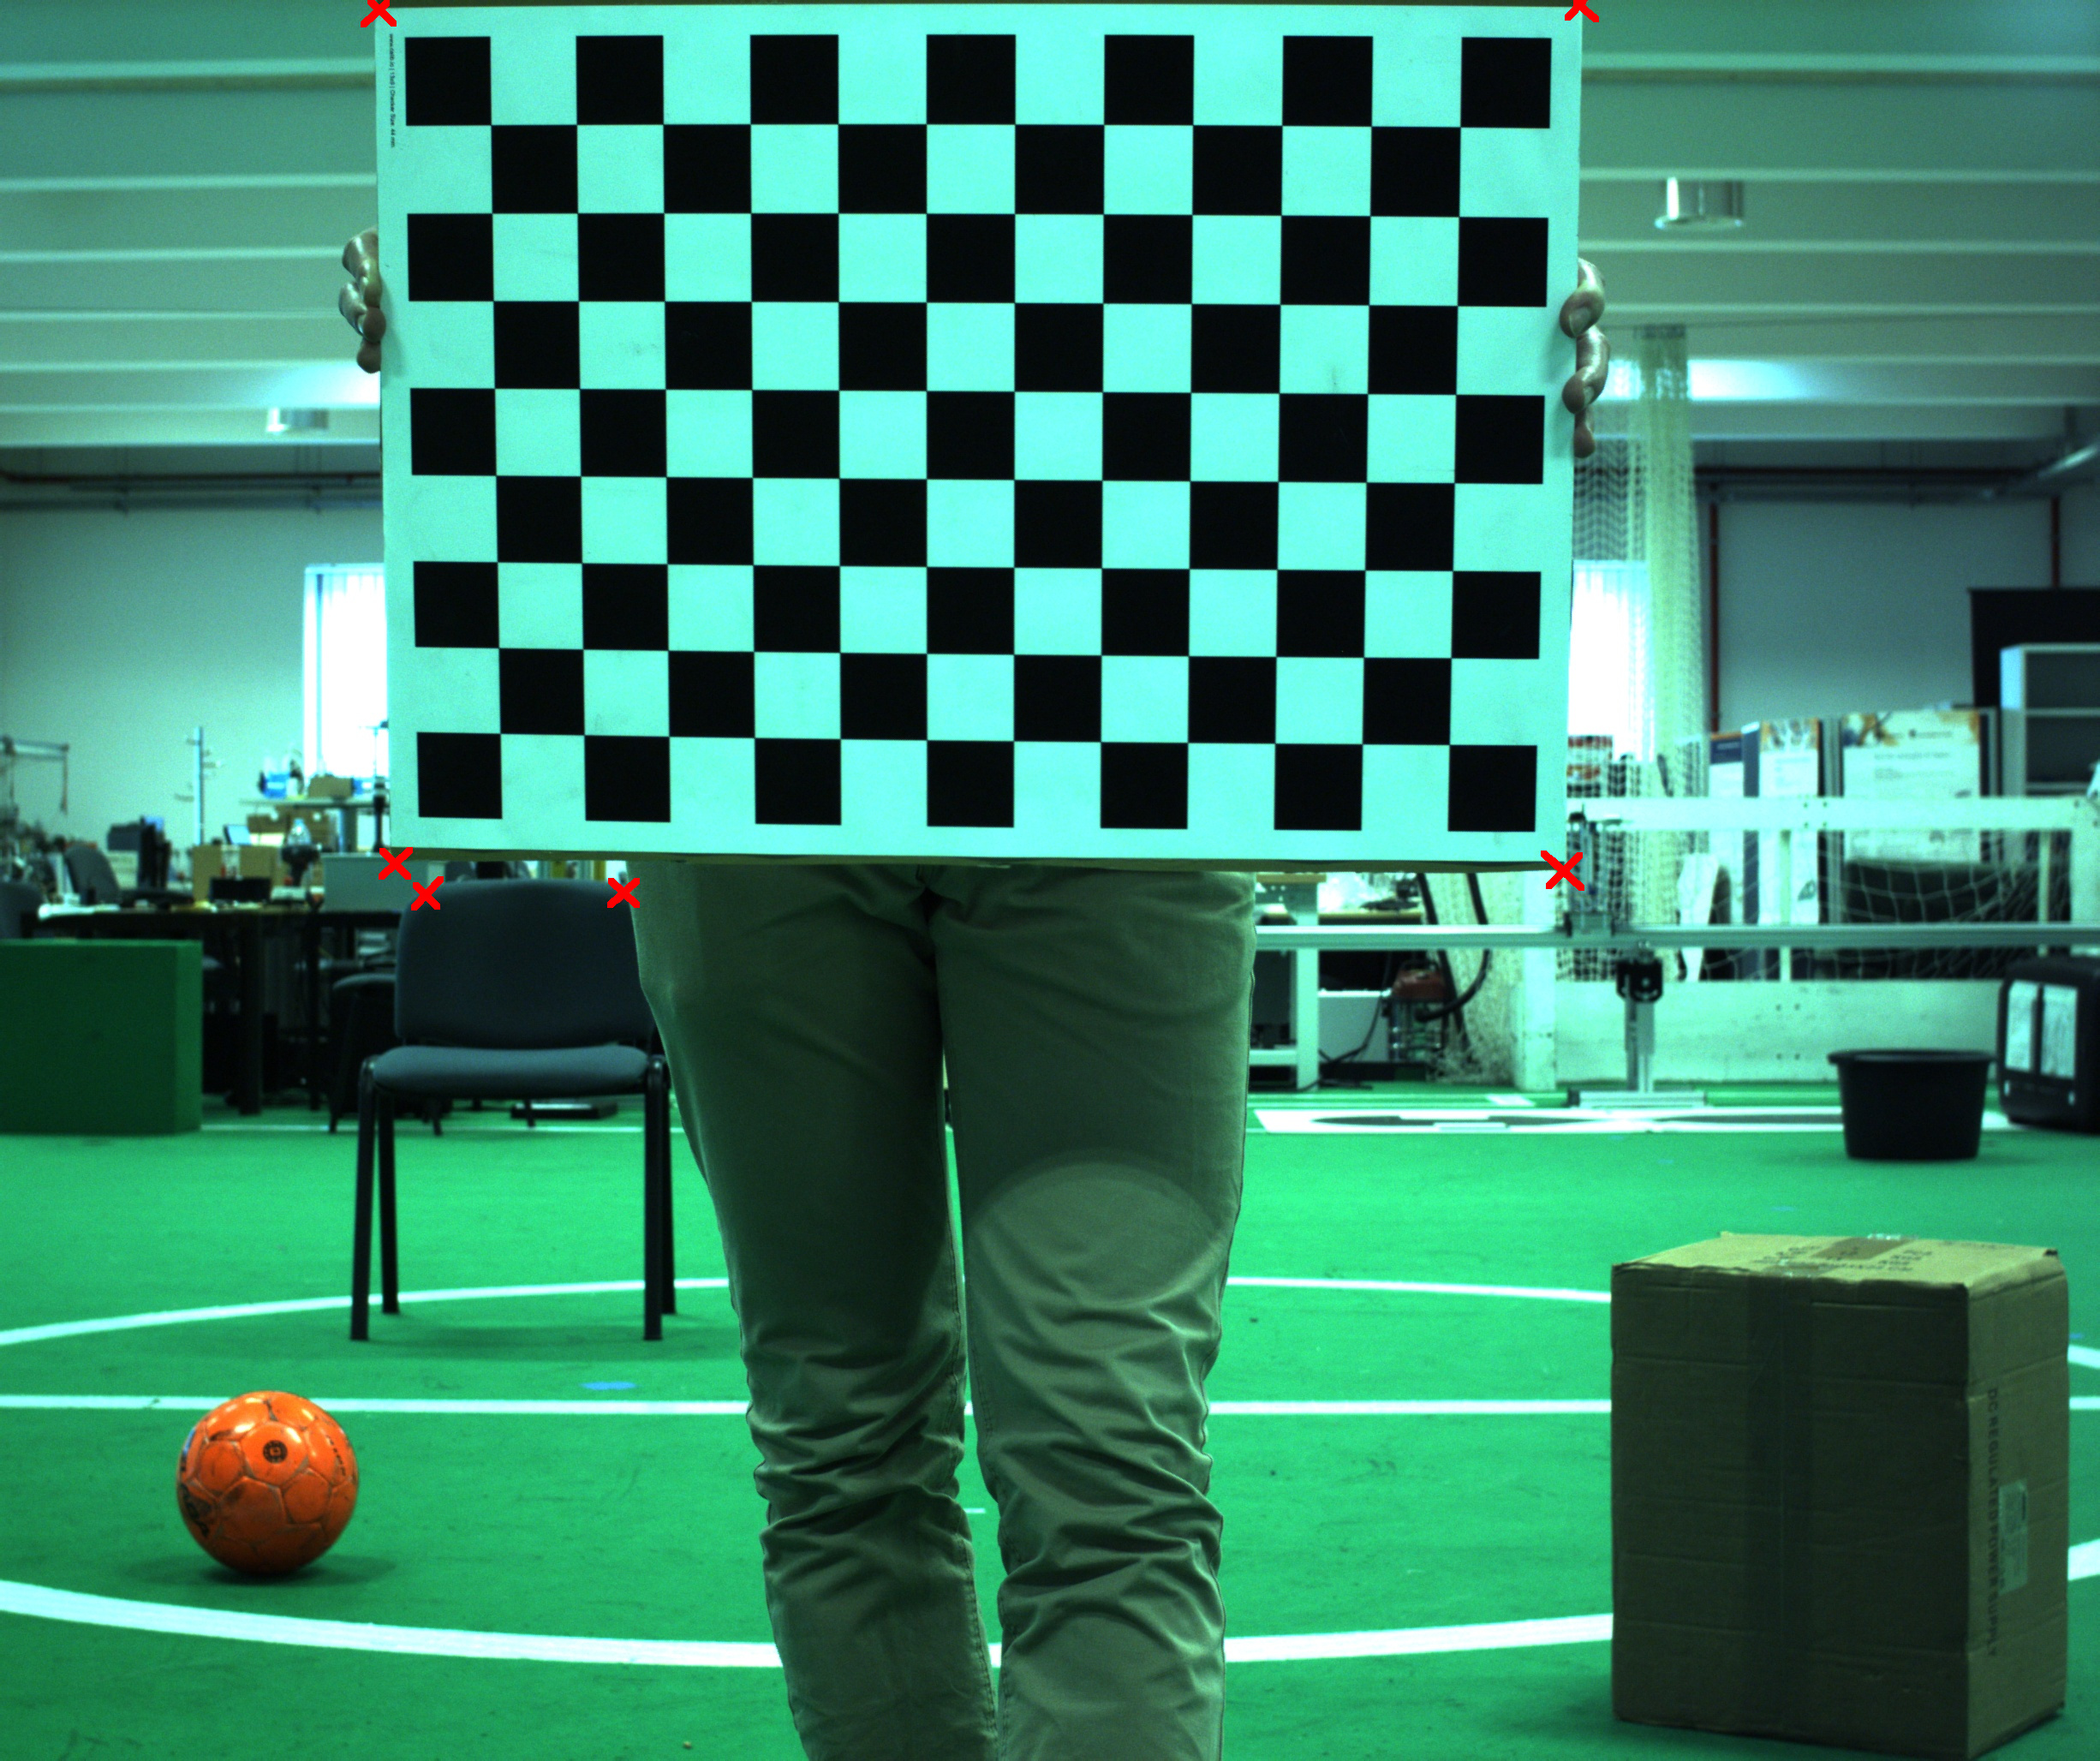
\includegraphics[width=\textwidth]{img/calibration/camera-extrinsic-calibration-points-draw.jpg}
		\caption{}
		\label{fig:extrinsic-calibration-correspondences:camera}
	\end{subfigure}
	\qquad
	\begin{subfigure}[c]{0.55\textwidth}
		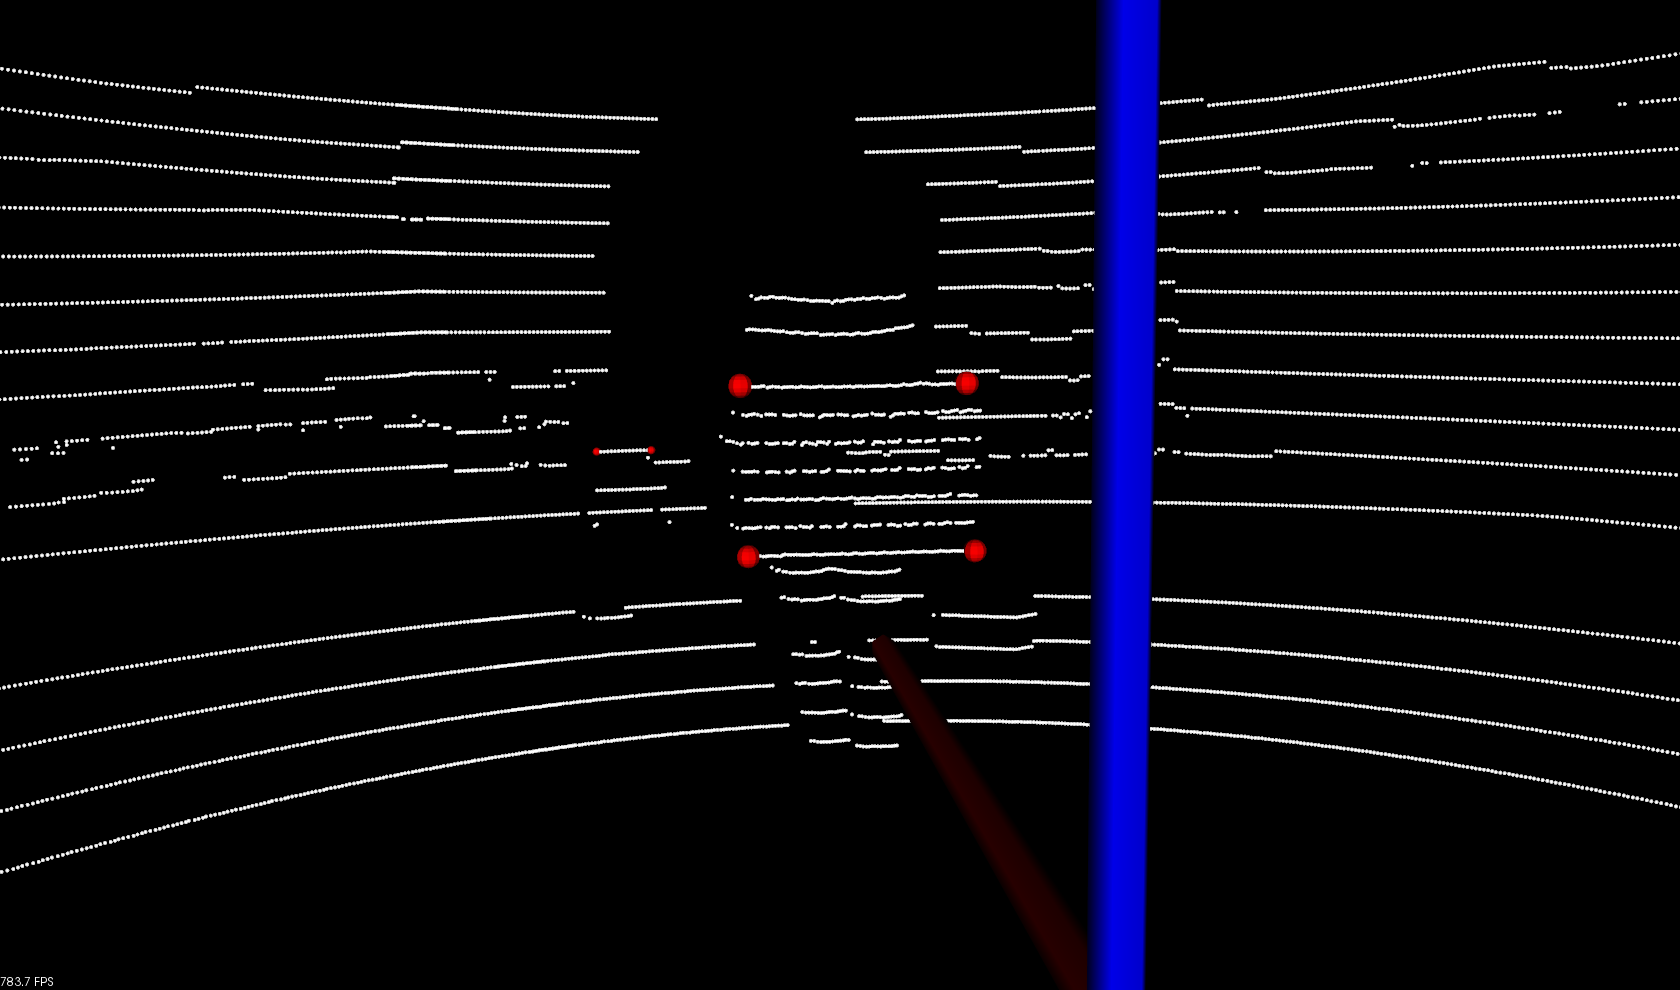
\includegraphics[width=\textwidth]{img/calibration/lidar-extrinsic-calibration-points.png}
		\caption{}
		\label{fig:extrinsic-calibration-correspondences:lidar}
	\end{subfigure}
	\caption[Correspondences selected on the image and point cloud for extrinsic calibration between the two.]{Image~(\subref{fig:extrinsic-calibration-correspondences:camera}) and Region of the Point Cloud~(\subref{fig:extrinsic-calibration-correspondences:lidar}) used on the extrinsically calibration between the camera and the \ac{lidar}. The correspondences are marked with red crosses or spheres, respectively, and correspond to the 4 corners of the chessboard and the limit of the chair on the background.}
	\label{fig:calibration-correspondences}
\end{figure}

After the manual selection of the points, the rotation and translation are obtained from the camera frame to the \ac{lidar} frame. If the transformation from the \ac{lidar} to the camera frame is required, the inverse transformation can be obtained by inverting the scalar component of the quaternion, $w$, as depicted in Equation~\eqref{eq:quaternion-inversion}. 

\begin{equation}
	\label{eq:quaternion-inversion}
	w^\text{LiDAR}_\text{camera} = - w^\text{camera}_\text{LiDAR}
\end{equation}

Extrinsic camera and \ac{lidar} calibration was performed whenever experimental measures were taken. The calibration for the camera intrinsic parameters given on Equation~\eqref{eq:camera-calibration-results} and the correspondences shown on Figure~\ref{fig:calibration-correspondences} are presented on below. On Figure~\ref{fig:extrinsic-calibration-frames}, a visualization of the experimental setup sensors coordinate frames and the transformation between them is given.

\begin{subequations}
	\label{eq:camera-to-lidar-transform}
	\begin{align}
		t = \begin{bmatrix}
			-0.156714088124  \\
			-0.0206731034739 \\
			-0.258170823407
		\end{bmatrix} \nonumber
		& \qquad
		q = \begin{bmatrix} 
		 0.4872192 \\
		-0.4999094 \\
		 0.5216904 \\
		-0.4904560
	\end{bmatrix} \nonumber
	\end{align}
\end{subequations}

\begin{figure}[H]
	\centering
	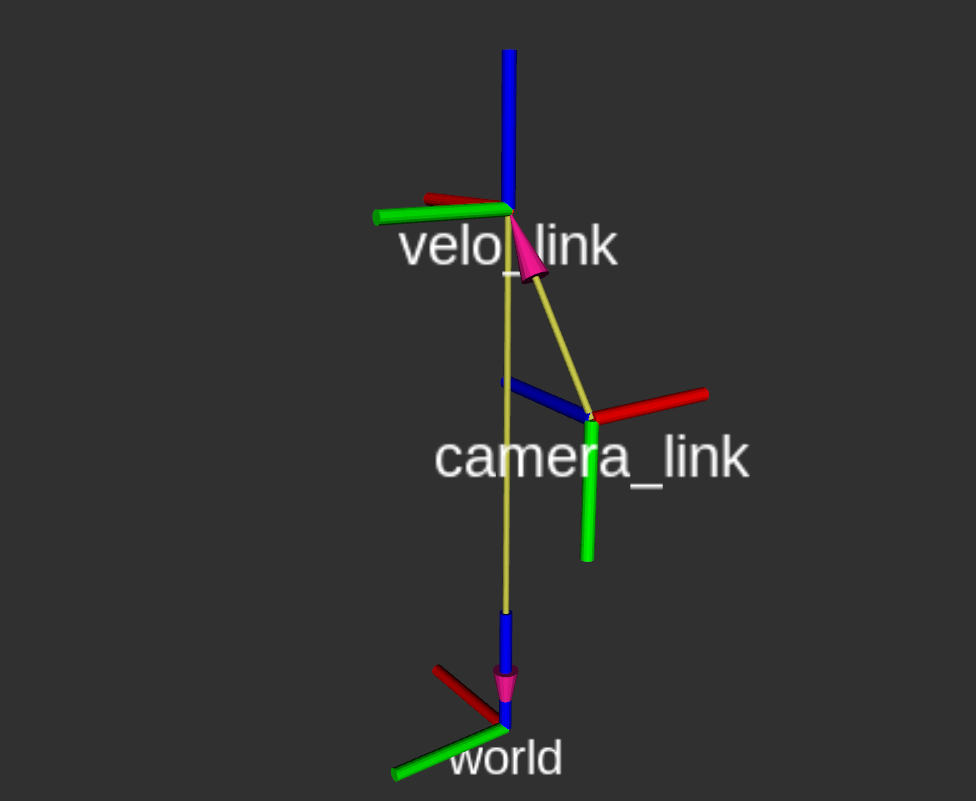
\includegraphics[width=0.5\textwidth]{img/calibration/extrinsic-calibration-frames.png}
	\caption[Experimental setup TF tree coordinate frames.]{TF visualization on \texttt{Rviz} of the TF tree between the experimental setup coordinate frames. \texttt{velo\_link} and \texttt{camera\_link} represent the coordinate frames of the Velodyne VLP-16 \ac{lidar} and the Manta \ac{avt} G-504C, respectively. The \texttt{world} coordinate frame represents the positioning of the \ac{lidar} in the world, which in this case is an offset to the vertical positioning of the \ac{lidar}.}
	\label{fig:extrinsic-calibration-frames}
\end{figure}

\subsection{Comparison with \ac{kitti}}
\label{subsec:calibration:kitti-comparison}

On \ac{kitti}, the number of coordinate frames is greater and have more complex interactions. While on the experimental setup the coordinates frames are all fixed, on \ac{kitti}, there is only one fixed frame, \texttt{world}. The car coordinate frame is named \texttt{base\_link} and the transformation between the \texttt{base\_link} and the camera are time-dependent.

On the car, every sensor has a coordinate frame, that is referred to the \texttt{base\_link} referential. From all the coordinate frames, that can be seen on~\cite{Geiger2013a}, the required during this research are:

\begin{itemize}
	\item \texttt{velo\_link}: Velodyne HDL-64E \ac{lidar} coordinate frame;
	\item \texttt{camera\_color\_left}: coordinate frame of the RGB camera selected for this research;
	\item \texttt{imu\_link}: \ac{imu} coordinate frame;
	\item \texttt{base\_link}: car coordinate frame.
\end{itemize}

Comparing with our experimental setup, the \ac{lidar} coordinate frame is equal in name and the coordinate axis orientation. The camera frame only differs in their name (the coordinate axis orientation is similar). Our experimental setup do not contain an \ac{imu}, therefore there is no need for a \texttt{imu\_link}. 

Due to the experimental setup being static, the \ac{lidar} and its \texttt{velo\_link} coordinate frame is referred directly to the \texttt{world} frame with a static transforms. Since the setup does not move, there is no need for a \texttt{base\_link} frame, since it will always coincide with the world frame, because the scene is static. On Figure~\ref{fig:kitti-tf-frames}, a subset of \ac{kitti}'s coordinate frames is presented. The \texttt{world} coordinate frame is not visible on the figure. 

\begin{figure}[!ht]
	\centering
	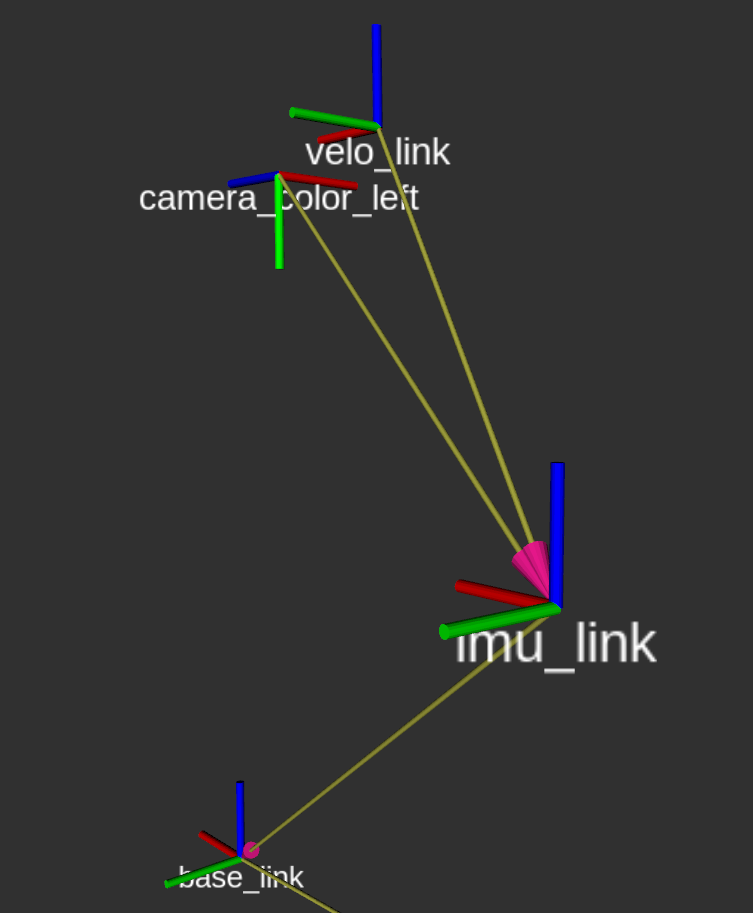
\includegraphics[width=0.5\textwidth]{img/KITTI/tf.png}
	\caption[Relevant \acs{kitti} TF tree coordinate frames.]{TF visualization on \texttt{Rviz} of the TF tree between a subset of \ac{kitti}'s setup coordinate frames. \texttt{velo\_link} and \texttt{camera\_color\_left} represent the coordinate frames of the Velodyne HDL-64E \ac{lidar} and the RGB left camera, respectively.}
	\label{fig:kitti-tf-frames}
\end{figure}

\section{Final Remarks}
\label{sec:calibration:final-remarks}

On this chapter, the experimental setup is presented and the intrinsic and extrinsic calibration of its sensors is detailed. Camera, \ac{lidar} and lens specifications are given and briefly discussed, along with their relative positioning, network setup and connection with the computer. Since camera will be used to understand and possibly mitigate \ac{lidar} interference through sensor fusion, we confirm that the camera is free from interference by the \ac{lidar} in a test without any other light sources.

Sensory calibration is performed to allow data acquisition from the camera and \ac{lidar} to construct the experimental setup dataset. Intrinsic camera calibration is carried by using \ac{ros} \texttt{camera\_calibrator.py} package and moving a chessboard in front of the camera, combining rotation and translation motions. Using Effective \acl{pnp}, the camera intrinsic matrix and the distortion coefficients for the lens are determined, which are used to rectify the camera image. Regarding \ac{lidar} calibration, the device comes calibrated by the manufacturer and only azimuthal and polar angle coefficients need to be loaded by the firmware and driver for measurement correction.

Extrinsic calibration between the camera and \ac{lidar} is performed to the determinate the rigid body transformation between the two, allowing the conversion of data between their coordinate frames. Our proposed algorithm is based on the selection of at least four $2D \leftrightarrow 3D$ correspondences between the image and the point cloud. A calibration pattern is not required. We adapt the work of Scaramuzza\etal and Brabec's, which is used to calibrate a camera, to determine the rigid body transform between the \ac{lidar} and camera, by solving for the joint rotation and translation matrix. To do so, our implementation consists of an image and point cloud visualizers, a node to receive the selected points and compute the rigid body transform and a client node to trigger the computation and saving of results.

From this chapter, our main takeout is a generic extrinsic calibration algorithm and its implementation on \ac{ros}, that can calibrated any \ac{ros} compatible monocular camera and 3D \ac{lidar}. We also intrinsically calibrate the camera, performing the first step of any computer vision project and obtain the rigid body transform between the sensors of our setup, to be used later. The work developed on this chapter is essential for the data fusion between the camera and \ac{lidar} (Chapter~\ref{chapter:sensor-fusion}) and object detection on image and estimating the correspondent bounding boxes on the point cloud (Chapter~\ref{chapter:object-detection}).

%\chapter{\acs{lidar} and Camera Data Fusion}
\label{chapter:sensor-fusion}

Data fusion consists of combining the information from two or more sources of data, that can be of equal or different types, adding value to the data set and allowing newer insights that are not possible from the parts alone, such as a representation on which is possible to understand the depth differences  between objects that are colored for easier identification. Data fusion (and sensor fusion) are two widely topics used on several areas, such as Industry 4.0, robotics and autonomous vehicles; but on the context of this research, it means that the depth information from the \ac{lidar} is combined with the color data from the camera.

A pre-requisite to combine multiple sources of data is that the rigid body transformation between the sensors is known, which allows the conversion between \ac{lidar} and camera coordinate frames. Such rigid body transform is already obtained in the previous chapter, in Section~\ref{sec:calibration:extrinsic}. Examples of sensor fusion are also been presented in Figure~\ref{fig:point_cloud_camera_fusion_example} from Section~\ref{sec:sota:sensor-fusion}.

As detailed in Section~\ref{sec:sota:sensor-fusion}, two ways are possible for combining \ac{lidar} and camera data: presenting depth information overlaid on an image or color information on a point cloud. For the purpose of this work, we are only interested on the latter, as it provides, on our opinion, a better way to verify the correctness of the calibration of Chapter~\ref{chapter:calibration} and a more interesting \ac{lidar} interference analysis and possible mitigation.

\section{Combining \acs{lidar} and Camera Data}
``Point Cloud Coloring'' consists of augmenting the information contained on a point cloud by adding to each point a RGB triplet indicating the point's color. Velodyne point clouds, besides the Euclidean coordinates of the point, also contain the intensity measurement and the laser ID/ring number\footnote{Laser ID and ring number are two concepts that can be inter-changed without loss of context. The former is more commonly used on written text while the latter is used on the source code.} of the laser and photodetector pair.

To add color data to the point cloud, two approaches can be used, depending on the source and target coordinate system:

\begin{enumerate} 
	\item \textbf{Camera $\rightarrow$ \ac{lidar}:} the camera is the source coordinate system and \ac{lidar} is the target coordinate system. The camera data is converted from the 2D image  matrix index to the \ac{lidar} 3D coordinate frame;
	\item \textbf{\ac{lidar} $\rightarrow$ Camera:} the \ac{lidar} is the source coordinate system and the camera is the target coordinate system. \ac{lidar} data is converted from the 3D \ac{lidar} coordinate frame to the camera's.
\end{enumerate}

Both approaches have their advantages and drawbacks, which will be discussed on the next two sub-sections.

\subsection{Camera $\rightarrow$ \acs{lidar}} 
Using the camera as the source coordinate system implies that the 2D pixel's information must be converted to a tridimensional format. However, when applying Equation~\eqref{eq:camera_transform_full}, depth and scale information are lost, and without further constraints, it is not possible to determine the position of the 3D point that gave origin to the image pixel\footnote{For more information, the reader is advised to research on Single View Geometry or see Part I of~\cite{mvg_book}.}. 

Therefore, re-projecting pixels to a 3D coordinate system is an under-determined system of equations, causing the geometric representation of the system to be either a ray or a quadrangular pyramid, depending on the camera sensor being considered continuous or discrete, respectively. For simplification, from now on it is considered that the 3D representation of a pixel is a ray that contains the focal point and the pixel to be projected.

After computing the ray coefficients, for data fusion the pixels projected into rays must be matched to the point cloud points. Due to the sparse nature of the \ac{lidar} data, most of the pixels do not have a correspondence with 3D points, and a criterion to reduce the number of pixels projected could be used. For the Velodyne VLP-16, the azimuthal step is \SI{0.2}{\degree} and the polar step \SI{2}{\degree}. Therefore, the number of pixels to be projected can be reduced, but that reduction must be accompanied by a solution for dealing with multiple matches and point color from multiple pixels. Dealing with multiple matches implies proposing an algorithm that decides  how to color a group of 3D points that are the correspondence of a group of pixels, since a group of pixels contains pixels with different RGB values.

Once the pixels have been projected to rays on the camera coordinate frame, before they can be matched with the \ac{lidar} points, the coefficients that define the ray must be converted to the \ac{lidar} coordinate frame.

The major drawback of this method is that for high definition images, the considerations on reducing the number of projected pixels must be taken, since the number of rays to be computed can become impractical. For our experimental setup, not considering any optimizations, would require the computation of more than 5 million rays, their projection to the point cloud coordinate frame and matching with the point cloud points.


\subsection{\acs{lidar} $\rightarrow$ Camera}
\label{subsec:sensor-fusion-lidar-to-camera}
Projecting \ac{lidar} data to the image can be performed by re-purposing Equation~\eqref{eq:camera_transform_full}: the object points are considered to be \ac{lidar} 3D point coordinates and the joint rotation and translation matrix are replaced by the rigid body transformation between the \ac{lidar} and the camera coordinate frame, which can be obtained by inverting the rigid body transformation determined in Section~\ref{sec:calibration:extrinsic}. As detailed in sub-Section~\ref{subsec:calibration:extrinsic-results}, this inversion, since we are using a quaternion notation, is equivalent to change the quaternion scalar component to its symmetric number, as depicted in Equation~\eqref{eq:quaternion-inversion}.

Projecting \ac{lidar} data to the camera coordinate frame results on a 2D point that can be used to index the image pixel matrix. However, since the \ac{lidar} \ac{fov} is wider than the camera's, it is necessary to verify if the representation of the \ac{lidar} point on the camera referential corresponds to a valid image pixel. The camera orientation should also be considered, since the \ac{lidar} points on its negative z-axis mirror the points of it positive z-axis, corresponding to the same pixel.

To translate and rotate the \ac{lidar} data to match the camera coordinate frame, the \ac{lidar} points are projected to the image using the affine\footnote{Affine coordinates are the coordinates of a Projective space, such as the Cartesian coordinates are the coordinates of a Euclidean space.} transformation of Equation~\eqref{eq:lidar-to-camera-affine}. 

\begin{equation}
	\label{eq:lidar-to-camera-affine}
		\begin{bmatrix}
			U \\
			V \\
			W
		\end{bmatrix}
		= P \times
		\begin{bmatrix}
			X \\
			Y \\
			Z \\
			1
		\end{bmatrix}
\end{equation}

To obtain the normalized 2D Point that represents the coordinates of a pixel in the camera coordinate frame, Equation~\eqref{eq:camera-matrix-idx-normalized} is used.

\begin{equation}
	\renewcommand\arraystretch{1.5}
	\label{eq:camera-matrix-idx-normalized}
	\begin{bmatrix}
		u \\
		v
	\end{bmatrix}
	= 
	\begin{bmatrix}
		\frac{U}{W} \\
		\frac{V}{W}
	\end{bmatrix}
\end{equation}


\section{Implementation}
\label{sec:sensor-fusion:implementation}
The implementation we opt to follow is the second method described: \ac{lidar}  $\rightarrow$ Camera, for three reasons:

\begin{enumerate}
	\item The mathematical transformation is similar to the camera projective geometry and calibration procedure;
	\item The correspondences between the data are more easily established;
	\item The reduced number of correspondences that need to be computed.
\end{enumerate}


To fuse the \ac{lidar} and camera data, a ``Point Cloud Coloring'' \ac{ros} node is implemented. This node is responsible for synchronizing the camera information and images with the point cloud data from the \ac{lidar}, triggering a callback function on every synchronization event. On the callback, the point cloud points are translated and rotated to match the camera coordinate frame and the points are projected to the image using the affine transformation described previously in Equation~\eqref{eq:lidar-to-camera-affine}.

The full node graph is presented in Figure~\ref{fig:sensor-fusion-rosgraph}, in Appendix~\ref{appendix:appendix-diagrams}, containing not only the node responsible for the data fusion itself, but also the other nodes required for the calibration. In this image, \texttt{camera} nodes and topics are boxed together, visually separating the two types of sensors: camera and image; and \ac{lidar} and point clouds.

A \texttt{tf} (short for transform) block can also be shown, receiving the output of two nodes: \texttt{LiDAR\_to\_world} and \texttt{compute\_rigid\_body\_transform}. The first a static transform publisher, that sends the rotation quaternion and translation vector that can be used to positioning the \ac{lidar} in the referential for the test scenario; the second is a node that publishes the rigid body transform obtained in Section~\ref{sec:calibration:extrinsic}. Lastly, \texttt{Point\_Cloud\_Coloring} node receives all this data and publishes a colored point cloud, at $\approx \SI{4.2}{\hertz}$, more than two times slower that the \SI{10}{\hertz} at which ``common'' point cloud data is published on the \ac{ros} network. \texttt{Rviz} is a \ac{ros} multi-sensor data visualizer.


%\begin{figure}[!ht]
%	\centering
%	\def\svgwidth{\columnwidth}
%	\graphicspath{{img/sensor_fusion/}}
%		\includesvg{img/sensor_fusion/sensor-fusion-with-calibration-print}
%		\caption[\ac{ros} node graph implemented for coloring the point cloud.]{\ac{ros} graph with the nodes used in data fusion between the \ac{lidar} and camera. The camera and \ac{lidar} topics are separated visually, with the camera still requiring the \texttt{image\_proc} package to de-Bayering the raw image data. Data is fused on the node \texttt{Point\_Cloud\_Coloring}, using the RGB image, point cloud, camera parameters and rigid body transforms.}
%	\label{fig:sensor-fusion-rosgraph}
%\end{figure}


\section{Results}
The algorithm described on the section above is applied both to our experimental dataset and \ac{kitti}'s, being the results compared. Two test locations are used: a larger and a smaller room, with the user and the objects of interest at different distances from the camera.

Fusing the data on our experimental dataset (sub-Section~\ref{subsec:sensor-fusion:experimental-dataset}), requires applying the calibration steps detailed in Chapter~\ref{chapter:calibration}:

\begin{enumerate}
	\item Intrinsic camera calibration (Section~\ref{sec:calibration:camera}) to determine the camera intrinsic parameters and its projection matrix, to rectify the image and project world points to the camera coordinate frame;
	\item \ac{lidar} offset calibration, by loading the azimuthal and polar correction parameters that intrinsically calibrate the \ac{lidar};
	\item Rigid body transformation determination, by selecting the correspondences that allow the extrinsic calibration between the \ac{lidar} and camera.
\end{enumerate}

After these steps, our experimental data can be fused using the implementation described in Section~\ref{sec:sensor-fusion:implementation}.

Regarding \ac{kitti}'s dataset, the steps mentioned above do not have to be taken and sensor-fusion can be done directly using the dataset data, since the rigid body transformation between sensors is already available. Results for this dataset are shown in sub-Section~\ref{subsec:sensor-fusion:kitti}.

\subsection{Experimental Dataset}
\label{subsec:sensor-fusion:experimental-dataset}
The results using the experimental data shown in calibration are presented, in Figure~\ref{fig:cambada-sensor-fusion}. Due to the nature of the figure (an image of a tridimensional colored point cloud), one does not instantly recognize the chessboard pattern, the ball and the person; and might even consider the results as unsatisfactory. 

\begin{figure}[!ht]
	\centering
	\begin{subfigure}[t]{0.45\textwidth}
		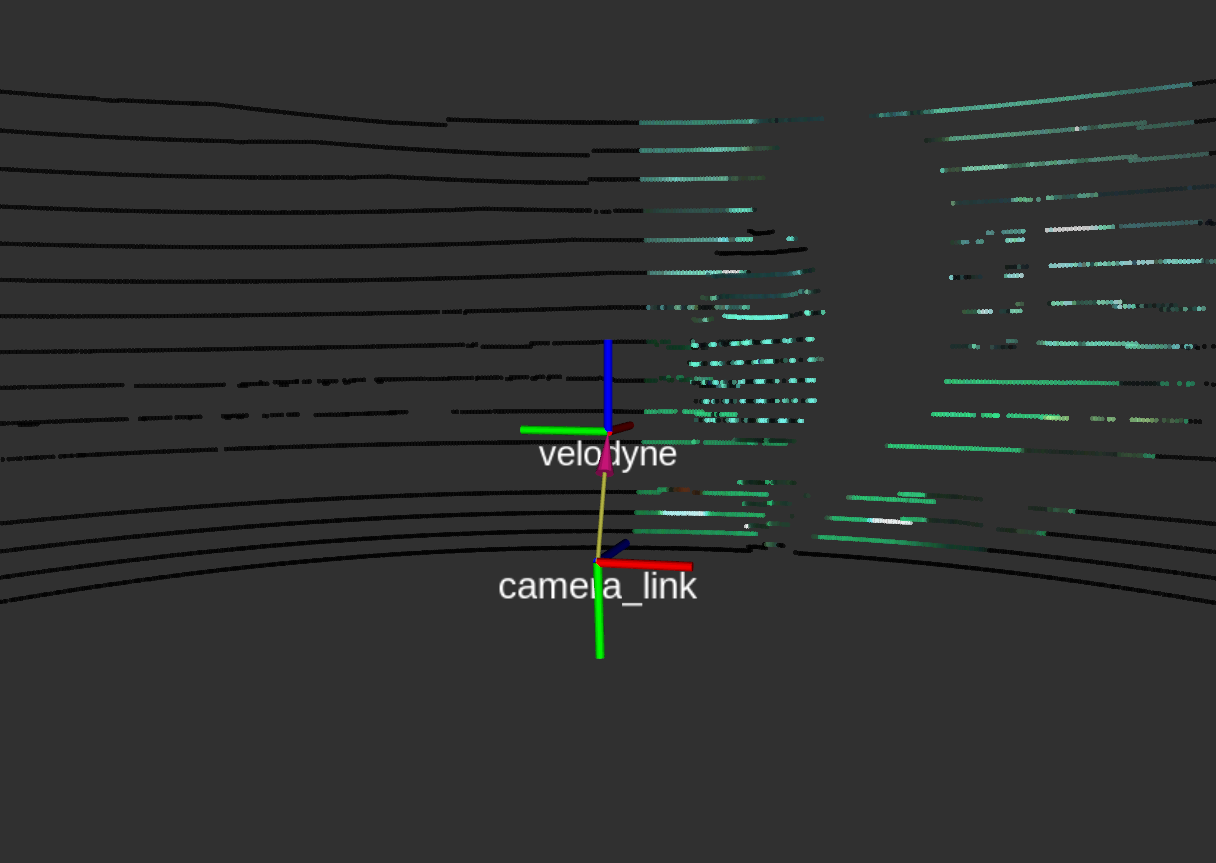
\includegraphics[width=\textwidth]{img/sensor_fusion/cambada_fusion_points.png}
		\caption{}
		\label{fig:sensor-fusion:cambada-points}
	\end{subfigure}
	\qquad
	\begin{subfigure}[t]{0.45\textwidth}
		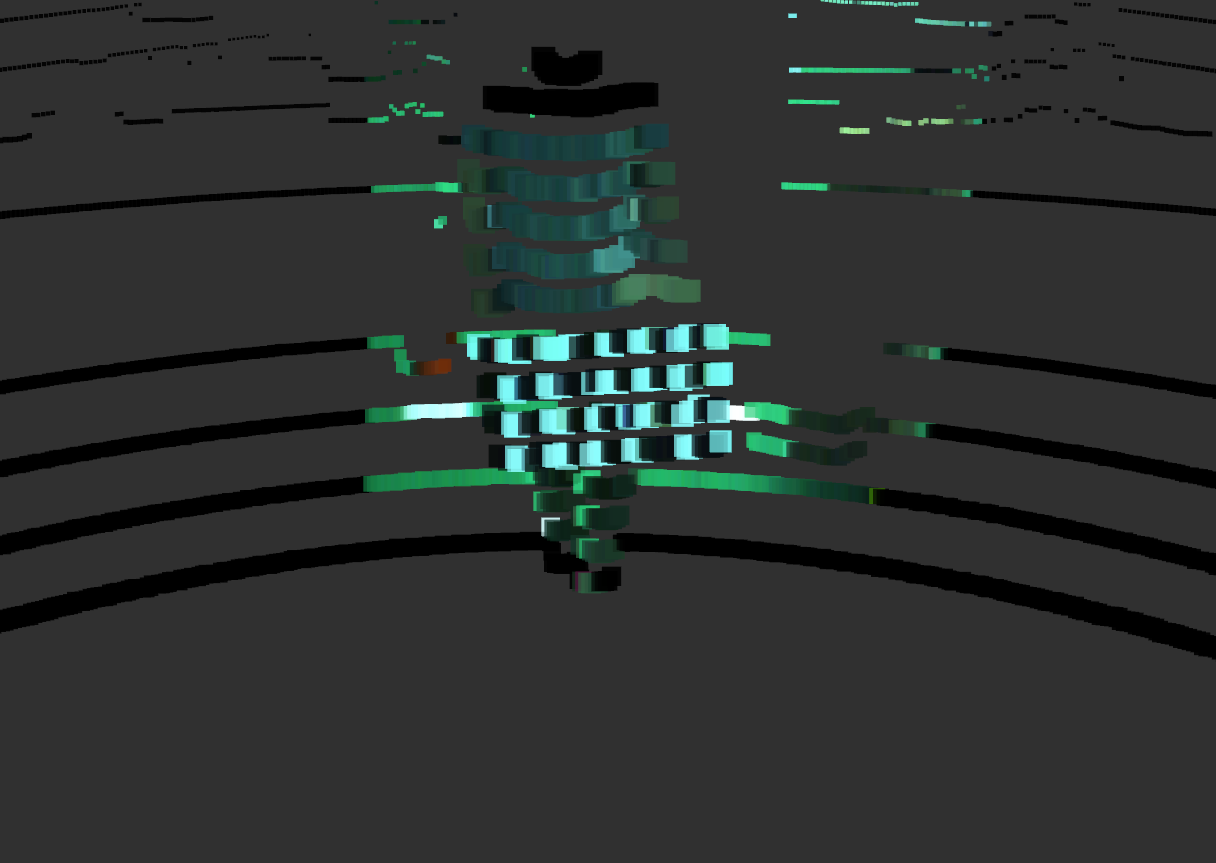
\includegraphics[width=\textwidth]{img/sensor_fusion/cambada_fusion_squares.png}
	\caption{}%The rectangles presented on the image have a size 4 cm and a transparency of 70\%.}
		\label{fig:sensor-fusion:cambada-squares}
	\end{subfigure}
	\caption[Colored point clouds computed for the datasets on \acs{irislab}.]{Data fusion between the camera and the \ac{lidar} on a \ac{msl} field. The colored point cloud is presented on sub-figure: (\subref{fig:sensor-fusion:cambada-points}) with points of 4 pixels and 70\% of transparency, with the coordinate frames also shown; (\subref{fig:sensor-fusion:cambada-squares}) with squares of \SI{4}{\centi\meter} of size and a transparency of 70\%.}
	\label{fig:cambada-sensor-fusion}
\end{figure}

However, such results are obtained with a low point density (VLP-16 only has 16 lines of data\footnote{Actually, our Velodyne VLP-16 has one of its lasers out of order, therefore we only have 15 lines of data.}) and a distance from the objects to the camera (a few meters). 

Another test, from the preliminary stages of the work, show the colored point cloud on \ac{it} 2 Dark Room, a smaller room where some tests were carried. On this case, the objects of interest are closer, so the colored point cloud has a better point cloud density, as shown in Figure~\ref{fig:dark-room-sensor-fusion}, 

\begin{figure}[!ht]
	\centering
	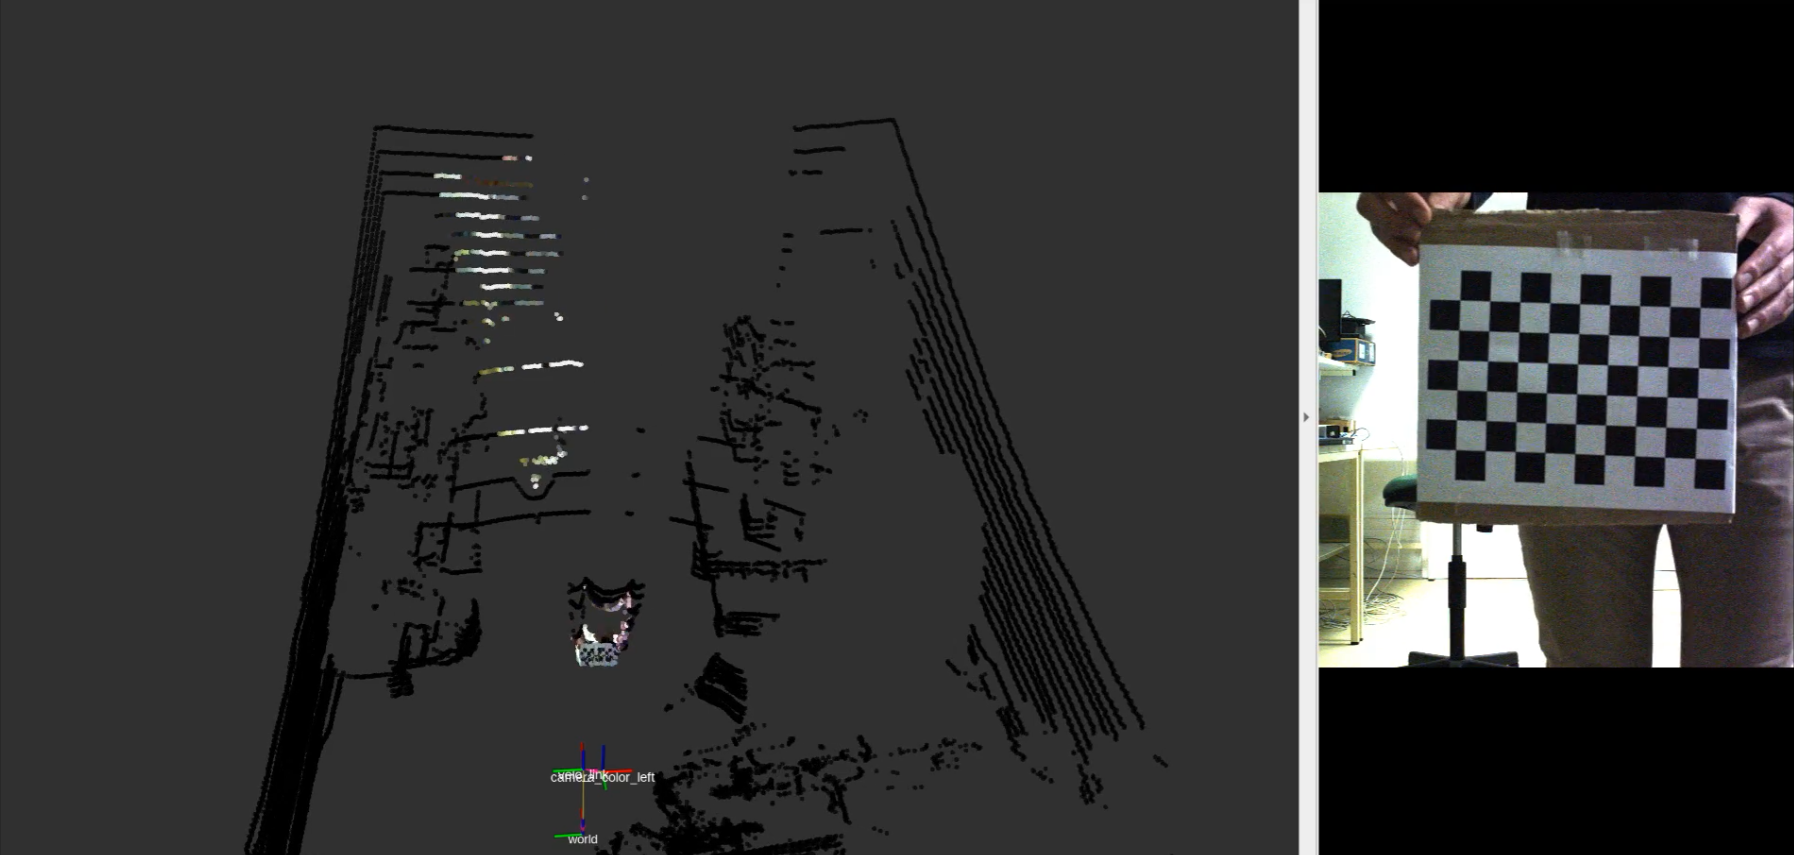
\includegraphics[width=0.7\textwidth]{img/sensor_fusion/dark-room-sensor-fusion.png}
\caption[Example of preliminar data fusion on \acs{it} 2 Dark Room.]{Data fusion between the \ac{lidar} and the camera data. On the left is the colored point cloud and on the right the image. The difference between this and the colored point clouds presented in Figure~\ref{fig:cambada-sensor-fusion} is that the objects of interest are closer to the camera and the experimental setup is placed inside a small room.}
	\label{fig:dark-room-sensor-fusion}
\end{figure}

\subsection{\acs{kitti} Dataset}
\label{subsec:sensor-fusion:kitti}
Applying the developed nodes to \ac{kitti} data set, which uses a Velodyne HDL-64E, with 64 pairs of laser beams and photodetectors, having 4 times more lines than our setup, results on the colored point cloud presented in Figure~\ref{fig:kitti-sensor-fusion}. This cloud has some differences when compared with the figures~\ref{fig:cambada-sensor-fusion} and~\ref{fig:dark-room-sensor-fusion}, such as:

\begin{itemize}
	\item The increase of photorealism in the colored point cloud, due to the increase in the number of laser beams;
	\item The dynamic scenario on \ac{kitti} dataset, compared to ours static experimental scenario.
\end{itemize}

In Figure~\ref{fig:kitti-sensor-fusion}, a mismatch between the top and bottom part of the sub-figures can be observed, even if accounting for the different \ac{fov} and view port for the camera and \ac{lidar}. This mismatch is due to the processing delay introduced by the point cloud coloring \ac{ros} node, which results on the colored point cloud being published to the \ac{ros} network with a large delay and our implementation cannot keep up with the publishing demand of \ac{kitti}'s dataset data rate, which causes the mismatch between the points positioning along the car direction of movement. Such mismatch and delay, however, is only due to the hardware  specifications running the algorithm, as is completely eliminated by using a computer with better specifications, specially on \ac{ram}, \ac{gpu} and \ac{cpu}.

\begin{figure}[!ht]
	\centering
	\begin{subfigure}[c]{0.8\textwidth}
		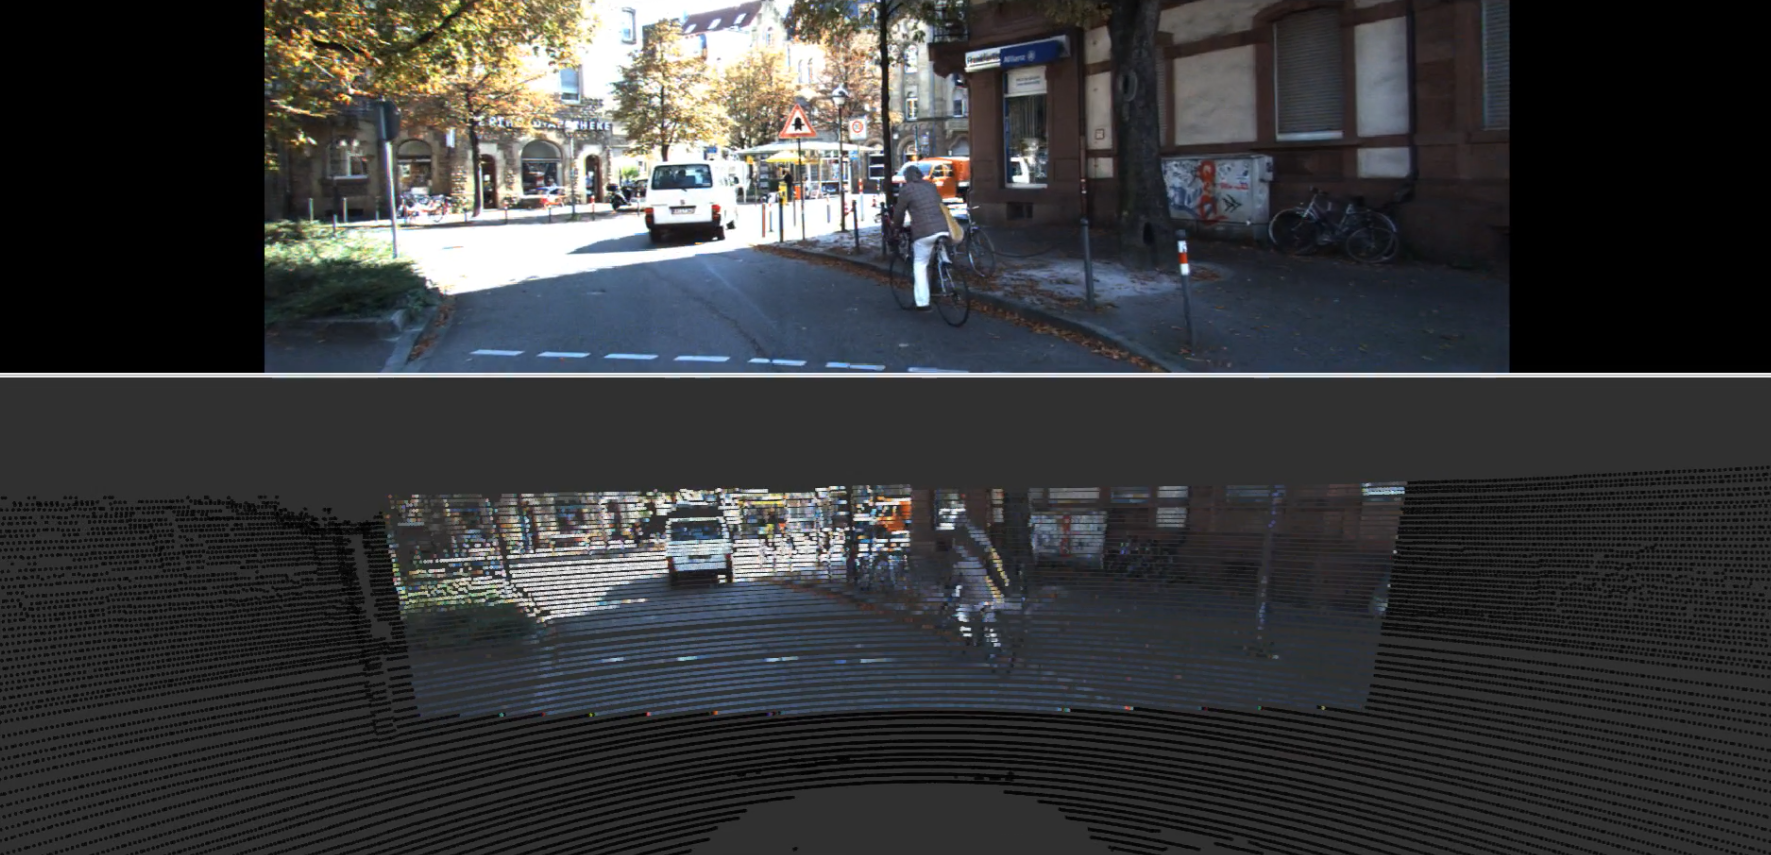
\includegraphics[width=\textwidth]{img/sensor_fusion/kitti-sensor-fusion-1.png}
		\caption{}
		\label{fig:kitti-sensor-fusion-1}
	\end{subfigure}
	\\ \vspace{4mm}
	\begin{subfigure}[c]{0.8\textwidth}
		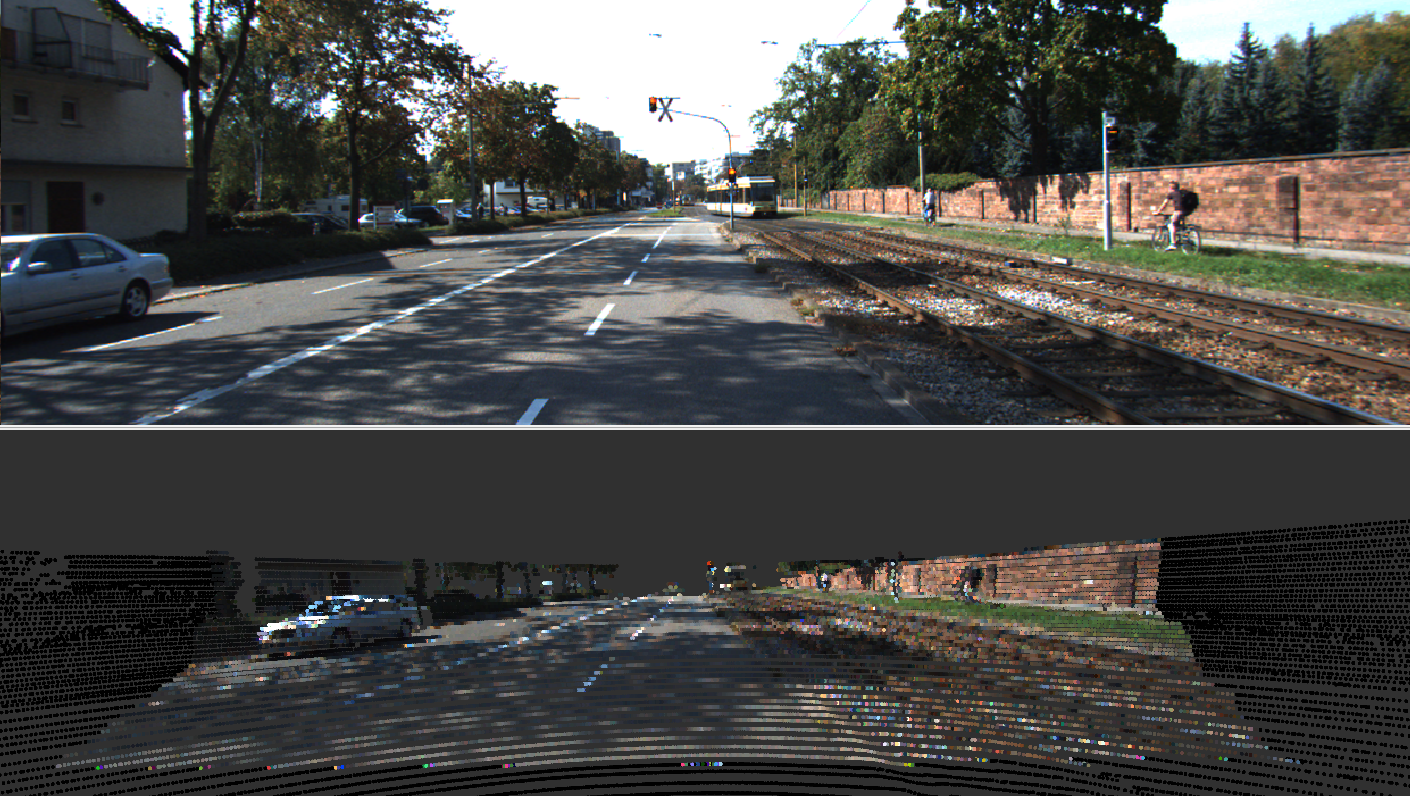
\includegraphics[width=\textwidth]{img/sensor_fusion/kitti-sensor-fusion-2.png}
		\caption{}
		\label{fig:kitti-sensor-fusion-2}
	\end{subfigure}
	\caption[Example of data fusion on \acs{kitti} dataset.]{Data fusion between camera and \ac{lidar} applied to the \ac{kitti} dataset. On the top there is the image and on the bottom the colored point cloud, displayed in points with 6 pixels of size and 50\% of transparency. Note that there is a mismatch between the image being shown and the image used to create the colored point cloud of 2 frames. In sub-Figure~(\subref{fig:kitti-sensor-fusion-1}), a cyclist and the car can clearly been identified on the colored point cloud and in sub-Figure~(\subref{fig:kitti-sensor-fusion-2}), the car, the wall, the road lines and the shadows can clearly be seen on the colored point cloud.}
	\label{fig:kitti-sensor-fusion}
\end{figure}


\subsection{Impact of Point Cloud Density}
In Figure~\ref{fig:dark-room-sensor-fusion}, it is evident that coloring a point cloud results on the loss of many high level features that are present on an image. On the resulting colored point cloud can be difficult to distinguish any objects with the original image and if the viewer does not know the scene being displayed.

Such loss of context and high level features is due to the scarce nature of a point cloud in relation to the camera. A 16-beam \ac{lidar} would only have 16 rows of depth data, while a 5\ac{mp} image will have 1920 rows of pixels. That relation means that only 0.83\% of the image rows will have correspondences on the point cloud. Such is the case of our experimental data.

If the number of pixels is considered instead, assuming a high camera \ac{fov} of \SI{90}{\degree} (which is not our case, since monocular camera \ac{fov} is normally lower), a quarter of the point cloud points, $\approx 7200$ points are candidates for correspondences between camera and \ac{lidar}, resulting in only 0.14\% of pixels on the image having a correspondence to the point cloud. 

For \ac{kitti}'s dataset, a 2\ac{mp} camera is used and a 64 beams \ac{lidar}, which yields almost 6\% of the image rows having correspondences and $\approx 5.76\%$ of the image pixels having a corresponding point on the \ac{lidar} point cloud. Comparing with our setup, \ac{kitti} has a number of correspondences between image pixels and point cloud points 41 times higher, which results on the clear difference in photorealism between figures~\ref{fig:cambada-sensor-fusion} and~\ref{fig:dark-room-sensor-fusion} with Figure~\ref{fig:kitti-sensor-fusion}.

Therefore, we can conclude that merging color with the point cloud depth information, on the way we implemented it, is not a feasible solution either to generate better data for autonomous vehicles, assessing the calibration results or possibly mitigating the interference, due to the losses in the information contained on the image. A solution to tackle such sparsity of the \ac{lidar} data and its impacts on point cloud coloring would be to generate a mesh cloud  from a point cloud and then performing mesh cloud coloring and/or interpolation of the point cloud, in order to increase it point cloud density. Obviously, using a \ac{lidar} with a higher number of laser beams will help mitigate this problem.

\section{Final Remarks}
In this chapter, image and point cloud data are fused to create a ``colored point cloud'': a tridimensional point representation of the scene with depth and color information. The perks of such process are detailed in this chapter and a brief discussion of data fusion representation possibilities is provided: color on point cloud points or depth points overlapped on a 2D image. Our implementation chooses the former and two possible implementation are discussed.  

To implement such a data fusion, the rigid body transformation between the \ac{lidar} and camera must be determined, following the procedures in Section~\ref{sec:calibration:extrinsic} and the camera and \ac{lidar} must be intrinsically calibrated as indicated in Sections~\ref{sec:calibration:camera} and~\ref{sec:calibration:lidar}. Our implementation, a single online \ac{ros} node, assumes these steps are undertaken and listens to the \ac{lidar} and camera data, synchronizing it and coloring the point cloud. To determine the color of the points, we use the $2D \rightarrow 3D$ correspondences.

The results from this chapter show, visually, that the extrinsic calibration developed in Chapter~\ref{chapter:calibration} is correctly done. However, when comparing the results obtained on \ac{kitti} dataset with ours, our implementation lacks point cloud density to generate a photorealistic colored point cloud. Such drawback is caused by the low resolution of our \ac{lidar}\footnote{It should be noted that higher resolution \acp{lidar} for automotive were not available.}, and it reveals that this approach is not the correct one to create good models for autonomous driving. We would have hopped that by using a camera we could help mitigate this problem by merging data together, but this crude approach of projecting data from one coordinate frame to another is clearly not enough. We also briefly discuss the possibility to interpolate the data, to create a better model.


From this chapter, the main outcome is the understanding of transforming and fusing data from one to another, along with some insights on the possibility to use data/sensor fusion to mitigate the \ac{lidar} interference. Also, one takeout are the algorithms and libraries for point cloud to image re-projection, which are used to estimate the point cloud bounding box from the image bounding boxes, in Chapter~\ref{chapter:object-detection} since the mathematical description of the two problems is similar.




% End of Thesis text ---------------------------------------------------------
% Including files is advised:


%Appendix

\backmatter


%Print all used references

\begingroup
\renewcommand{\bibfont}{\footnotesize}

%Redefine References name
\defbibheading{bibliography}[Referências]{
	\chapter{#1}
}
\SingleSpacing
\setlength\bibitemsep{8pt}
\printbibliography[heading=bibliography]
\endgroup


%Load appendix
%\section{Appendix A: RECPAD paper} 
\label{appendix:recpad} 
\acl{recpad} paper.
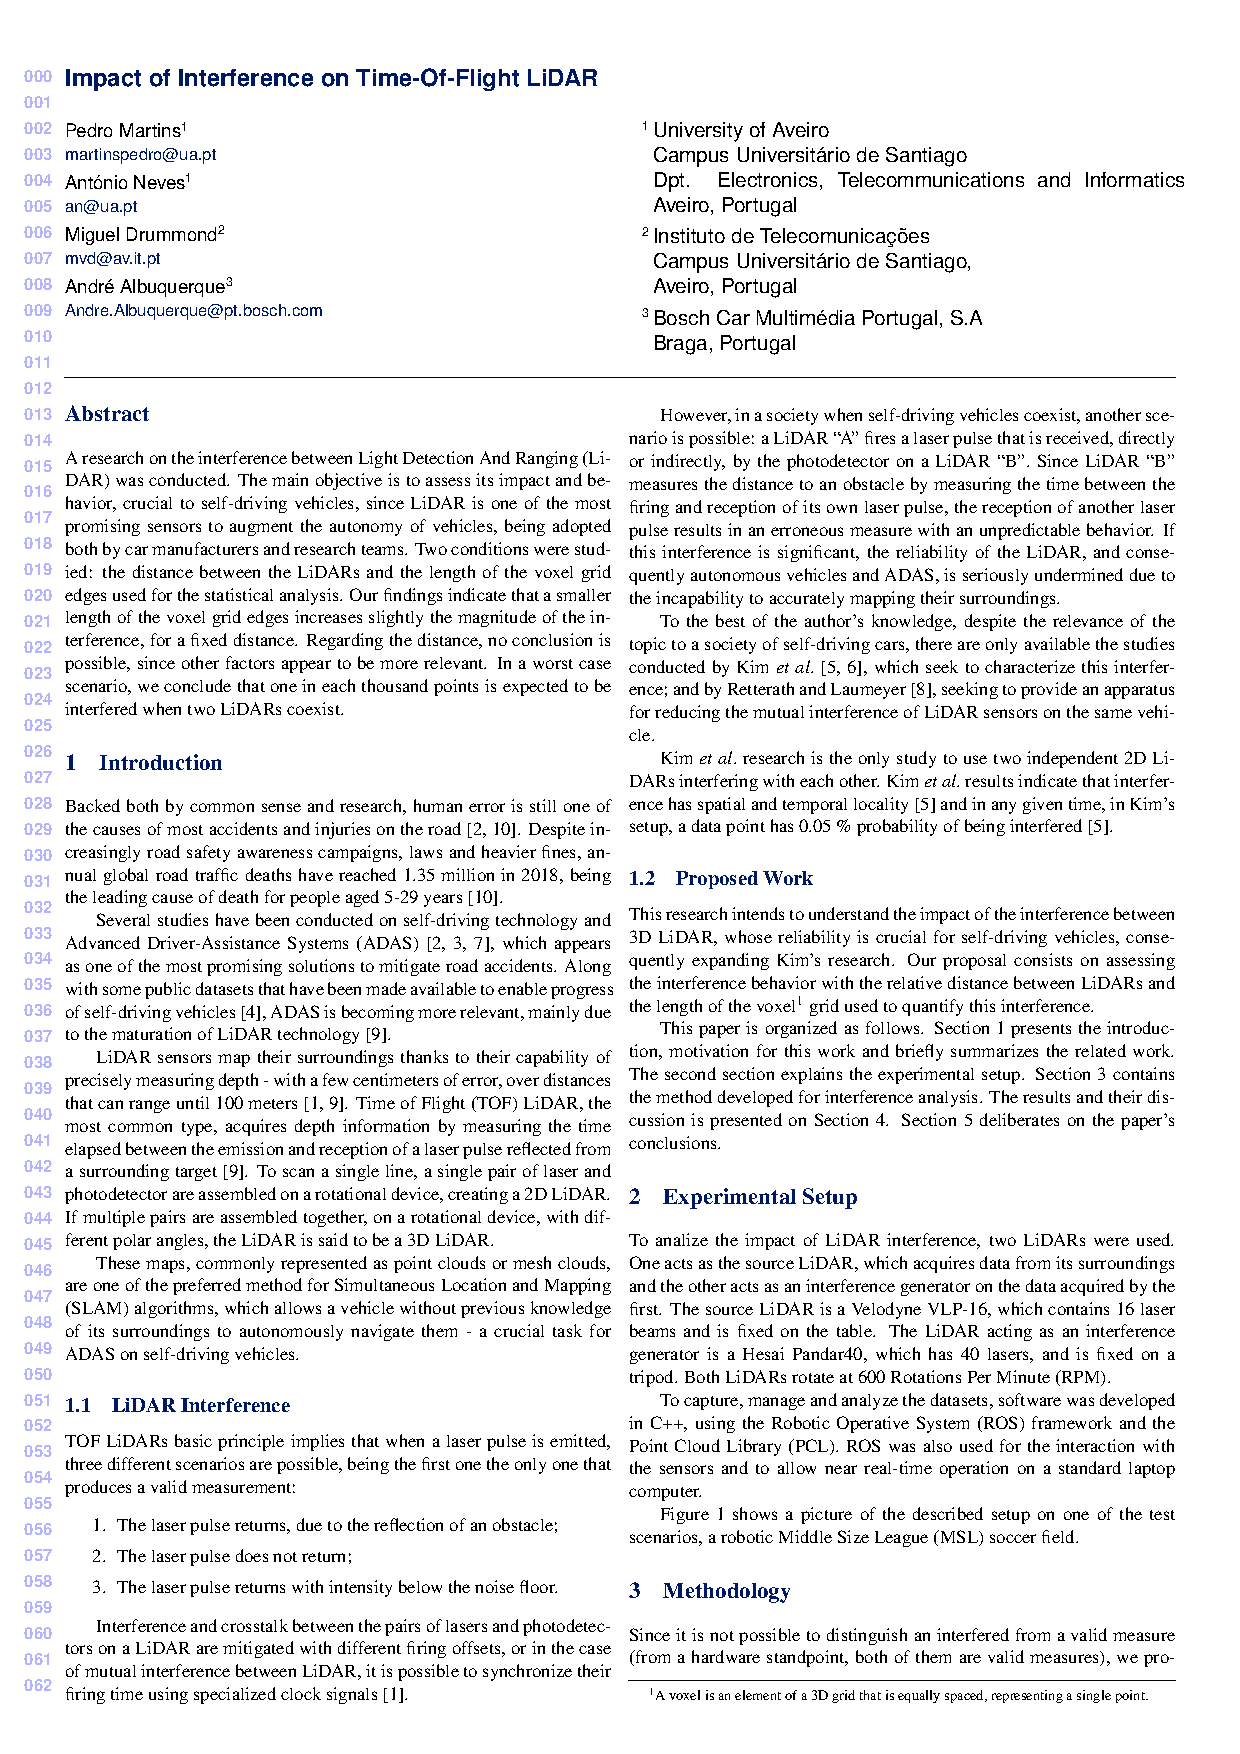
\includepdf[pages=-]{appendix/RECPAD2019.pdf}




\end{document}
